\documentclass[a4paper, 12pt, oneside]{article}
\usepackage[hidelinks]{hyperref}
\usepackage{graphicx}
% \usepackage[utf8]{inputenc}
% \usepackage{polski}
\usepackage{listings}
\usepackage[backend=biber, style=numeric-comp, alldates=iso, seconds=true, sorting=none]{biblatex}
\addbibresource{9-references.bib}
%\bibliographystyle{unsrt}
\usepackage{xcolor}
\usepackage{csquotes}
\usepackage{multirow}
%\usepackage{indentfirst}
\usepackage{url}
\usepackage{float}
\usepackage[a4paper]{geometry}
\usepackage[nogroupskip, acronym, toc]{glossaries}
\usepackage[automake]{glossaries-extra}

% Graph plotting
\usepackage{siunitx}
\usepackage{tikz} % To generate the plot from csv
\usepackage{pgfplots}
\usepgfplotslibrary{groupplots}

\pgfplotsset{compat=newest} % Allows to place the legend below plot
\usepgfplotslibrary{units} % Allows to enter the units nicely
\usepackage[skip=10pt]{caption}

\sisetup{
  round-mode          = places,
  round-precision     = 2,
}

\definecolor{codegreen}{rgb}{0,0.6,0}
\definecolor{codegray}{rgb}{0.5,0.5,0.5}
\definecolor{codepurple}{rgb}{0.58,0,0.82}
\definecolor{backcolour}{rgb}{0.95,0.95,0.92}

\lstdefinestyle{mystyle}{
  backgroundcolor=\color{backcolour},   
    commentstyle=\color{codegreen},
    keywordstyle=\color{magenta},
    numberstyle=\tiny\color{codegray},
    stringstyle=\color{codepurple},
    basicstyle=\ttfamily\footnotesize,
    breakatwhitespace=false,         
    breaklines=true,                 
    captionpos=b,                    
    keepspaces=true,                 
    numbers=left,                    
    numbersep=5pt,                  
    showspaces=false,                
    showstringspaces=false,
    showtabs=false,                  
    tabsize=2
}

\lstset{style=mystyle}

\setabbreviationstyle{long-short}

\makeglossaries

% Economics

\newabbreviation{forex}{FOREX}{foreign exchange}
\newabbreviation{otc}{OTC}{over-the-counter}
\newabbreviation{emh}{EMH}{efficient market hypothesis}
\newabbreviation{ecb}{ECB}{european central bank}
\newabbreviation{eer}{EER}{effective exchange rates}
\newabbreviation{cpi}{CPI}{consumer price index}

% Models

\newabbreviation{ai}{AI}{artificial intelligence}
\newabbreviation{nn}{NN}{neural network}
\newabbreviation{ann}{ANN}{artificial \glsxtrshort{nn}}
\newabbreviation{svm}{SVM}{support vector machine}
\newabbreviation{svr}{SVR}{support vector regression}
\newabbreviation{rf}{RF}{random forest}
\newabbreviation{rnn}{RNN}{recurrent \glsxtrshort{nn}}
\newabbreviation{cnn}{CNN}{convolutional \glsxtrshort{nn}}
\newabbreviation{lstm}{LSTM}{long short-term memory}
\newabbreviation{mlp}{MLP}{multi layer perceptron}
\newabbreviation{sbp}{SBP}{standard backpropagation}
\newabbreviation{scg}{SCG}{scaled conjugate gradient}
\newabbreviation{bpr}{BPR}{backpropagation with baysian regularization}
\newabbreviation{slp}{SLP}{single layer perceptron}
\newabbreviation{dt}{DT}{decision tree}
\newabbreviation{rcgpann}{RCGPANN}{recurrent cartesian genetic programming evolved \glsxtrshort{ann}}
\newabbreviation{gmminf}{GMMINF}{gaussian mixture model initialized neuro-fuzzy}
\newabbreviation{anova}{ANOVA}{analysis of variance}
\newabbreviation{rar}{RAR}{robust linear autoregression}

% Algorithms

\newabbreviation{tpe}{TPE}{Tree-structured Parzen Estimator}

% Evaluation

\newabbreviation{cv}{CV}{cross validation}

% Feature selection

\newabbreviation{rfecv}{RFECV}{recursive feature elimination with \glsxtrshort{cv}}

% Time series prediction models

\newabbreviation{ar}{AR}{autoregressive}
\newabbreviation{ma}{MA}{moving-average}
\newabbreviation{arma}{ARMA}{autoregressive moving-average}
\newabbreviation{es}{ES}{exponential smoothing}
\newabbreviation{arima}{ARIMA}{autoregressive integrated moving average}
\newabbreviation{rw}{RW}{random walk}
\newabbreviation{arch}{ARCH}{auto-regressive conditional heteroskedasticity}
\newabbreviation{garch}{GARCH}{general auto-regressive conditional heteroskedasticity}
\newabbreviation{var}{VAR}{vector autoregressive}
\newabbreviation{vec}{VEC}{vector error correction}

% Activation functions

\newabbreviation{relu}{relu}{rectified linear unit}
\newabbreviation{tanh}{tanh}{hyperbolic tangent}

% SVM kernel

\newabbreviation{rbf}{RBF}{radial basis function}
\newabbreviation{sgds}{SGD}{stochastic gradient descent}
\newabbreviation{lbfgs}{LBFGS}{Limited memory Broyden–Fletcher–Goldfarb–Shanno algorithm}

% Currencies

\newabbreviation{uah}{UAH}{Ukraine hryvnia}
\newabbreviation{twd}{TWD}{New Taiwan dollar}
\newabbreviation{sar}{SAR}{Saudi riyal}
\newabbreviation{pen}{PEN}{Peru nuevo sol}
\newabbreviation{mad}{MAD}{Moroccan dirham}
\newabbreviation{dzd}{DZD}{Algerian dinar}
\newabbreviation{cop}{COP}{Colombian peso}
\newabbreviation{clp}{CLP}{Chilean peso}
\newabbreviation{ars}{ARS}{Argentine peso}
\newabbreviation{aed}{AED}{United Arab Emirates dirham}
\newabbreviation{usd}{USD}{United States Dollar}
\newabbreviation{jpy}{JPY}{Japanese Yen}
\newabbreviation{bgn}{BGN}{Bulgarian Lev}
\newabbreviation{cyp}{CYP}{Cypriot Pound}
\newabbreviation{czk}{CZK}{Czech Koruna}
\newabbreviation{dkk}{DKK}{Danish Krone}
\newabbreviation{eek}{EEK}{Estonian Kroon}
\newabbreviation{gbp}{GBP}{British Pound}
\newabbreviation{huf}{HUF}{Hungarian Forint}
\newabbreviation{ltl}{LTL}{Lithuanian Litas}
\newabbreviation{lvl}{LVL}{Latvian Lats}
\newabbreviation{mtl}{MTL}{Maltese Lira}
\newabbreviation{pln}{PLN}{Polish Zloty}
\newabbreviation{rol}{ROL}{Romanian Leu}
\newabbreviation{ron}{RON}{Romanian Leu}
\newabbreviation{sek}{SEK}{Swedish Krona}
\newabbreviation{sit}{SIT}{Slovenian Tolar}
\newabbreviation{skk}{SKK}{Slovak Koruna}
\newabbreviation{chf}{CHF}{Swiss Franc}
\newabbreviation{isk}{ISK}{Icelandic Krona}
\newabbreviation{nok}{NOK}{Norwegian Krone}
\newabbreviation{hrk}{HRK}{Croatian Kuna}
\newabbreviation{rub}{RUB}{Russian Ruble}
\newabbreviation{trl}{TRL}{Turkish Lira}
\newabbreviation{try}{TRY}{Turkish Lira}
\newabbreviation{aud}{AUD}{Australian Dollar}
\newabbreviation{brl}{BRL}{Brazilian Real}
\newabbreviation{cad}{CAD}{Canadian Dollar}
\newabbreviation{cny}{CNY}{Chinese Yuan}
\newabbreviation{hkd}{HKD}{Hong Kong Dollar}
\newabbreviation{idr}{IDR}{Indonesian Rupiah}
\newabbreviation{ils}{ILS}{Israeli Shekel}
\newabbreviation{inr}{INR}{Indian Rupee}
\newabbreviation{krw}{KRW}{South Korean Won}
\newabbreviation{mxn}{MXN}{Mexican Peso}
\newabbreviation{myr}{MYR}{Malaysian Ringgit}
\newabbreviation{nzd}{NZD}{New Zealand Dollar}
\newabbreviation{php}{PHP}{Philippine Peso}
\newabbreviation{sgd}{SGD}{Singapore Dollar}
\newabbreviation{thb}{THB}{Thai Baht}
\newabbreviation{zar}{ZAR}{South African Rand}

% Other currencies

\newabbreviation{eur}{EUR}{Euro}
\newabbreviation{pkr}{PKR}{Pakistani Rupee}

% Measures

\newabbreviation{mse}{MSE}{mean square error}
\newabbreviation{mae}{MAE}{mean absolute error}
\newabbreviation{mape}{MAPE}{mean absolute percentage error}
\newabbreviation{ds}{DS}{directional symmetry}
\newabbreviation{oob}{OOB}{out-of-bag}



\begin{document}

\include{0-title-page}

\newgeometry{margin=3cm}
\maketitle

% \section*{Abstract}\label{Abstract}

The purpose of this master's thesis is to explore the applicability of \glsxtrlong{ai} algorithms for predicting exchange rates. Forecasting exchange rates is a significant challenge for both financial institutions and individual investors. The thesis focuses on analysing various machine learning algorithms, such as \glsxtrlongpl{nn}, \glsxtrlongpl{svm}, and \glsxtrlongpl{rf}, for their effectiveness and accuracy in forecasting currency values.\\

The research methodology is based on the analysis of historical currency data and its processing using selected artificial intelligence algorithms. The research to be carried out will include cleaning and preparation of data, selection of appropriate features, and optimization of model parameters. This will be followed by a comparison of the results obtained using different techniques, in order to determine the most effective methods in the context of exchange rate predictions.\\

The expected result of the work is the development of an exchange rate prediction model with high accuracy, which could be applied in practice to support investment decisions and risk management.


% \newgeometry{tmargin=1.7cm}
{\small\tableofcontents}
% \restoregeometry

\newgeometry{margin=3cm}
\section{Introduction}\label{Introduction}

\subsection{Exchange rates}\label{Exchange rates}

Since the fall of the Bretton Woods system of fixed exchange rates in 1976 and the establishment of floating exchange rates with the Jamaica Accords, the need for accurate forecasting of exchange rates has become increasingly important. The primary reason for this is the need for effective risk management, especially for businesses, investors, currency traders, governments, and banks. Knowing whether the value of a currency will rise or fall ahead of time allows not only for the mitigation of adverse currency movements, but also for well-timed and potentially highly profitable investment decisions.

Unfortunately, exchange rates are notoriously difficult to predict as they exhibit a complex non-linear nature that is dependant on a wide range of variables including macroeconomic and microeconomic factors.

Given the challenges in forecasting exchange rates using traditional econometric models, researchers have increasingly turned to the application of artificial intelligence (AI) algorithms as a potential solution. AI-based approaches, such as neural networks, genetic algorithms, and machine learning techniques, have shown promise in their ability to capture the complex, nonlinear relationships inherent in exchange rate dynamics. These methods have the potential to outperform traditional forecasting models by identifying patterns and relationships that may be difficult for human analysts to discern.

\subsection{Literature review}\label{Literature review}



\section{Theoretical foundations}\label{Theoretical foundations}

The following is an overview of the most important topics of significance to this research paper.

\subsection{Time series models}\label{Time series models}

In the domain of time series forecasting many models have been developed. These models can be subdivided into univariate and multivariate models. Univariate track a single variable and make predictions based on the historical values of that same variable. Multivariate track the mutual dependance of multiple variables and make predictions on there future values.

\subsubsection{Univariate}\label{Univariate}

The most important univariate models that have been developed over the years include:

\begin{itemize}
    \item \Gls{ar} \cite{whittle} - expresses the current value as a linear combination of $p$ historical values. \Glsxtrshort{ar}$(p)$ denotes an \glsxtrlong{ar} model of order $p$. The model is mathematically defined as follows:

        $X_{t} =  \varepsilon_{t} + \sum_{i=1}^{p}\phi_{i}X_{t-i}$

        where:
        \begin{itemize}
            \item $X_{t}, X_{t-i}$ are the values of the time series at time $t$ and $t-i$.
            \item $\phi_{i}$ are the coefficient for values at different time offsets.
            \item $\varepsilon_{t}$ is the random variable representing white noise.
        \end{itemize}
    \item \Gls{ma} \cite{whittle} - expresses the current value as a linear combination of $p$ historical error terms. \Glsxtrshort{ma}$(q)$ denotes an \glsxtrlong{ma} model of order $q$. The model is mathematically defined as follows:
        
        $X_{t} = \mu + \varepsilon_{t} + \sum_{i=1}^{q}\theta_{i}\varepsilon_{t-i}$
        
        where:
        \begin{itemize}
            \item $\mu$ is the the mean of the series.
            \item $X_{t}, X_{t-i}$ are the values of the time series at time $t$ and $t-i$.
            \item $\theta_{i}$ are the coefficient for error terms at different time offsets.
            \item $\varepsilon_{t-i}$ are the the white noise error terms at time $t-i$.
        \end{itemize}

    \item \Gls{arma} \cite{whittle} - combines the \gls{ar} and \gls{ma} models. \Glsxtrshort{arma}$(p)$ denotes an model with $p$ autoregressive terms and $q$ moving-average terms. \gls{arma} requires the time series to be stationary. The model is mathematically defined as follows:

        $X_{t} =  \varepsilon_{t} + \sum_{i=1}^{p}\phi_{i}X_{t-i} + \sum_{i=1}^{q}\theta_{i}\varepsilon_{t-i}$

    \item \Gls{es} \cite{brown,holt} - expresses the current value in a time series as a exponentially weighted combination of its past values where the most recent values have the most significance. Its mathematical representation is a follows:

        $S_{t} = \alpha X_{t} + (1 - \alpha)S_{t-1}$

        where:
        \begin{itemize}
            \item $S_{t}, S_{t-1}$ are the values of the smoothed time series at time $t$ and $t-1$.
            \item $\alpha$ is the smoothing factor.
            \item $X_{t}$ is the value of the time series at time $t$.
        \end{itemize}

    \item \Gls{arima} \cite{box-jenkins} - is a generalization of the \gls{arma} model which requires non-stationary series to be differenced in order for them to achieve stationarity. \gls{arima} models are denoted by: \gls{arima}$(p, d, q)$ where $p$ is the order of the \gls{ar} model, $d$ is the degree of differencing and $q$ is the order of the \gls{ma} model. Using the Box-Jenkins method allows for the selection of optimal parameters for an \gls{arima} model enabling the best fit of the model for the given time series.
    \item \Gls{rw} \cite{meese-rogoff} - is a naive model that proposes that changes between values in a time series are random and unrelated. There are two subvariants:
        \begin{itemize}
            \item \gls{rw} without drift defined as:

                $X_t = X_{t-1} + \varepsilon_t$

            \item \gls{rw} with drift defined as:
        
                $X_t = X_{t-1} + a + \varepsilon_t$

        \end{itemize}

    where:

    \begin{itemize}
            \item $X_{t}, X_{t-1}$ is the value of the time series at time $t$ and $t - 1$.
            \item $\varepsilon_t$ is the random step at time $t$.
            \item $a$ - is a constant that determines the trend of the series.
    \end{itemize}

        The \gls{rw} without drift is often used as a benchmark for various forecasting models.

    \item \Gls{arch} \cite{engle} - is a model that describes the conditional variance of a time series as an \gls{ar} combination of past squared errors. \Glsxtrshort{arch}$(p)$ denotes an \glsxtrlong{arch} model of order $p$. The time series is described by the following equation:

        $\sigma_{t}^2 = \alpha_{0} + \sum_{i=1}^{p}\alpha_{i}\varepsilon_{t-i}^2$

    where:
    \begin{itemize}
        \item $\sigma_{t}^2$ is the conditional variance.
        \item $\alpha_{0}$ is a constant term that sets the baseline level of variance.
        \item $\alpha_{i}$ are the coefficients that determine the weight of previous error terms.
        \item $\varepsilon_{t-i}$ are values of previous error terms.
    \end{itemize}

    \item \Gls{garch} \cite{bollerslev} - is an extension of \gls{arch} that allows the conditional variance to be an \gls{arma} process, rather than just an \gls{ar} process as in \gls{arch}. The \Glsxtrshort{garch}(p,q) model is described by the equation:

        $\sigma_{t}^2 = \alpha_{0} + \sum_{i=1}^{p}\alpha_{i}\varepsilon_{t-i}^2 + \sum_{j=1}^{q}\beta_{j}\sigma_{t-j}^2$

        where:
    \begin{itemize}
        \item $\sigma_{t}^2$ is the conditional variance.
        \item $\alpha_{0}$ is a constant term that sets the baseline level of variance.
        \item $p$ is the order of the \gls{ar} term.
        \item $q$ is the order of the \gls{ma} term.
        \item $\alpha_{i}$ are the coefficients of the \gls{ar} terms.
        \item $\beta_{j}$  are the coefficients of the \gls{ma} terms.
        \item $\varepsilon_{t-i}$ are values of previous error terms.
        \item $\sigma_{t-j}$ are the lagged conditional variance terms
    \end{itemize}

\end{itemize}

\subsubsection{Multivariate}\label{Multivariate}

Some of the most important multivariate models include:

\begin{itemize}
    \item \Gls{var} \cite{sims} - are a system of regressions where each variable is modeled as a function of its own lags and the lags of the other variables in the system. A $p$ order \gls{var} is denoted as \gls{var}$(p)$ \cite{deep-learning}. The model can be described as follows:

    $y_{t} = A_{1}y_{t-1} + A_{2}y_{t-2} + ... + A_{p}y_{t-p} + \mu_{t}$

    where:
        \begin{itemize}
            \item $y_{t}, y_{t-1}, y_{t-2}, y_{t-p}$ is a selection of endogenous variables.
            \item $A_{i}$ is an (N x N) matrix of autoregression coefficients.
            \item $\mu_{t}$ is an (N x 1) vector generalization of white noise.
        \end{itemize}

    \item \Gls{vec} \cite{johansen} - are a restricted form of VAR models used for non-stationary time series that are cointegrated. VEC models incorporate both the short-run dynamics and the long-run equilibrium relationships between the variables. \gls{vec} can have the following form:

        $\Delta x_{t} =\Pi x_{t-1} + \sum_{l=1}^{p-1}\Gamma_l\Delta x_{t-1} + Cd_{t} + \epsilon_{t}$

        where:
        \begin{itemize}
            \item $\Delta x$ is the first difference of the variables in vector $x$.
            \item $\Pi$ is a coefficient matrix of cointegrating relationships.
            \item $\Gamma$ is a coefficient matrix of the lags of differenced variables of $x$.
            \item $d$ is a vector of deterministic terms.
            \item $C$ coefficient matrix corresponding to $d$.
            \item $p$ is the lag order of the model in its \gls{var} form
            \item $\epsilon$ is an error term with zero mean and variance-covariance matrix $\sigma$.
        \end{itemize}
\end{itemize}

% \subsection{Econometric models}\label{Econometric models}
% 
% There are many models which attempt to specify a statistical relationship between various economic properties. The following are some of the most well known:
% 
% \cite{comparing,linear-vs-nn}
% 
% \subsubsection{Purchasing Power Parity (PPP)}\label{Purchasing Power Parity (PPP)}
% 
% \subsubsection{Uncovered Interest Rate Parity (UIP)}\label{Uncovered Interest Rate Parity (UIP)}
% 
% \subsubsection{Sticky Price Monetary (SP)}\label{Sticky Price Monetary (SP)}

\subsection{Artificial intelligence}\label{Artificial intelligence}

\glsxtrshort{ai}-based approaches, have shown promise in their ability to capture the complex, nonlinear relationships inherent in exchange rate dynamics. These methods have the potential to outperform traditional forecasting models by identifying patterns and relationships that may be difficult for human analysts to discern.

\subsubsection{Artificial neural network}\label{Artificial neural network}

\glsxtrshortpl{ann} are systems composed of interconnected nodes imitating in behaviour and structure a biological system of neurons. They take in a set of input signals and according to a set of rules produce a set of outputs \cite{linear-vs-nn}. Unlike other \glsxtrshort{ai} methods they do not make any assumptions about their input data \cite{ann-1}. \glsxtrshortpl{ann} are categorized as non-parametric (nonlinear) statistical methods and are used as universal function approximators for any continuous function \cite{svm-2}. There are many types of \glsxtrlong{ann} including: \glspl{rnn}, \glspl{cnn}, \gls{lstm} and feedforward networks among others. One of the most commonly used types of \glspl{nn} is the \gls{mlp} which is a type of feedforward \glsxtrshort{ann}.

An \glsxtrshort{mlp} consists of multiple layers made up of nodes (neurons). At its simplest we have a \gls{slp} a \glsxtrshort{nn} which consists of only two layers an input layer and an output layer. In more complex cases where non linear functions need to be modeled one or more intermediary hidden layers are added \cite{lstm-mlp-rf,svm-2}. A diagram of a simple three layer \gls{ann} is presented in figure \ref{fig:nn}. The neurons of one layer are linked to the neurons of the following layer. Each connection between neurons is assigned a weight. Additionally bias neurons with a positive value of one can be attached to the neurons of the hidden and output layers. The weighted sum of inputs to a neuron is calculated via a propagation function. The calculated value is then fed to the activation function of the neuron which introduces a degree of non-linearity simulating an activation threshold. The most commonly used are: \gls{relu}, sigmoid, \gls{tanh} and linear activation functions \cite{svm-2}.

\begin{figure}
    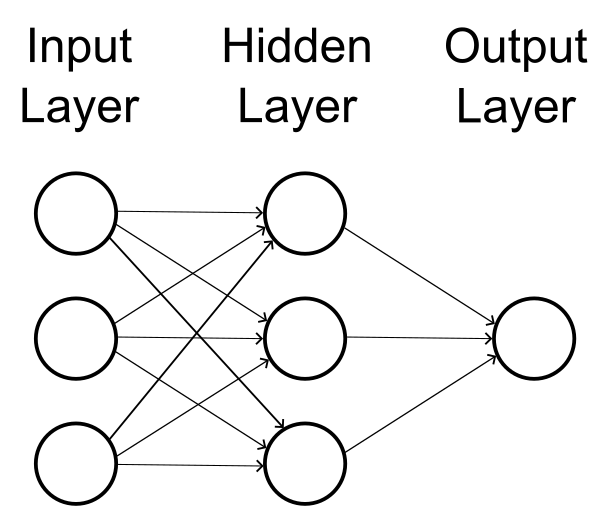
\includegraphics[width=0.5\textwidth]{images/neural-network.png}
    \centering
    \caption{A diagram portraying the structure of a simple three layer \gls{mlp}.}
    \label{fig:nn}
\end{figure}

The training of an \gls{ann} consists of the initial assignment of random weights to each of the neurons connections followed by an iterative minimization of the sum of squared errors over all of the training data. This process is carried out via a learning algorithm. The most commonly used are:
\begin{itemize}
    \item \Gls{sbp} which is a steepest gradient descent algorithm. For \gls{sbp} the weight $\omega_{j}$ in iteration $n$ is updated via the following equation:

$\Delta\omega_{j}(n) = -\eta\frac{\partial E}{\partial \omega_{j}}+\alpha\Delta\omega_{j}(n-1)$

    where:
        \begin{itemize}
            \item $\omega_{j}$ are the connection weights.
            \item $eta$ is the learning rate.
            \item $E$ is the sum of squared error.
            \item $alpha$ is the momentum factor.
            \item $n$ is the iteration.
        \end{itemize}

    \item \Gls{scg} is a method that searches along conjugate directions in successive iterations for faster convergence. Selection of search direction is governed by the following equations:

        $\omega_{k+1} = \omega_{k} + \alpha_{k}p_{k}$ \\
        $p_{k} = -E'(\omega) + \alpha_{k}p_{k+1}$

        where:
        \begin{itemize}
            \item $\omega_{k+1}, \omega_{k}$ are the connection weights.
            \item $\alpha$ is the momentum factor.
            \item $p_{k}, p_{k+1}$ are the conjugate directions in successive iterations.
            \item $E$ is the sum of squared error.
        \end{itemize}

    \item \Gls{bpr} is an extension of the \gls{sbp} algorithm which constrains network parameters via regularization. A modification is made to the loss function:

        $F = \gamma E + \frac{1 - \gamma}{n} \sum_{j=1}^{n}\omega_{j}^2$

        where:
        \begin{itemize}
            \item $F$ is the loss function.
            \item $\gamma$ is the performance ratio parameter.
            \item $E$ is the sum squared error.
            \item $\omega_{j}$ are the connection weights.
            \item $n$ is the iteration.
        \end{itemize}
\end{itemize}

\subsubsection{Support vector machine}\label{Support vector machine}

The \glsxtrlong{svm} is a model designed for the supervised classification of labeled data belonging to two classes \cite{vapnik-svm}. It enables the discovery of an optimal line or hyperplane that maximizes the distance between each class in an N-dimensional space. An example of its application for a 2-dimensional space can be seen in figure \ref{fig:svm}. \gls{svm} can handle the linear separation of data as well as the non-linear separation of data via a kernel trick \cite{non-linear-svm}. The most popular non-linear kernels are the: polynomial kernel, \gls{rbf} and sigmoid kernel \cite{ibm-svm}. An extension of the original hard-margin \gls{svm} is the soft-margin \gls{svm}. The difference between them is that with the hard-margin \gls{svm} data points will be perfectly separated outside of the support vectors while soft-margin classification will allow some misclassification through the use of a slack variable \cite{vapnik-svm}.
The hard-margin \gls{svm} is defined as:\\

    $\underset{w, b}{minimize}\quad \frac{1}{2}\left\| \omega \right\|^2$

    $subject\ to\quad y_{i}(\omega^Tx_{i}-b) \ge 1\quad \forall i \in \{1,...,n\}$ \\

    where:
    \begin{itemize}
        \item $\omega$ is the normal vector to the hyperplane.
        \item $b$ is the distance of the hyperplane from the origin.
        \item $y_{i}$ is the class label for each training instance.
        \item $x_{i}$ is the feature vector for each training instance.
        \item $n$ is the total number of training instances.
    \end{itemize}

While the soft-margin \gls{svm} is defined as:\\

    $\underset{w, b, \zeta}{minimize}\quad \left\| w \right\|^2 + C\sum_{i=1}^{n}\zeta_{i}$

    $subject\ to\quad y_{i}(w^Tx_{i}-b) \ge 1 - \zeta_{i}$ \\

    where:
    \begin{itemize}
        \item $\omega$ is the normal vector to the hyperplane.
        \item $b$ is the distance of the hyperplane from the origin.
        \item $y_{i}$ is the class label for each training instance.
        \item $x_{i}$ is the feature vector for each training instance.
        \item $n$ is the total number of training instances.
        \item $C$ is the regularization parameter.
        \item $\zeta_{i}$ are the slack variables.
    \end{itemize}

Another extension of the \glsxtrshort{svm} is \gls{svr} which enables the application of \glsxtrshort{svm} to regression problems \cite{vapnik-svr,svr}.

\gls{svr} is defined as:\\

    $minimize\quad \frac{1}{2} \left\| w \right\|^2$

    $subject\ to\quad \left| y_{i} - \langle w,x_{i} \rangle - b \right| \le \varepsilon$\\

    where:
    \begin{itemize}
        \item $\omega$ is the normal vector to the hyperplane.
        \item $b$ is the distance of the hyperplane from the origin.
        \item $y_{i}$ is the class label for each training instance.
        \item $x_{i}$ is the feature vector for each training instance.
        \item $n$ is the total number of training instances.
        \item $\varepsilon$ is the band of tolerance.
    \end{itemize}

\begin{figure}
    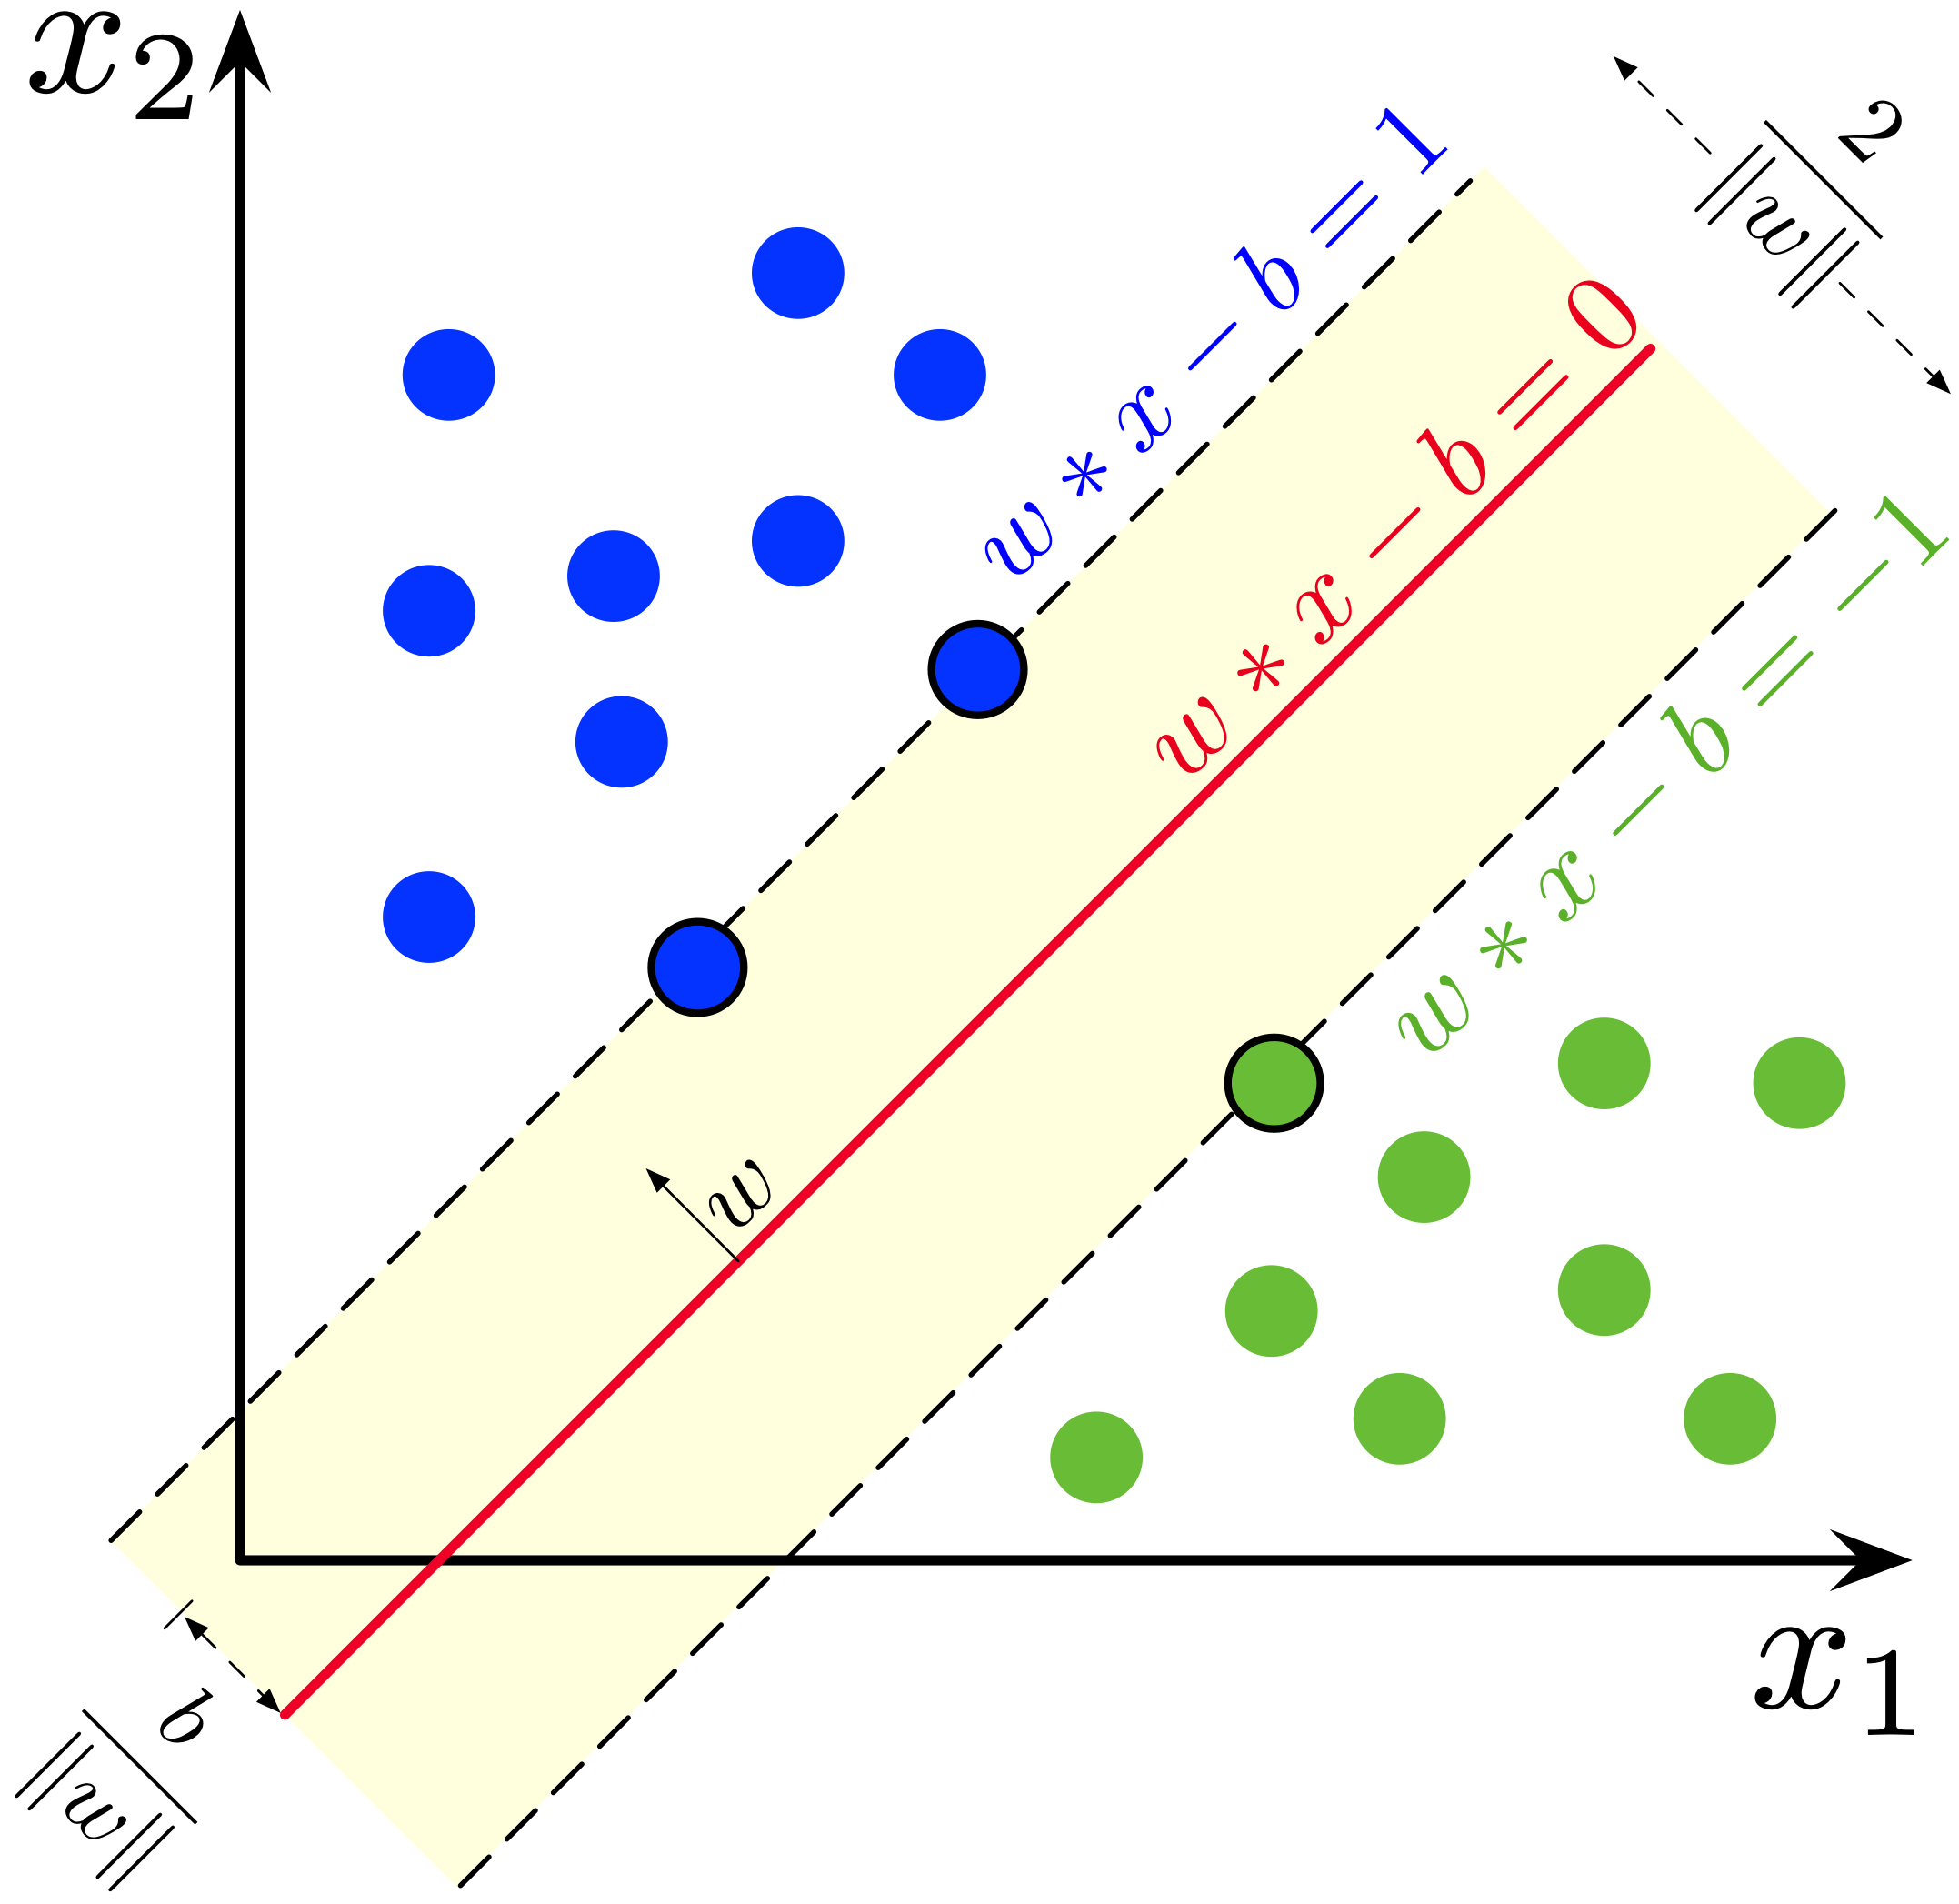
\includegraphics[width=0.5\textwidth]{images/svm-margin.png}
    \centering
    \caption{Maximum-margin hyperplane and margin for an \gls{svm} trained on two classes \cite{svm-margin}.}
    \label{fig:svm}
\end{figure}

The primary tunable parameters of a \glsxtrshort{svm} are \cite{scikit-svr,svr}:
\begin{itemize}
    \item Kernel function - determines the type of decision boundary. 
    \item Kernel hyperparameters - degree ($d$) for the polynomial kernel, gamma ($\gamma$) for the \glsxtrshort{rbf}, polynomial and sigmoid kernels and Gamma ($\gamma$) and intercept ($r$) for the polynomial and sigmoid kernels.
    \item Regularization strength ($C$) - controls the trade-off between maximizing the margin and minimizing the training error.
    \item Loss function - hinge loss for \glsxtrshort{svm} classification and $\varepsilon$-insensitive loss for \glsxtrshort{svr}.
    \item Epsilon-insensitive margin ($\varepsilon$) - margin of tolerance where no penalty is associated in the training loss function.
\end{itemize}

\subsubsection{Decision tree}\label{Decision tree}

\Glspl{dt} are a non-parametric supervised learning algorithm which is used for both classification and regression tasks. They have a hierarchical recursive partitioning structure which consists of a root node, branches, internal nodes and leaf nodes. The advantages of \glsxtrlong{dt} are that they are easy to interpret, require little to no data preparation and are robust to outliers. Their disadvantages are that they are prone to overfitting, susceptible to large structural changes caused by small variations in the data and more costly than other similar techniques. Their learning strategy involves searching for optimal dataset splits using information gain or entropy based splitting criteria including the Gini impurity or Shannon entropy measures \cite{prediction,ibm-dt}.

\subsubsection{Random forest}\label{Random forest}

\Glsxtrlongpl{rf} are an instance of ensemble learning techniques. Ensemble learning involves the aggregate use of more than one model in order to produce better results \cite{ibm-ensemble}. The base unit of a \glsxtrlong{rf} is a \glsxtrlong{dt}. A large number of \glsxtrlongpl{dt} is trained and evaluated on different subsets of the data obtained from different splits of the training set. Initial randomization is done via bootstrap samples drawn from the training set with replacement. Further randomization is then added via feature bagging which selects random subsets of features. The final output of the model is the majority vote or average of the outputs of all the trees. The biggest advantages of \glsxtrlong{rf} are a reduced risk of overfitting and the easy determination of feature importance. Their greatest disadvantages are a more resource intensive and time consuming process of model training due to the use of multiple models and greater model complexity \cite{prediction, ibm-rf}.

The primary tunable parameters of a \glsxtrlong{rf} are \cite{prediction,ibm-rf}:
\begin{itemize}
    \item The number of trees.
    \item The maximum number of features to consider at each split.
    \item Splitting criterion - based on impurity measures such as Shannon Entropy or Gini impurity.
\end{itemize}

\subsection{The foreign exchange market}\label{The foreign exchange market}

The \gls{forex} market is the largest liquid financial market in the world. It is a global \gls{otc} market (there is no central market place or exchange) closest to the ideal of perfect competition. It operates 24 hours a day 5 days a week and allows banks, businesses, investment firms, hedge funds, retail traders and individuals to buy, sell and exchange currencies \cite{forex}.

\subsection{Exchange rate prediction}\label{Exchange rate prediction}

Since the fall of the Bretton Woods system of fixed exchange rates in 1976 and the establishment of floating exchange rates with the Jamaica Accords, the need for accurate forecasting of exchange rates has become increasingly important. The primary reason for this is the need for effective risk management. Knowing whether the value of a currency will rise or fall ahead of time allows not only for the mitigation of adverse currency movements, but also for well-timed and potentially highly profitable investment decisions \cite{lstm-mlp-rf,deep-learning}.

According to the \gls{emh} \cite{efficient-market-hypothesis} financial markets are efficient and their prices reflect all information available at a given point in time. An implication of this is the inability to predict future prices on the basis of historical values. As such proponents argue that market prices follow a \gls{rw} where price movements are random and independent from one another. However this hypothesis is highly contested and numerous papers have shown that currency markets exhibit inefficiencies resulting in a delay between information availability and price adjustment \cite{adaptive-markets,event-study-analysis}.

Unfortunately, even so exchange rates are notoriously difficult to predict and rarely outperform a \gls{rw} model. They exhibit a complex non-linear nature that is dependant on a wide range of variables including macroeconomic and microeconomic factors \cite{factors}.  As such there is no single model that performs well for all combinations of predictors, forecast horizons, sample periods, forecasting evaluation methods and exchange rates. At short horizons (days, weeks, months) the fluctuations of the exchange rates are significantly greater and harder to predict. At longer horizons (years) various models have been proven to be able to make predictions better than the \gls{rw} \cite{predictability}.

Given the challenges in forecasting exchange rates using traditional econometric models, in recent years researchers have increasingly turned to the application of \gls{ai} algorithms as a potential solution.


\include{3-literature-review}
\section{Experimental setup}\label{Experimental setup}

A concise description of the computing environment used for the experiments is given below. First the hardware platform is summarised, followed by the software stack required for data‑processing, training and evaluation.

\subsection{Hardware specifications}\label{Hardware specifications}

The experiments were conducted on a standard Intel NUC workstation running NixOS.

\begin{table}[h!]
    \centering
    \caption{Core hardware parameters}
    \label{tab:hardware-specs}
    \begin{tabular}{|l|l|}
        \hline
        \textbf{Component} & \textbf{Value} \\
        \hline
        \hline
        Operating system & NixOS 25.11 (Xantusia) \\
        \hline
        Kernel & 6.18.8 \\
        \hline
        Host & Intel NUC8v5PNB \\
        \hline
        \Glsxtrshort{cpu} & Intel i5‑8365U (8 cores) @ 4.1 GHz \\
        \hline
        \Glsxtrshort{gpu} & Intel UHD Graphics 620 \\
        \hline
        \Glsxtrshort{ram} & 16 GiB \\
        \hline
    \end{tabular}
\end{table}

\subsection{Software stack}\label{Software stack}

All data‑preprocessing, model training and evaluation were performed with Python 3 and the open‑source libraries listed below.  Exact library versions are provided in table \ref{tab:software-versions} to support reproducibility.

\begin{table}[h!]
    \centering
    \caption{Software versions used in the study}
    \label{tab:software-versions}
    \begin{tabular}{|l|l|}
        \hline
        \textbf{Package} & \textbf{Version} \\
        \hline
        \hline
        Python & 3.13.11 \\
        \hline
        NumPy & 2.3.4 \\
        \hline
        pandas & 2.3.1 \\
        \hline
        scikit‑learn & 1.7.1 \\
        \hline
        statsmodels & 0.14.5 \\
        \hline
        Optuna & 4.8.0 \\
        \hline
        pmdarima & 2.1.1 \\
        \hline
    \end{tabular}
\end{table}

\subsubsection*{Python 3}

%The programming language used in all steps of this research paper was Python. The primary reason for this was its simple but powerful syntax wide spread use, the broad availability of various libraries and frameworks for data processing, analysis and \gls{ai} modeling including scikit-learn, keras and pytorch among many others as well as the associated availability of information on the use of these various tools provided by the extensive community surrounding them \cite{python}.

The primary programming language; chosen for its readability, large ecosystem and extensive community support \cite{python}.

\subsubsection*{NumPy}

% A python package for accelerated array based scientific computing utilizing a C based backend implementation with various optimizations \cite{numpy}.

A high‑performance array library with a C backend for scientific computing \cite{numpy}.

\subsubsection*{pandas}

% A python software library for data manipulation and analysis \cite{pandas}.

A data‑manipulation and analysis toolkit for tabular data \cite{pandas}.

\subsubsection*{scikit‑learn}

% A python library for the training and verification of machine learning models for predictive data analysis \cite{scikit-learn}.

A collection of algorithms for training and validating machine‑learning models \cite{scikit-learn}.

\subsubsection*{statsmodels}

% A python module for the estimation of many different statistical models, conducting statistical tests and statistical data exploration \cite{statsmodels}.

Provides statistical model estimation, tests and exploratory tools \cite{statsmodels}.

\subsubsection*{Optuna}

% An automatic hyperparameter optimization software framework, particularly designed for machine learning. It features an imperative, define-by-run style user API \cite{optuna}.

Framework for automatic hyper‑parameter optimisation using a define‑by‑run API \cite{optuna}.

\subsubsection*{pmdarima}

% A statistical library for time series analysis and forecasting \cite{pmdarima}.

Statistical library specialised in time‑series analysis and forecasting \cite{pmdarima}.


\section{Data preparation}\label{Data preparation}

In this paper data preparation for use in \gls{ai} model creation consists of two steps: acquisition and preprocessing.

\subsection{Acquisition}\label{Acquisition}

The data chosen for this study was a set of \gls{cpi}-deflated \gls{eer} obtained from the website of the \gls{ecb} \cite{forex-data}. The data consists of three sets of deflated \gls{eer} one on the basis of a group of 13 currencies, one 18 currencies and one 41 currencies. The data is sampled at a monthly frequency and covers the time frame from the 31.01.1993 to 31.10.2025. The currencies included in the dataset are: \gls{aed}, \gls{ars}, \gls{aud}, \gls{bgn}, \gls{brl}, \gls{cad}, \gls{chf}, \gls{clp}, \gls{cny}, \gls{cop}, \gls{czk}, \gls{dkk}, \gls{dzd}, \gls{eur}, \gls{gbp}, \gls{hkd}, \gls{huf}, \gls{idr}, \gls{ils}, \gls{inr}, \gls{isk}, \gls{jpy}, \gls{krw}, \gls{mad}, \gls{mxn}, \gls{myr}, \gls{nok}, \gls{nzd}, \gls{pen}, \gls{php}, \gls{pln}, \gls{ron}, \gls{rub}, \gls{sar}, \gls{sek}, \gls{sgd}, \gls{thb}, \gls{try}, \gls{twd}, \gls{uah}, \gls{usd}, \gls{zar}.

\subsection{Required preprocessing steps}\label{Required preprocessing steps}

The cleaning and preparation of the data was conducted in order to increase the accuracy of predictions as well as improve the efficiency of model training.

\subsubsection{Handling of missing values}\label{Handling of missing values}

The handling of missing values consisted of the removal of variables with more than two sequential variable specific missing values, caused by insufficient market activity and reporting inconsistencies, of which there was 1 (41-RUB), leaving behind 73 currency exchange rates. This step was crucial, as missing data can lead to biased estimates and can negatively affect the overall performance of predictive models \cite{techniques,rf-svr}.

\subsection{Optional intermediary steps}\label{Optional intermediary steps}

\subsubsection{Log transformation}\label{Log transformation}

In this step a natural logarithm transformation of the data was applied in order to stabilize the variance and prevent heteroscedacity \cite{nn-vs-chaotic,robust-regression,gbp-usd-forecasting}.

\subsubsection{Differencing}\label{Differencing}

In this step first-order differencing was applied to the dataset. This procedure causes the replacement of successive values with successive variations. This is a necessary step in the preparation of the data enabling the removal of trends, seasonality, and other non-stationary components from the original time series \cite{nn-vs-chaotic,robust-regression,gbp-usd-forecasting}.

\begin{figure}[h!]
    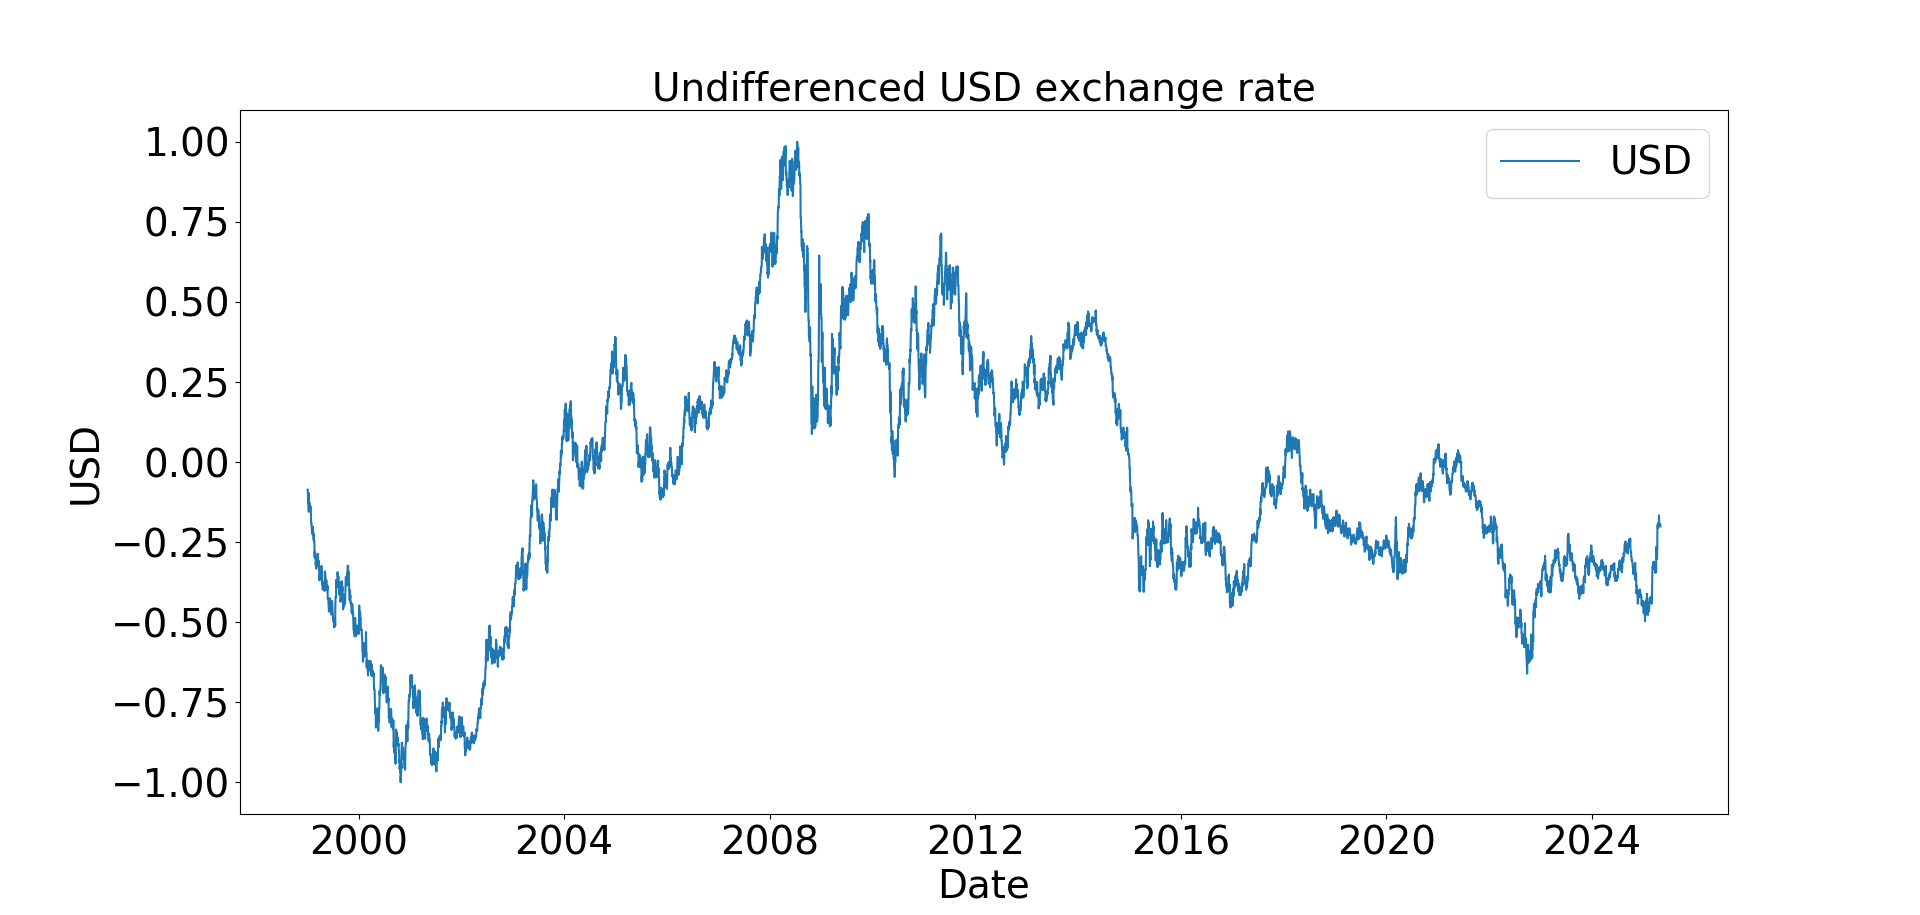
\includegraphics[width=\textwidth]{images/preprocessing/3-optional/differencing/usd-undiff.png}
    \centering
    \caption{The undifferenced forward filled \gls{usd} spot exchange rate.}
    \label{fig:usd-undiff}
\end{figure}

\begin{figure}[h!]
    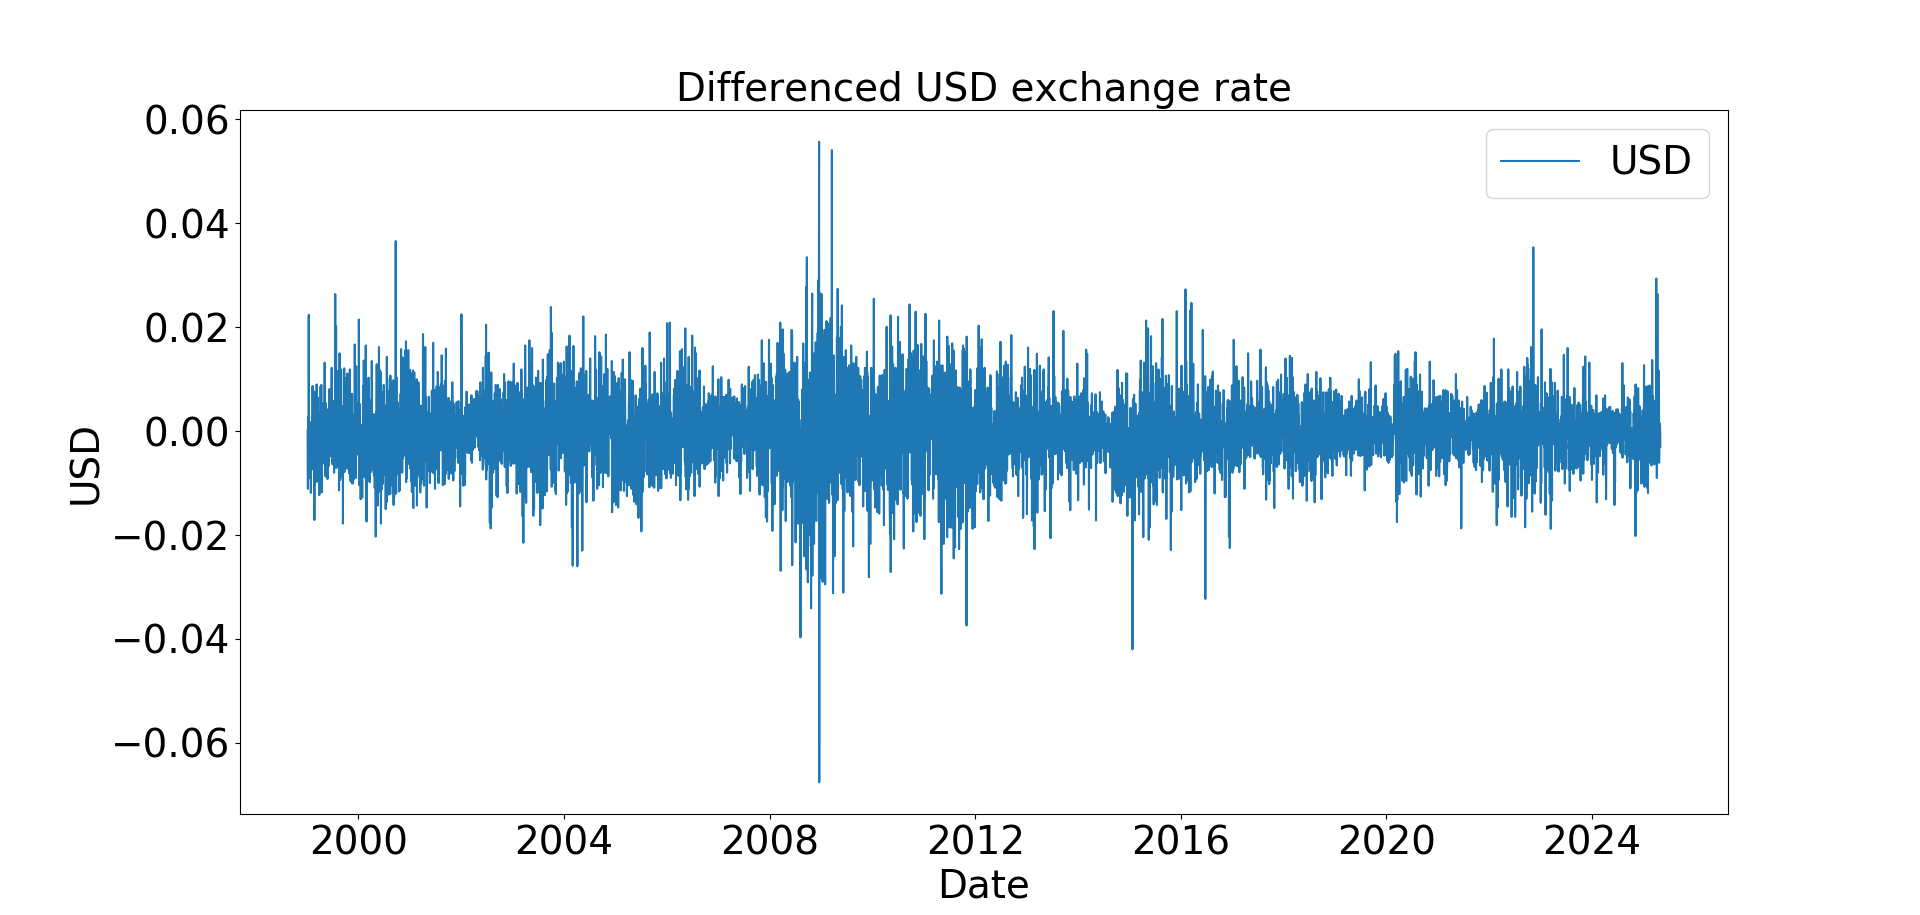
\includegraphics[width=\textwidth]{images/preprocessing/3-optional/differencing/usd-diff.png}
    \centering
    \caption{The differenced \gls{usd} spot exchange rate.}
    \label{fig:usd-diff}
\end{figure}

\subsubsection{Feature scaling}\label{Feature scaling}

Feature scaling is an essential step in the data preparation for many \gls{ai} models which often exhibit better training efficiency and forecasting accuracy with scaled data. This is especially true for \gls{mlp} and \gls{svr}. For the \gls{rf} machine learning model this step is not required due to insensitivity and as a result has been omitted. Two feature scaling methods where used in the data preparation process for different models in this paper. An visual representation of the effects of both can be seen in figure \ref{fig:usd-scaling}.

\begin{itemize}
    \item Normalization via scikit-learn's MinMaxScaler \cite{scikit-learn} to the range [-1,1] was used in the preparation of data primarily for use with the \gls{mlp} with the \gls{tanh} activation function \cite{nn-vs-chaotic,ann-2}.
    \item Standardization via scikit-learn's StandardScaler \cite{scikit-learn} to a mean of zero and a variance of one was used primarily in the data preparation pipeline for use with \gls{svr} \cite{genetic,rf-svr}.
\end{itemize}

\begin{figure}[h!]
    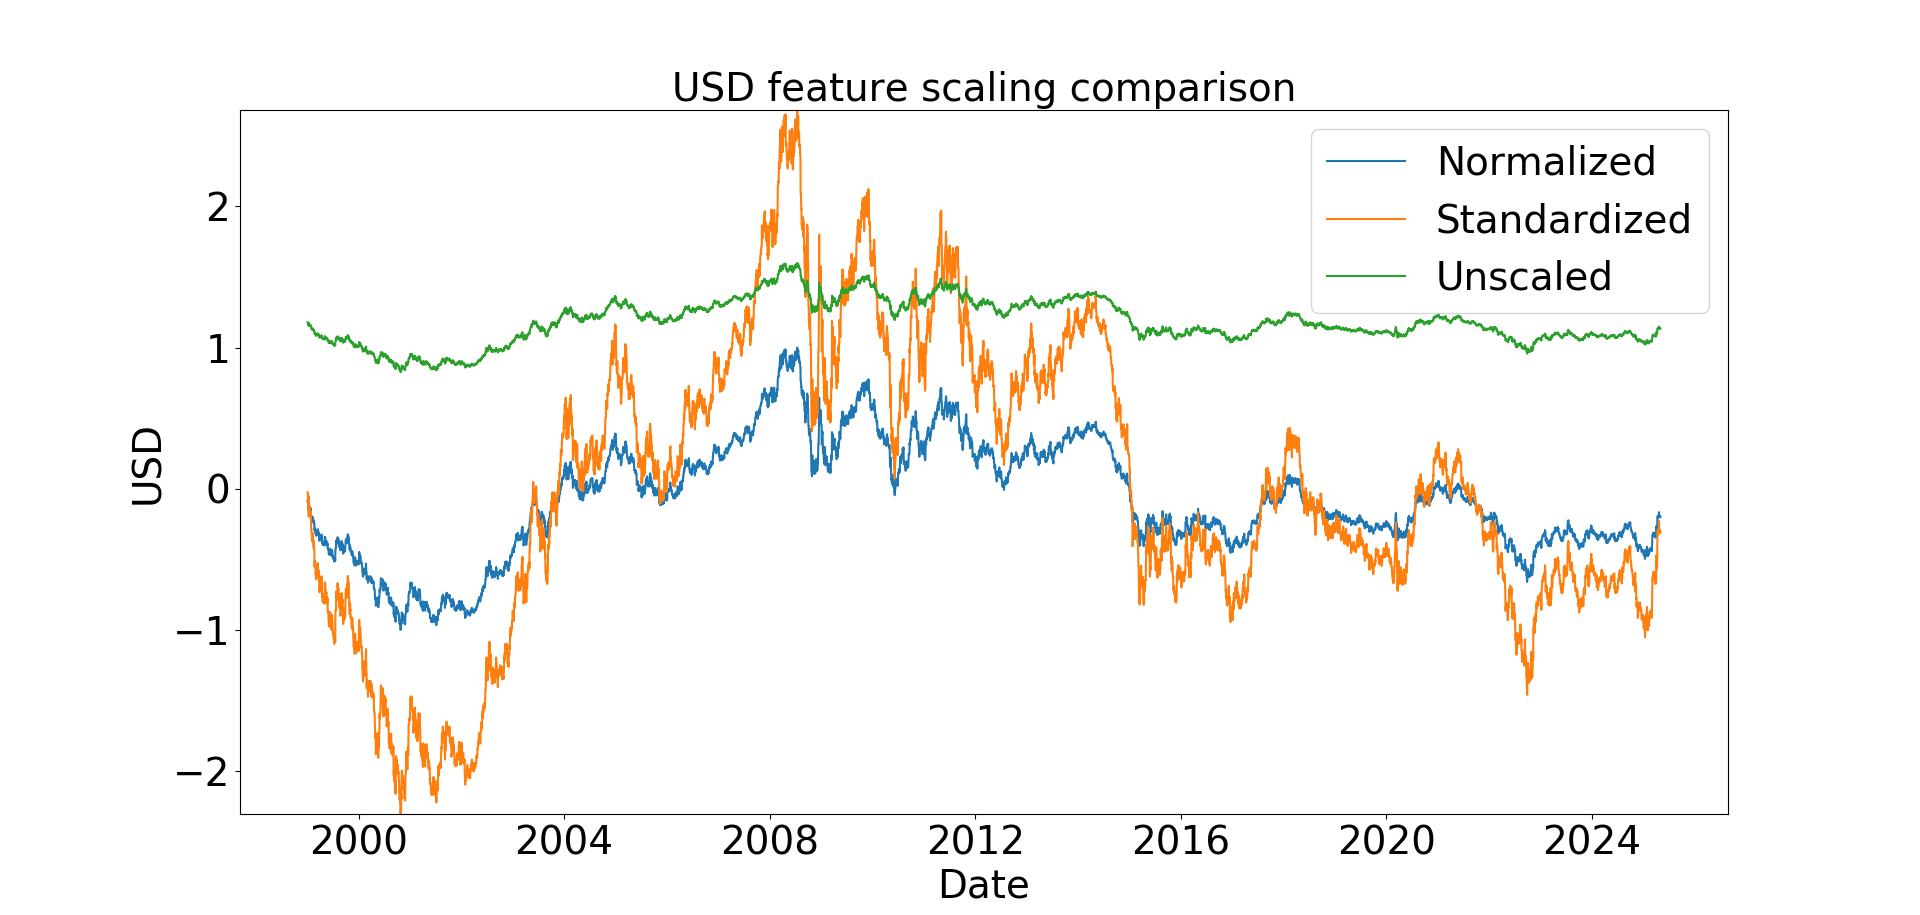
\includegraphics[width=\textwidth]{images/preprocessing/3-optional/scaling/usd-scaling.png}
    \centering
    \caption{A graphical comparison of normalization and standardization on the basis of the \gls{usd} spot exchange rate.}
    \label{fig:usd-scaling}
\end{figure}

\subsection{Required postprocessing steps}\label{Required postprocessing steps}

\subsubsection{Feature extraction}\label{Feature extraction}

For this step three different target variables were chosen each representing the \gls{usd} exchange rate for the different sized groupings of trading partners used for CPI-deflation. Time lagged versions of each dataset for each feature variable upto 12 months were created for each preprocessing variation \cite{rf-svr,gold}. An example of the shifting procedure for the \gls{usd} exchange rate is shown in figure \ref{fig:feature-extraction}.

\begin{figure}[h]
    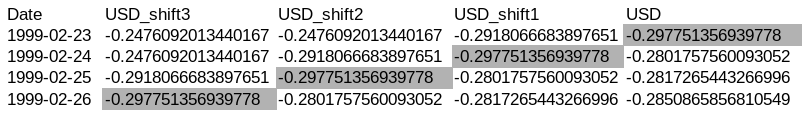
\includegraphics[width=\textwidth]{images/preprocessing/4-usd-shifts-3.png}
    \centering
    \caption{An example of a series of time shifts upto three days for the \gls{usd} exchange rate.}
    \label{fig:feature-extraction}
\end{figure}

% \subsubsection{Variable selection}\label{Variable selection}
% 
% In the next step scikit-learn's \gls{rfecv} \cite{scikit-learn} was used with the \gls{svr} model with a linear kernel as the estimator for feature importance ranking and optimal feature subset selection.
% 
% The \gls{cv} results for each dataset are presented in figure \ref{fig:rfecv}. As can be see the absence of scaling as well as in the case of scaling the chosen scaling methodology greatly affect the results of \gls{rfecv}.
% 
% For the \gls{mlp} dataset for which normalization was employed the optimal number of features selected by the \gls{rfecv} was 33.
% 
% For the \gls{svr} dataset for which standardization was employed the optimal number of features selected by the \gls{rfecv} was 9.
% 
% For the \gls{rf} dataset for which no scaling procedures were used the number of features selected by the \gls{rfecv} was 34.
% 
% \begin{figure}[h]
%     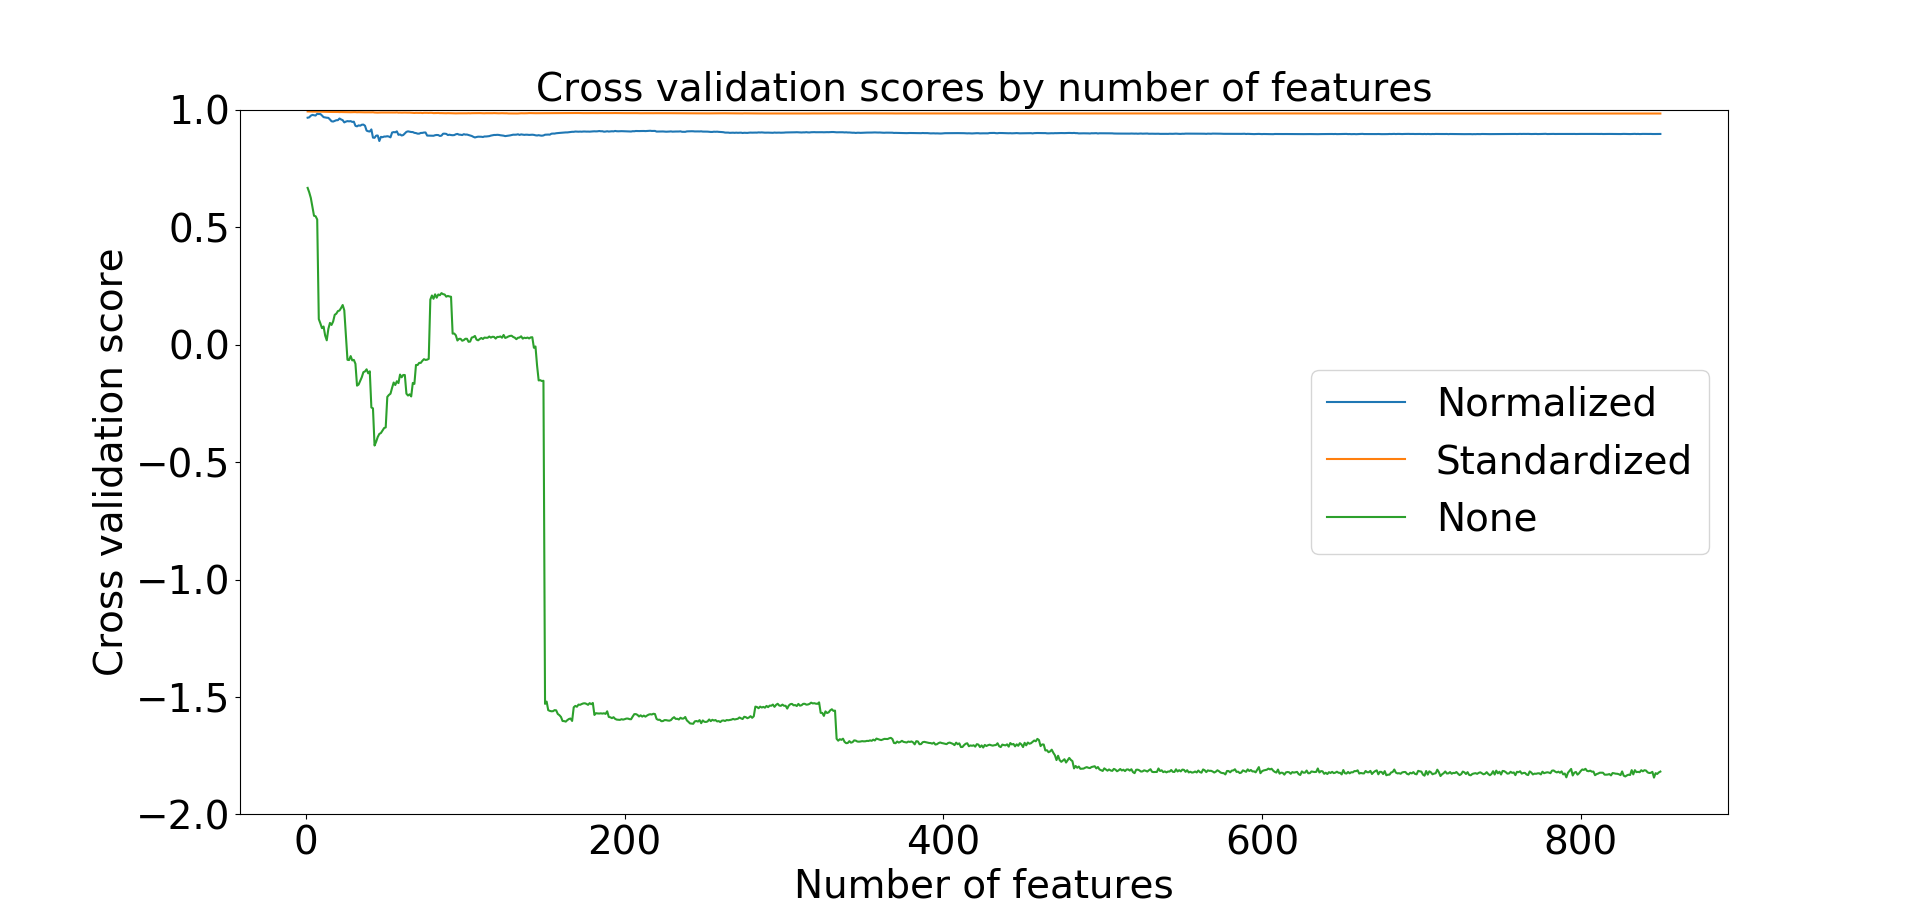
\includegraphics[width=\textwidth]{images/preprocessing/5-variable-selection/rfecv.png}
%     \centering
%     \caption{\Gls{cv} scores by number of features for normalized (\gls{mlp}), standardized (\gls{svr}) and unscaled (\gls{rf}) datasets.}
%     \label{fig:rfecv}
% \end{figure}

\subsubsection{Feature decorrelation}\label{Feature decorrelation}

In the next step a Pearson correlation matrix was constructed for the feature and target exchange rates to assess the linear relationships among them. Features exhibiting weak correlation $\le 0.1$ with the target were removed first, as they contribute noise without predictive signal. Next feature variables that had a high mutual correlation $\ge 0.9$ with at least one other feature were removed. This was done to mitigate the risk of multicollinearity, which can lead to the occurrence of amplifying or distorting effects during model training \cite{genetic}. As a result of this analysis, the initial feature set for each dataset processing variation was significantly reduced.

\subsubsection{Data split}\label{Data split}

For the purpose of model training and forecasting accuracy evaluation each dataset was split into two subsets with a separation strip equal to the degree of generated time lags (150) in order to prevent information leakage from the training set to the test set:
\begin{itemize}
    \item training $+$ validation (70\%) - for model training and k-fold cross-validation.
    \item testing (30\%) - for the final evaluation of the selected model in order to prevent overfitting and enable a unbiased evaluation of the model on new unseen data.
\end{itemize}


\section{Model training and evaluation}\label{Model training and evaluation}

This section presents an overview of the primary guiding principals used during the stages of model training and evaluation.

\subsection{Bias-Variance dilemma}\label{Bias-Variance dilemma}

The bias-variance dilemma is a fundamental problem in machine learning and involves the issues of model optimization and generalization. In the case of optimization (reducing the model error) a model eventually starts to overfit the training data, this results in high error of the models predictions on the test/validation datasets (high variance). The opposite is aiming to increase model generalization (reduction of model complexity) however this in turn causes underfitting or high error of the models predictions on the training dataset (high bias). This counterpoised behaviour of both bias and variance enables the easy assessment of model suitability for use in the prediction of unseen data \cite{ibm-ensemble,ibm-regularization,svm-2}.

% Juxtaposed
%
% In the case of generalization (reduction of model complexity) a model starts to underfit the training data, this results in high error of the models predictions on the training dataset (high bias).
%
% The opposite is aiming to increase model optimization (reducing the model error) however this in turn pushed to far causes overfitting or high error of the models predictions on the test/validation datasets (high variance).

\subsection{Performance metric}\label{Performance metric}

The accuracy of the model forecasts was evaluated on the basis of the \glsxtrlong{mse} this metric measures the average squared difference between predicted and actual values, providing a sense of the magnitude of the errors. A lower \gls{mse} indicates better fit, but it is sensitive to outliers due to the squaring of errors \cite{scikit-mse}.

$$MSE = \frac{1}{n} \sum_{i=1}^{n} (y_i - \hat{y}_i)^2$$

Where:
\begin{itemize}
    \item $n$ is the total number of predictions
    \item $y_i$ is the actual value at time $i$
    \item $\hat{y}_i$ is the predicted value at time $i$
\end{itemize}

\subsection{Methodology}\label{Methodology}

The process of model training and evaluation consisted of model fitting using the Optuna hyperparameter optimization framework with the goal of minimizing the \gls{mse} followed by data analysis of the obtained optized forecasts. During analysis for each model accuracy was evaluated on both in-sample (training set) and out-of-sample (test set) data. The preprocessing variant yielding the minimum average \gls{mse} across all offsets (train and test sets combined) was selected as optimal.

\subsubsection{Optuna model fitting}\label{Optuna model fitting}

In the first step each of the models was fitted on different suitable dataset processing variations. For the purpose of efficient and reproducible hyperparameter optimization that exceeds what can be achieved within reasonable time frames using the GridSearchCV class from scikit-learn, an alternative drop-in replacement class OptunaSearchCV provided by the Optuna package was used instead. Unlike grid search's exhaustive enumeration, Optuna's \gls{tpe} sampler efficiently explores the hyperparameter space through Bayesian optimization, focusing computational effort on promising regions of the hyperparameter space. For the \gls{mlp} only datasets for which normalization was applied as the last step were used. For the \gls{rf} all dataset processing variations were evaluated. For \gls{svr} only datasets processing methods that ended with standardization were used.

Beyond the parameters being optimized each model was used with its default parameters with some exceptions. For the \gls{mlp} the activation function was changed to \gls{tanh} due to the normalization range of the data, shuffle was set to false to prevent data shuffling in order to not disrupt the continuous time series nature of the data, random state was set to zero for reproducability of the results and the maximum number of iterations was increased to 10000 in order to allow for model convergence. For the \gls{rf} only the random state was set. For the \gls{svr} non of the default parameters were changed.

The parameters being optimized via OptunaSearchCV for each model as well as their selected value distributions are presented in table \ref{tab:mlp-hyperparams} for \gls{mlp}, table \ref{tab:rf-hyperparams} for \gls{rf}, table \ref{tab:svr-hyperparams} for \gls{svr} and table \ref{tab:arima-hyperparams} for \gls{arima}. The variable ranges were selected through manual experimentation to be broad and provide an ample search space for optimization.

OptunaSearchCV was run for 1000 iterations for each model for each applicable dataset variation for each offset from 1 to 12 months. All parameters were retained at default values other than 'scoring' which was set to 'neg\_mean\_squared\_error'.

\begin{table}[h]
    \centering
    \caption{Optuna hyperparameter search space for MLPRegressor}
    \begin{tabular}{|c|c|}
        \hline
        Parameter & Distribution \\
        \hline
        \hline
        hidden\_layer\_sizes & $Int(1, 30)$ \\
        \hline
        alpha & $Float(10^{-10}, 10^{-1})$ \\
        \hline
        tol & $Float(10^{-8}, 10^{-1})$ \\
        \hline
    \end{tabular}
    \label{tab:mlp-hyperparams}
\end{table}

\begin{table}[h]
    \centering
    \caption{Optuna hyperparameter search space for RandomForestRegressor}
    \begin{tabular}{|c|c|}
        \hline
        Parameter & Distribution \\
        \hline
        \hline
        n\_estimators & $Int(1, 40)$ \\
        \hline
        max\_depth & $Int(1, 40)$ \\
        \hline
        max\_features & $Int(1, 44)$ \\
        \hline
    \end{tabular}
    \label{tab:rf-hyperparams}
\end{table}

\begin{table}[h]
    \centering
    \caption{Optuna hyperparameter search space for SVR}
    \begin{tabular}{|c|c|}
        \hline
        Parameter & Distribution \\
        \hline
        \hline
        tol & $Float(10^{-6}, 10^{-1})$ \\
        \hline
        C & $Int(100, 2000)$ \\
        \hline
        $\epsilon$ & $Float(10^{-8}, 10^{-1})$ \\
        \hline
    \end{tabular}
    \label{tab:svr-hyperparams}
\end{table}

\begin{table}[h]
    \centering
    \caption{Optuna hyperparameter search space for ARIMA}
    \begin{tabular}{|c|c|}
        \hline
        Parameter & Distribution \\
        \hline
        \hline
        p & $Int(0, 6)$ \\
        \hline
        d & $Int(0, 6)$ \\
        \hline
        q & $Int(0, 6)$ \\
        \hline
    \end{tabular}
    \label{tab:arima-hyperparams}
\end{table}

\subsubsection{Data analysis}\label{Data analysis}

The forecasts obtained in the previous step were reverse transformed to obtain values in the same range as those of the original \gls{eer}. This was done due to the scale dependant nature of the \gls{mse} metric. Next for each dataset variation the cumulative averages for all offsets of the average \gls{mse} for both the training and test set forecasts were calculated.

% Step not intended for:
% - Comparing the MSE vs Hitrate not viable
% - Comparing models not viable

% Step intended for:
% - Comparing the results for various dataset preprocessing steps for each model in order to find best dataset processing variant
% - Basic trend observation

% General notes:
% - Models were optimized by MSE not Hitrate
% - Possible trends for description: best to worst

% Observations by case:
% - \gls{arima} \gls{mse}
%     + Best ld
%     + Worst ld that had been additionally scaled either via standardization of normalization.
%     + The best variation had a significantly smaller error than any other dataset variation
%     + The worst two ldn and lds had a significantly greater error than the rest of the dataset processing variations
%
% - \gls{arima} \gls{ds}
%     + The difference in \gls{ds} between the various dataset varients was not significant
% - \gls{mlp} \gls{mse}
% - \gls{mlp} \gls{ds}
% - \gls{rf} \gls{mse}
% - \gls{rf} \gls{ds}
% - \gls{svr} \gls{mse}
% - \gls{svr} \gls{ds}


As a result multiple rankings were obtained which can be seen in figure \ref{fig:mlp-mse} for \gls{mlp}, figure \ref{fig:rf-mse} for \gls{rf}, figure \ref{fig:svr-mse} for \gls{svr} and figure \ref{fig:arima-mse} for \gls{arima}. For the \gls{rw} model only the raw data was used.

% Bar charts for the average MSE and Hitrate for different dataset variations for each model

\begin{figure}[h]
    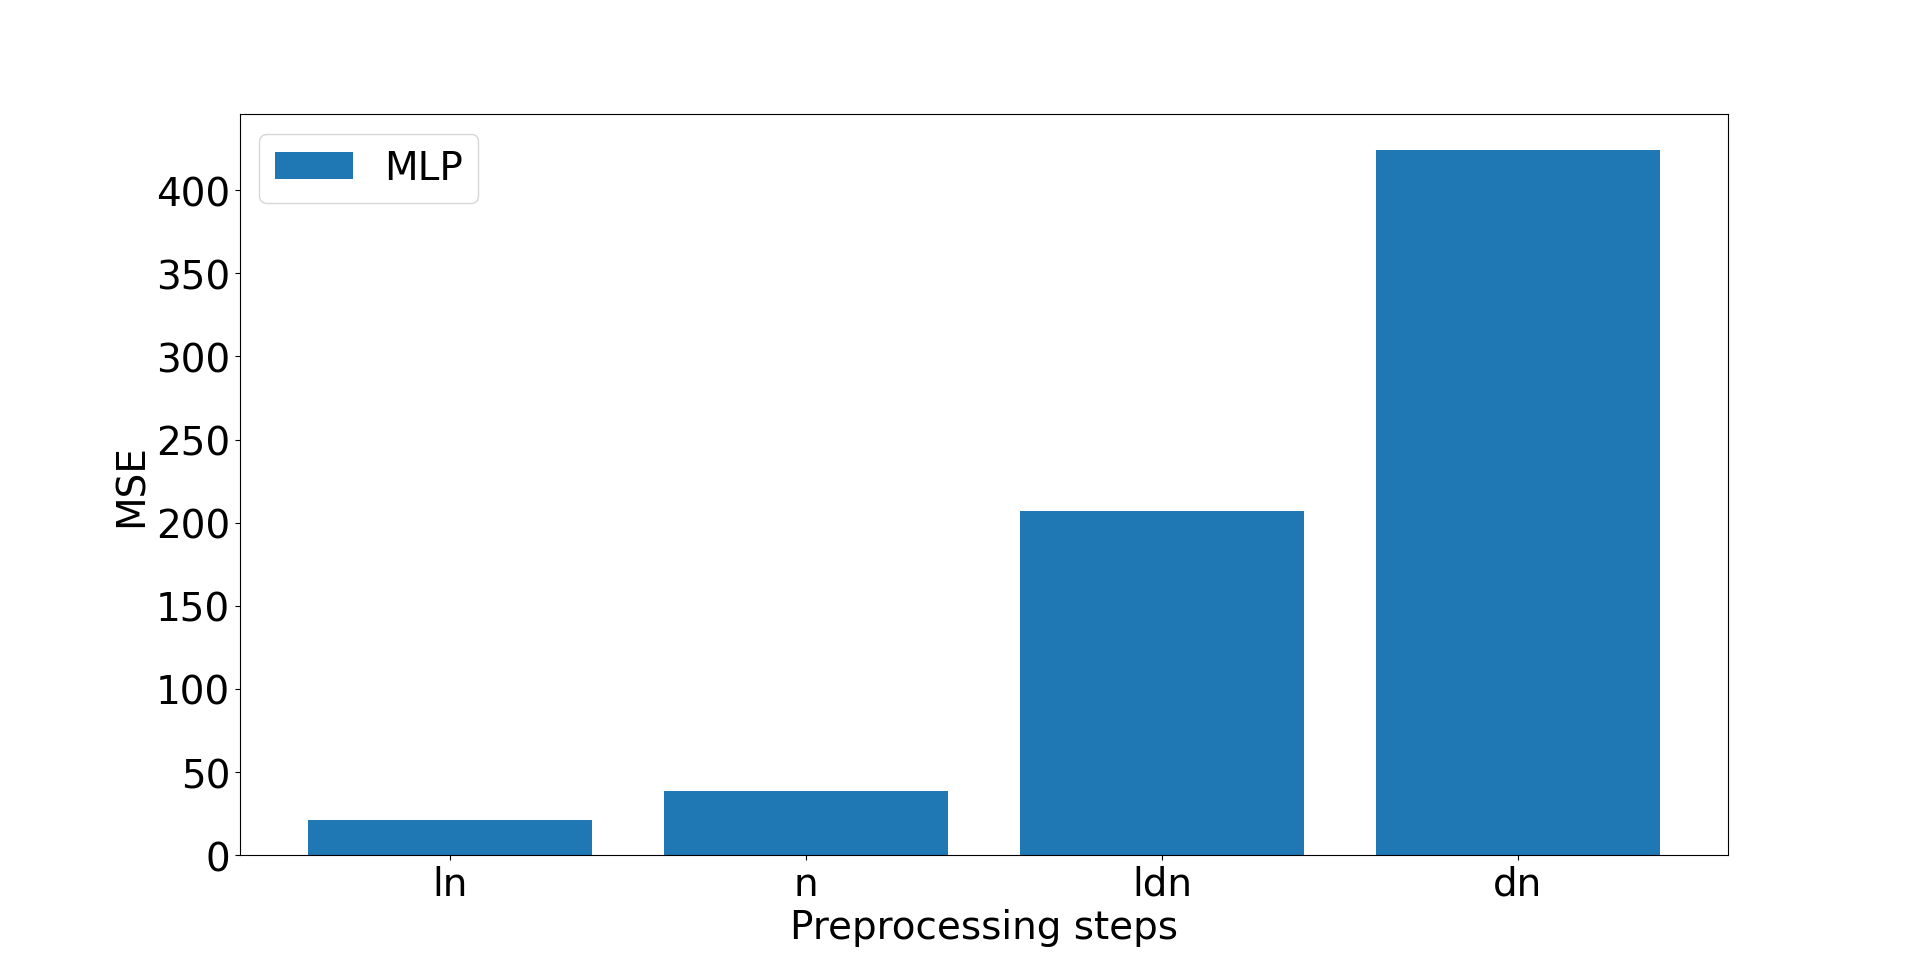
\includegraphics[width=\textwidth]{images/metrics-by-dataset/mlp_mse.png}
    \centering
    \caption{The \gls{mse} for the \gls{mlp} model for various preprocessing steps. The sets of processing steps are indicated in shorthand as follows: l - log transformed, d - differenced, n - normalized.}
    \label{fig:mlp-mse}
\end{figure}

\begin{figure}[h]
    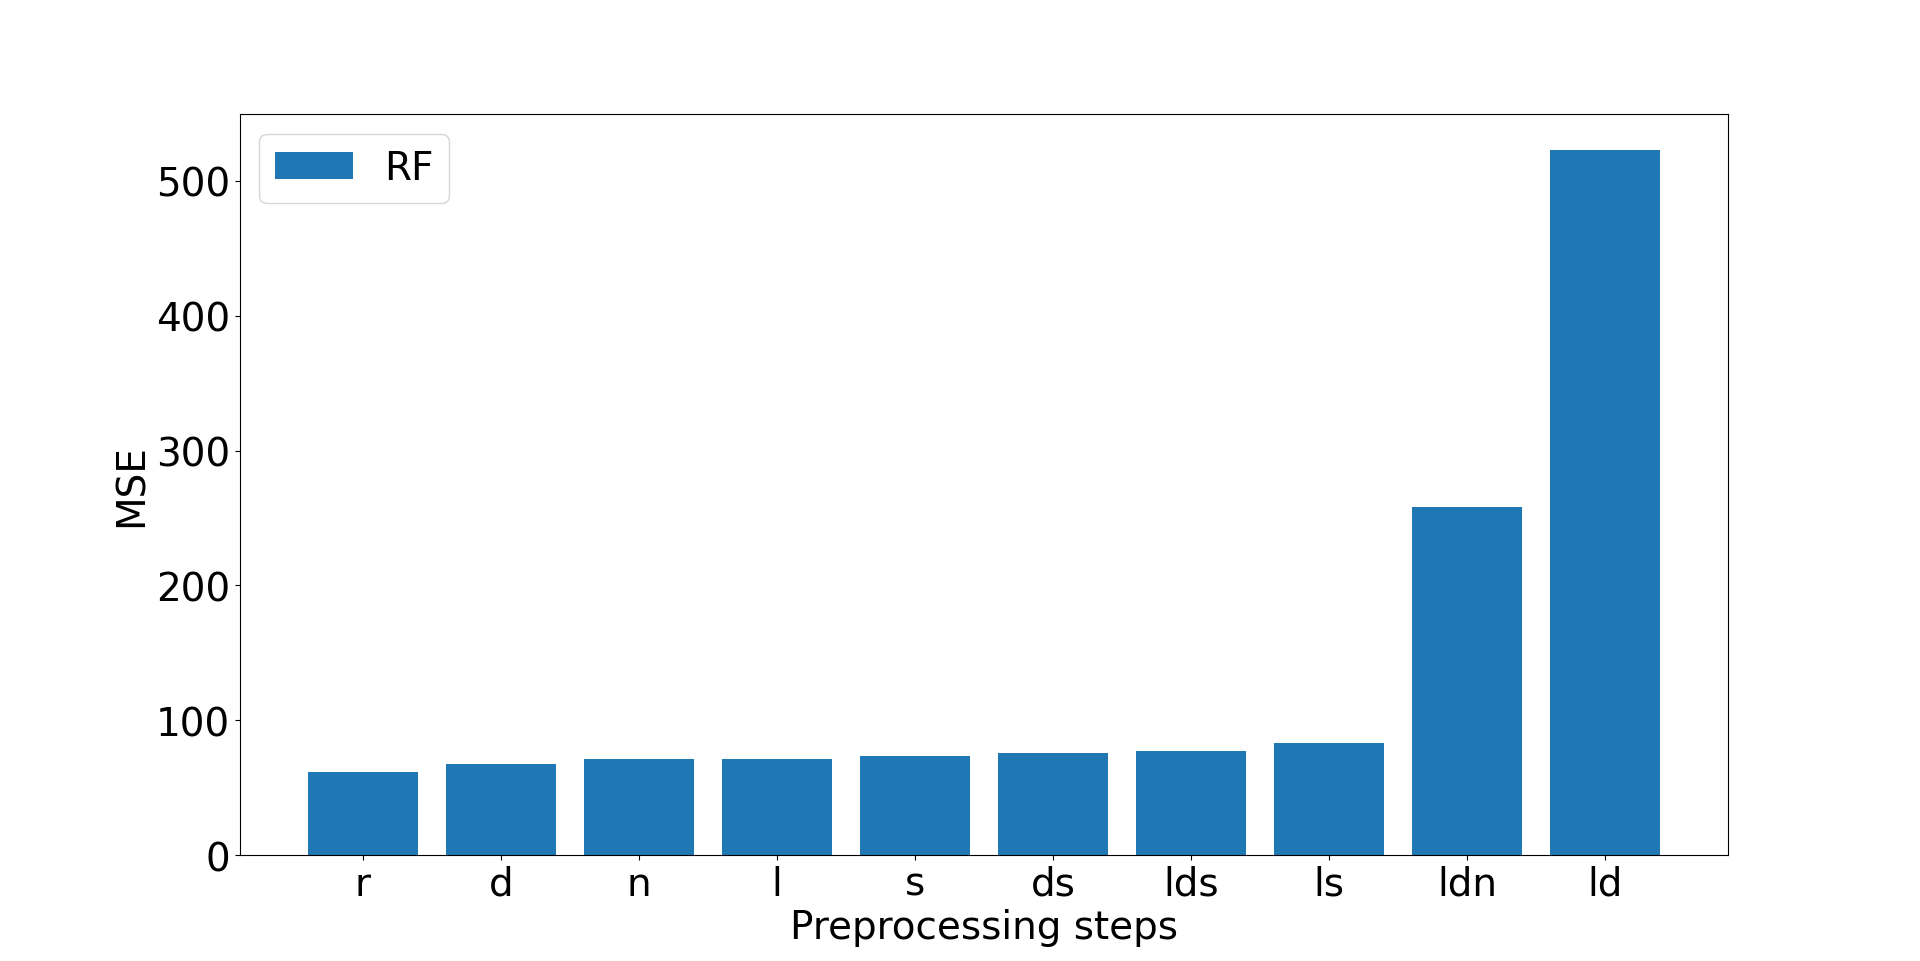
\includegraphics[width=\textwidth]{images/metrics-by-dataset/rf_mse.png}
    \centering
    \caption{The \gls{mse} for the \gls{rf} model for various preprocessing steps. The sets of processing steps are indicated in shorthand as follows: l - log transformed, d - differenced, n - normalized, s - standardized, r - raw.}
    \label{fig:rf-mse}
\end{figure}

\begin{figure}[h]
    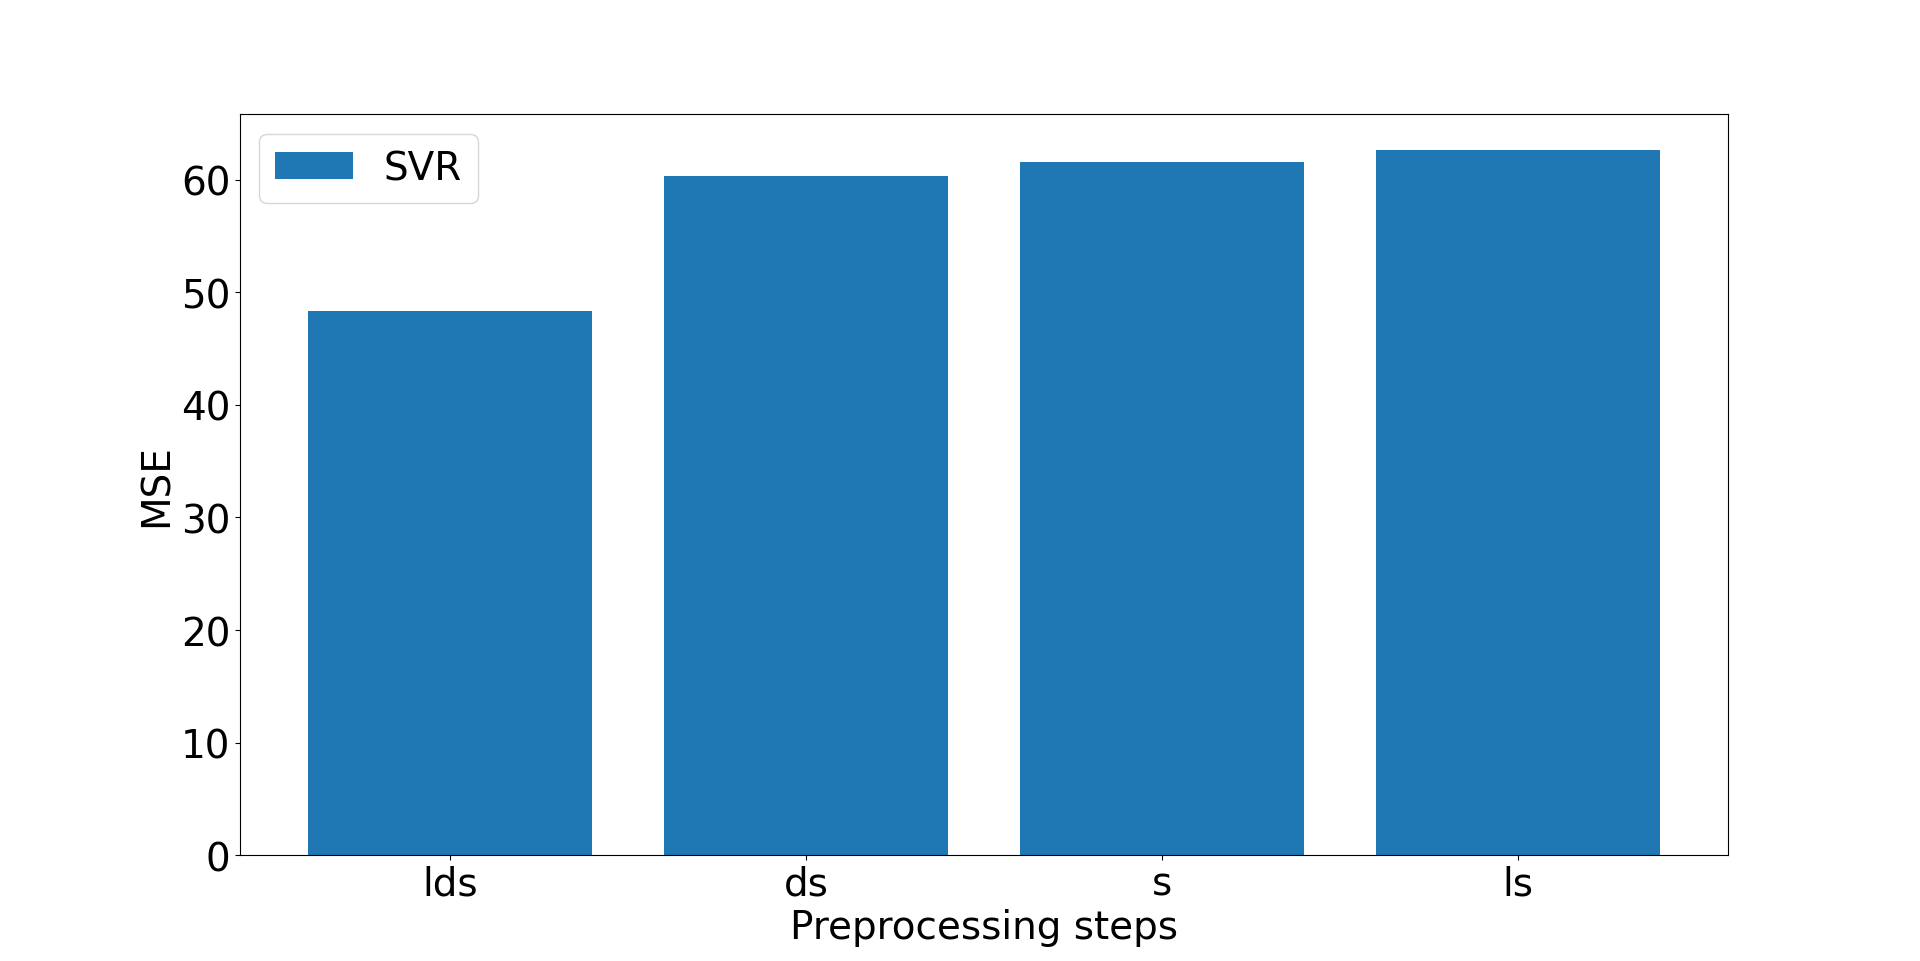
\includegraphics[width=\textwidth]{images/metrics-by-dataset/svr_mse.png}
    \centering
    \caption{The \gls{mse} for the \gls{svr} model for various preprocessing steps. The sets of processing steps are indicated in shorthand as follows: l - log transformed, d - differenced, s - standardized.}
    \label{fig:svr-mse}
\end{figure}

\begin{figure}[h]
    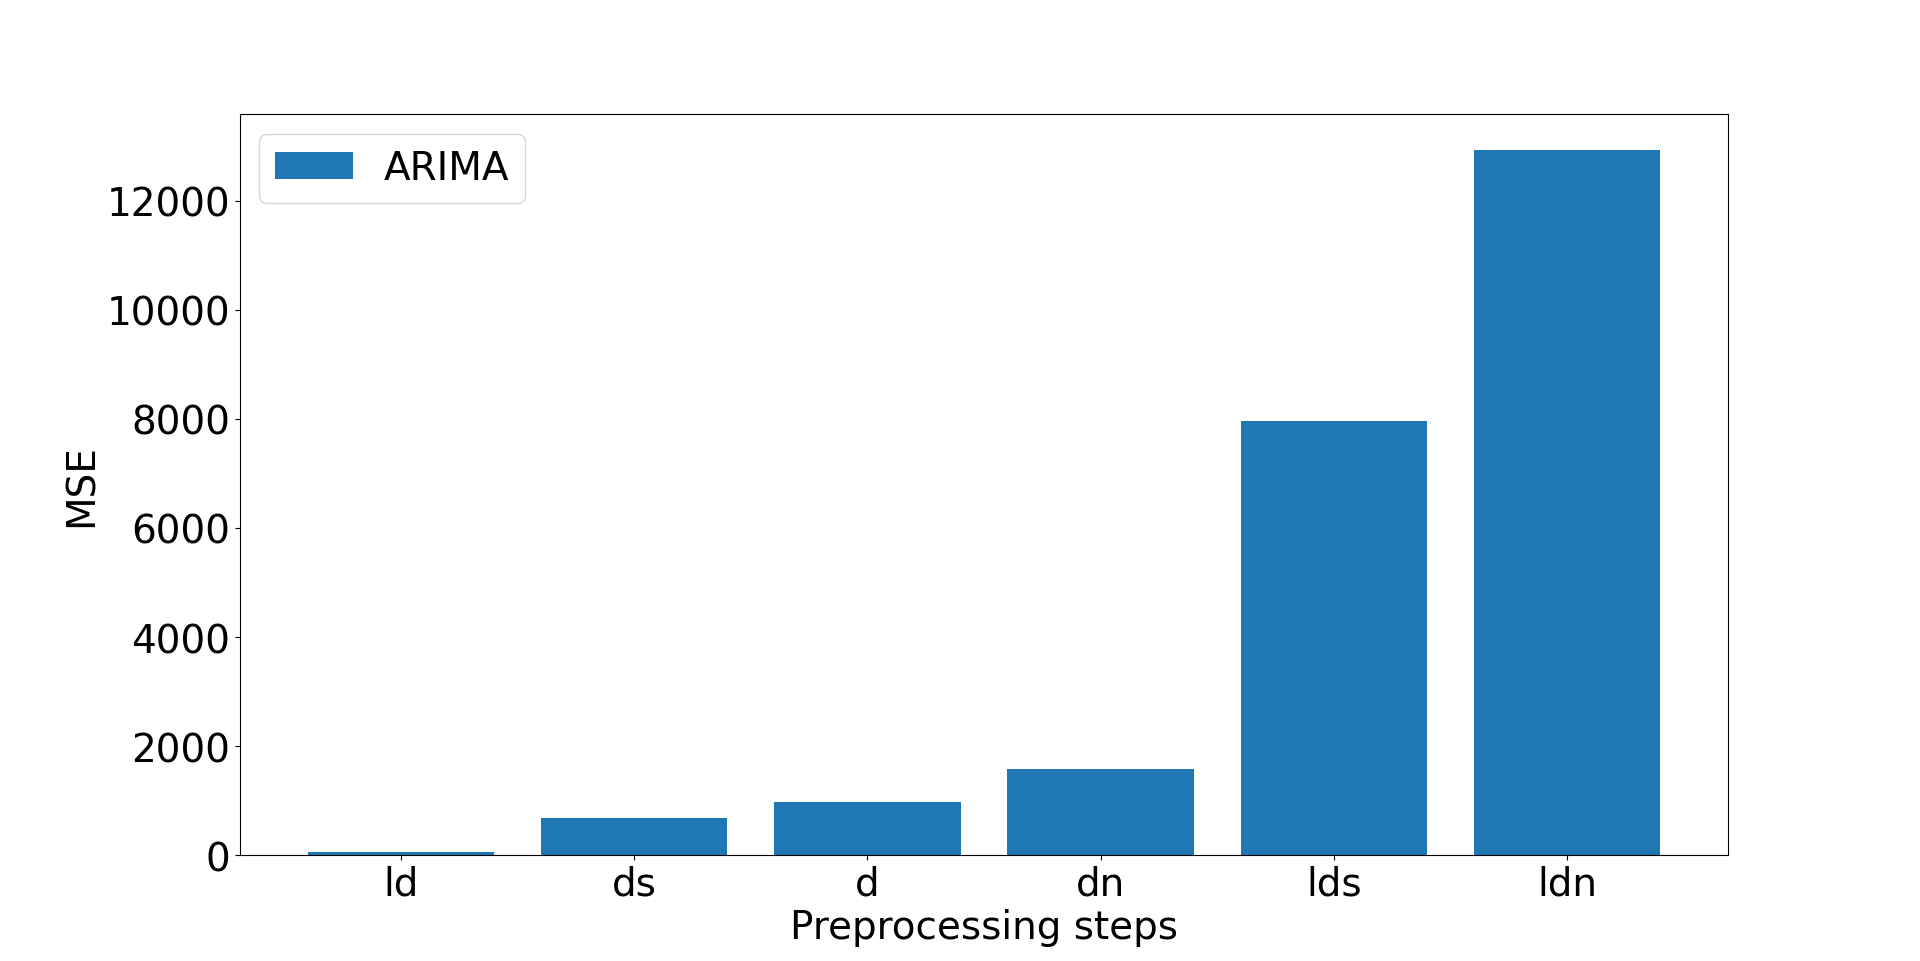
\includegraphics[width=\textwidth]{images/metrics-by-dataset/arima_mse.png}
    \centering
    \caption{The \gls{mse} for the \gls{arima} model for various preprocessing steps. The sets of processing steps are indicated in shorthand as follows: l - log transformed, d - differenced, n - normalized, s - standardized, r - raw.}
    \label{fig:arima-mse}
\end{figure}

On the basis of the created rankings the best dataset preprocessing variations for each model were selected. The results are displayed in table \ref{tab:best-datasets}.

% Metric - Model - Preprocessing steps
% mse - mlp - log-normalized
% hitrate - mlp - log-diff-normalized
% mse - rf - raw
% hitrate - rf - log-transformed
% mse - svr - log-diff-standardized
% hitrate - svr - log-diff-standardized

\begin{table}[h]
    \centering
    \caption{The best dataset preprocessing steps per model by \gls{mse}.}
    \begin{tabular}{|c|c|}
        \hline
        Model & Preprocessing Steps \\
        \hline
        \hline
        \gls{mlp} & log-normalized \\
        \hline
        \gls{rf} & raw \\
        \hline
        \gls{svr} & log-diff-standardized \\
        \hline
        \gls{arima} & log-differenced \\
        \hline
    \end{tabular}
    \label{tab:best-datasets}
\end{table}

\newpage

For the purpose of comparing the overall performance of different models the average \gls{mse} over both the train and test sets over all offsets was calculated. The results are visible in the bar chart in figure \ref{fig:mse-model-cmp}.

% Bar chart comparison of the best performing models

\begin{figure}[h]
    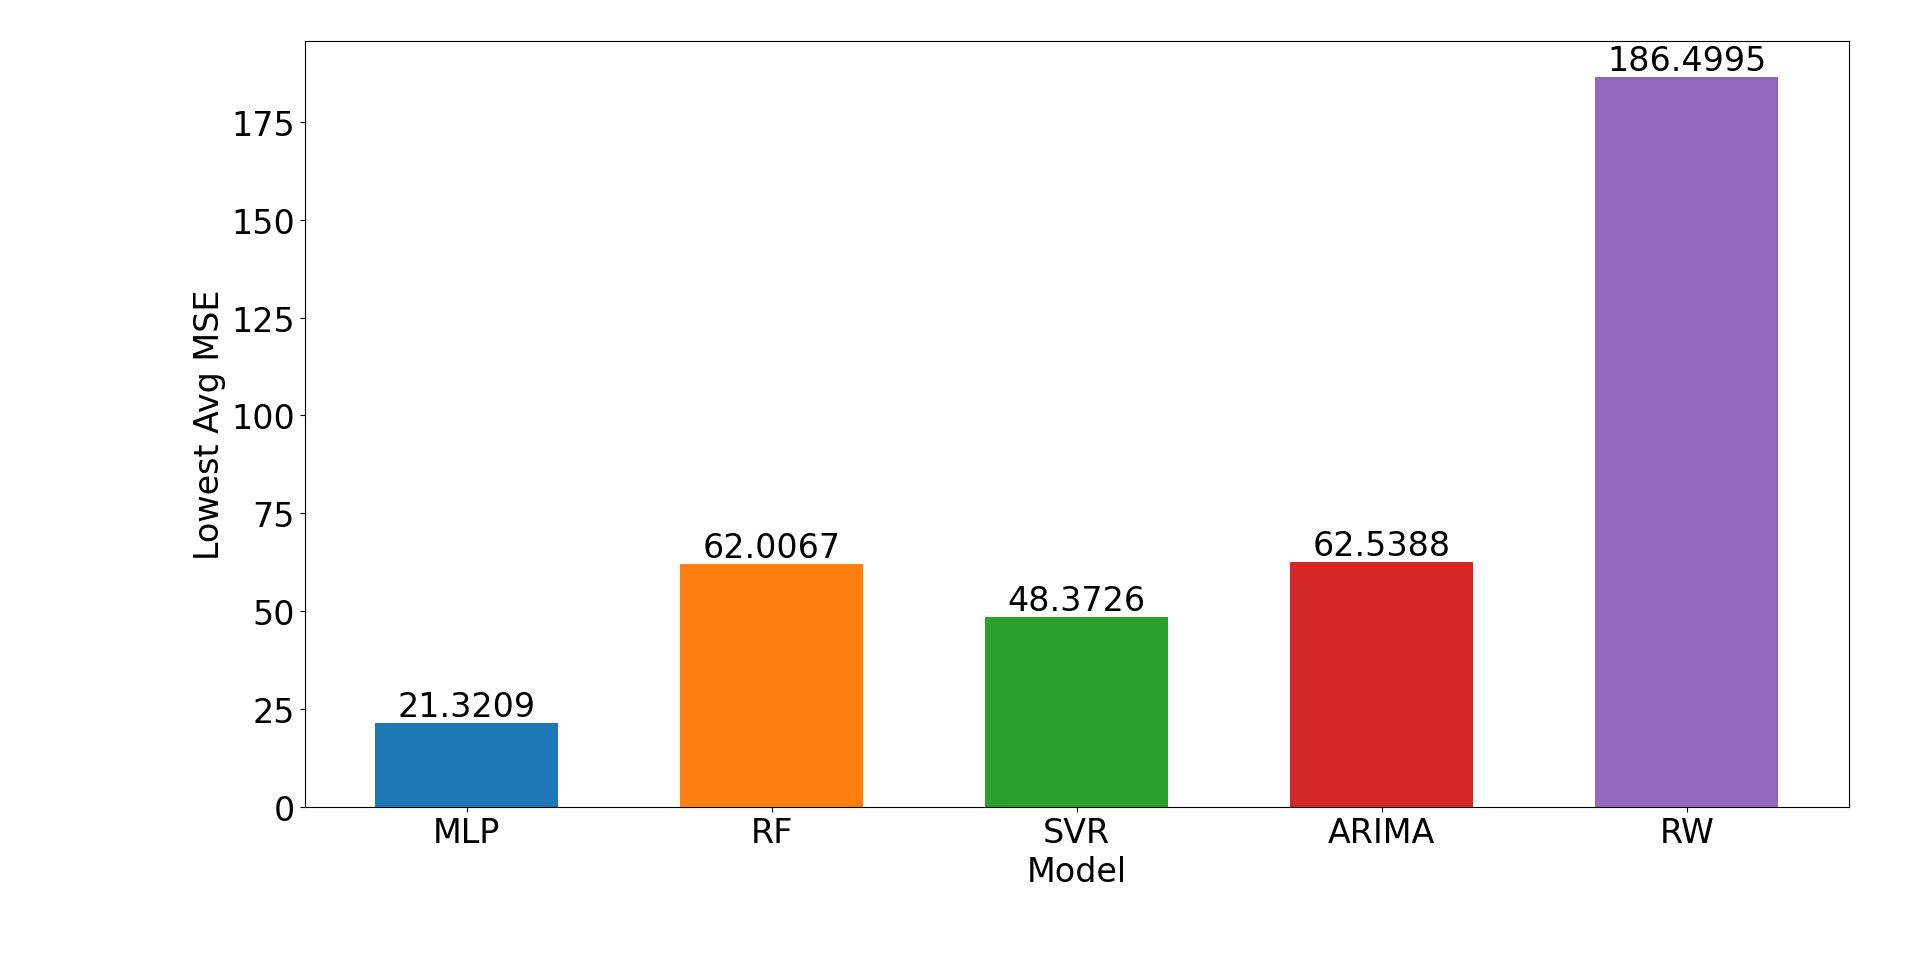
\includegraphics[width=\textwidth]{images/metrics-by-model/mse.png}
    \centering
    \caption{Comparison of the lowest cumulative average of the average \gls{mse} over train and test sets of all offset forecasts for the best dataset preprocessing variant for each model.}
    \label{fig:mse-model-cmp}
\end{figure}

\subsection{Forecasts}\label{Forecasts}

In the next step a cumulative bar chart of the \gls{mse} shown in figure \ref{fig:cumulative-mse} of the forecasts was created to illustrate the relative performance of each model on the basis of it's best dataset preprocessing variant for each offset.

% Bar charts of the offset dependant mse and hitrate of various forecasts

\begin{figure}[h]
    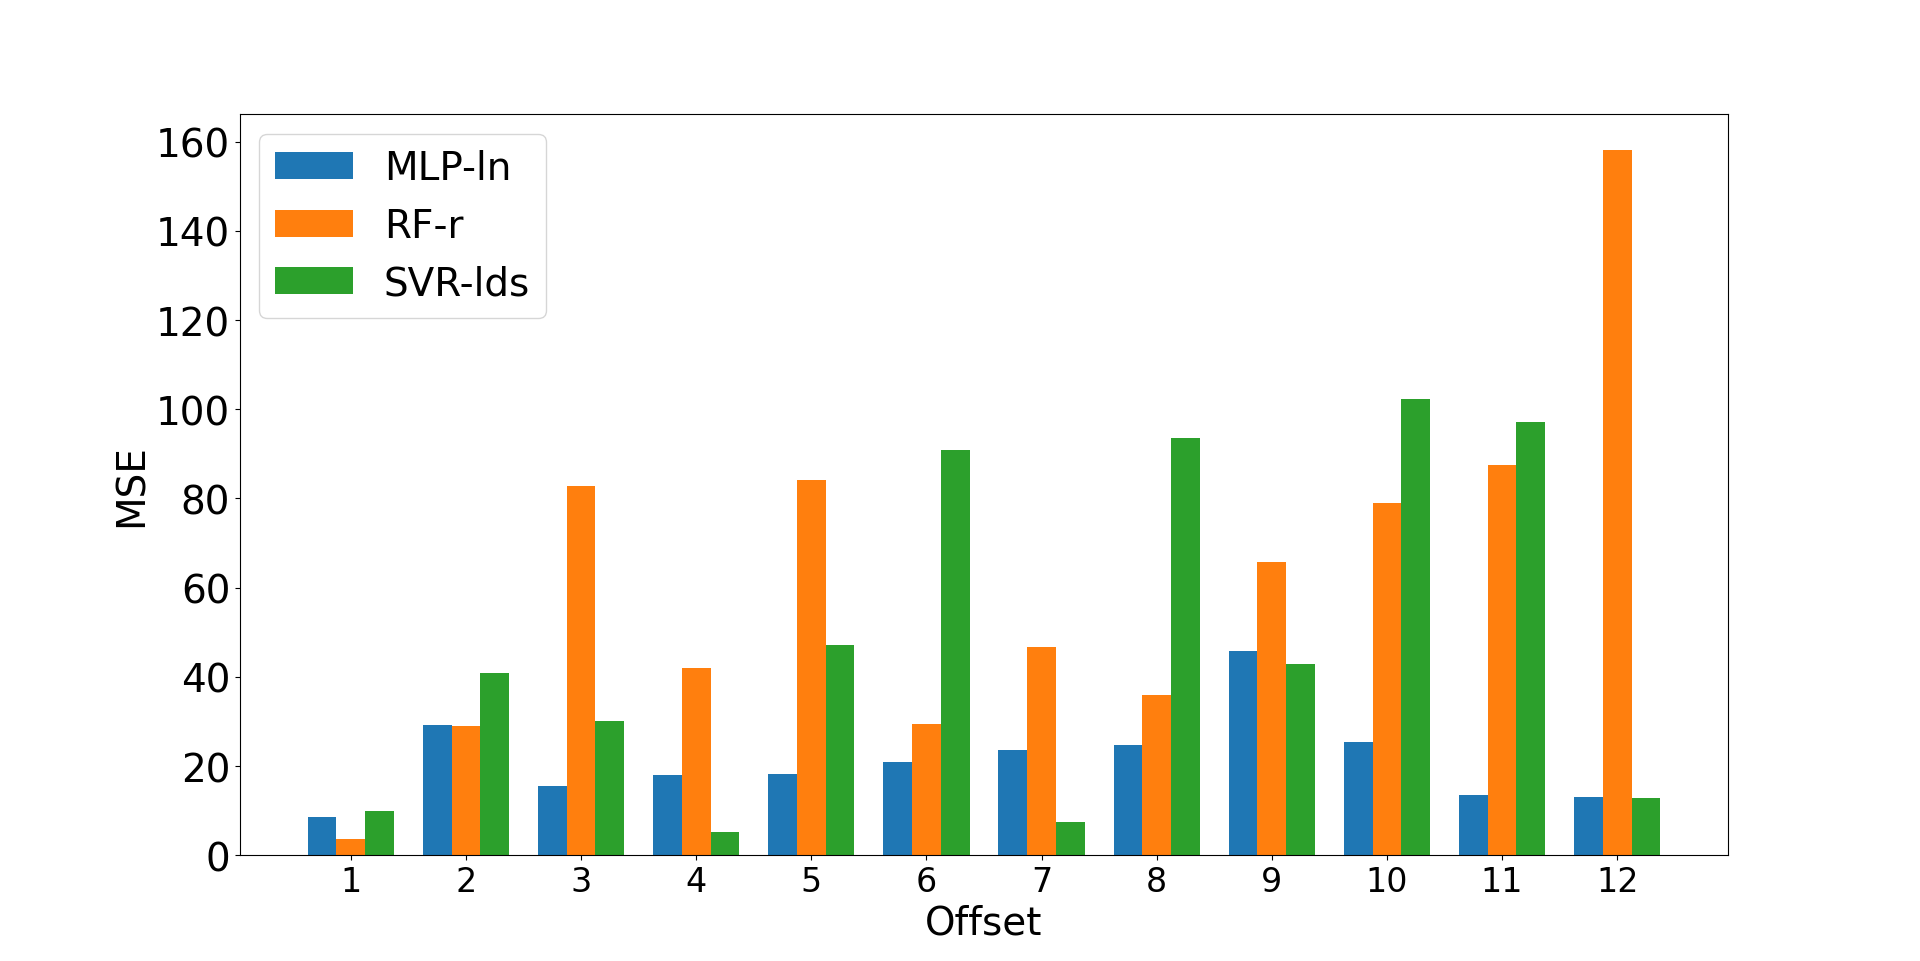
\includegraphics[width=\textwidth]{images/metrics-by-offset/all-mse.png}
    \centering
    \caption{Comparison of the \gls{mse} of the forecasts for the best dataset preprocessing variant for each model for each offset. The sets of processing steps are indicated in shorthand as follows: l - log transformed, d - differenced, n - normalized, s - standardized, r - raw.}
    \label{fig:cumulative-mse}
\end{figure}

Additionally as can be seen below in figures from \ref{fig:forecast-cmp-1} to \ref{fig:forecast-cmp-12} the reverse transformed forecasts for each model for the USD currency were plotted for each offset.

\begin{figure}[h]
    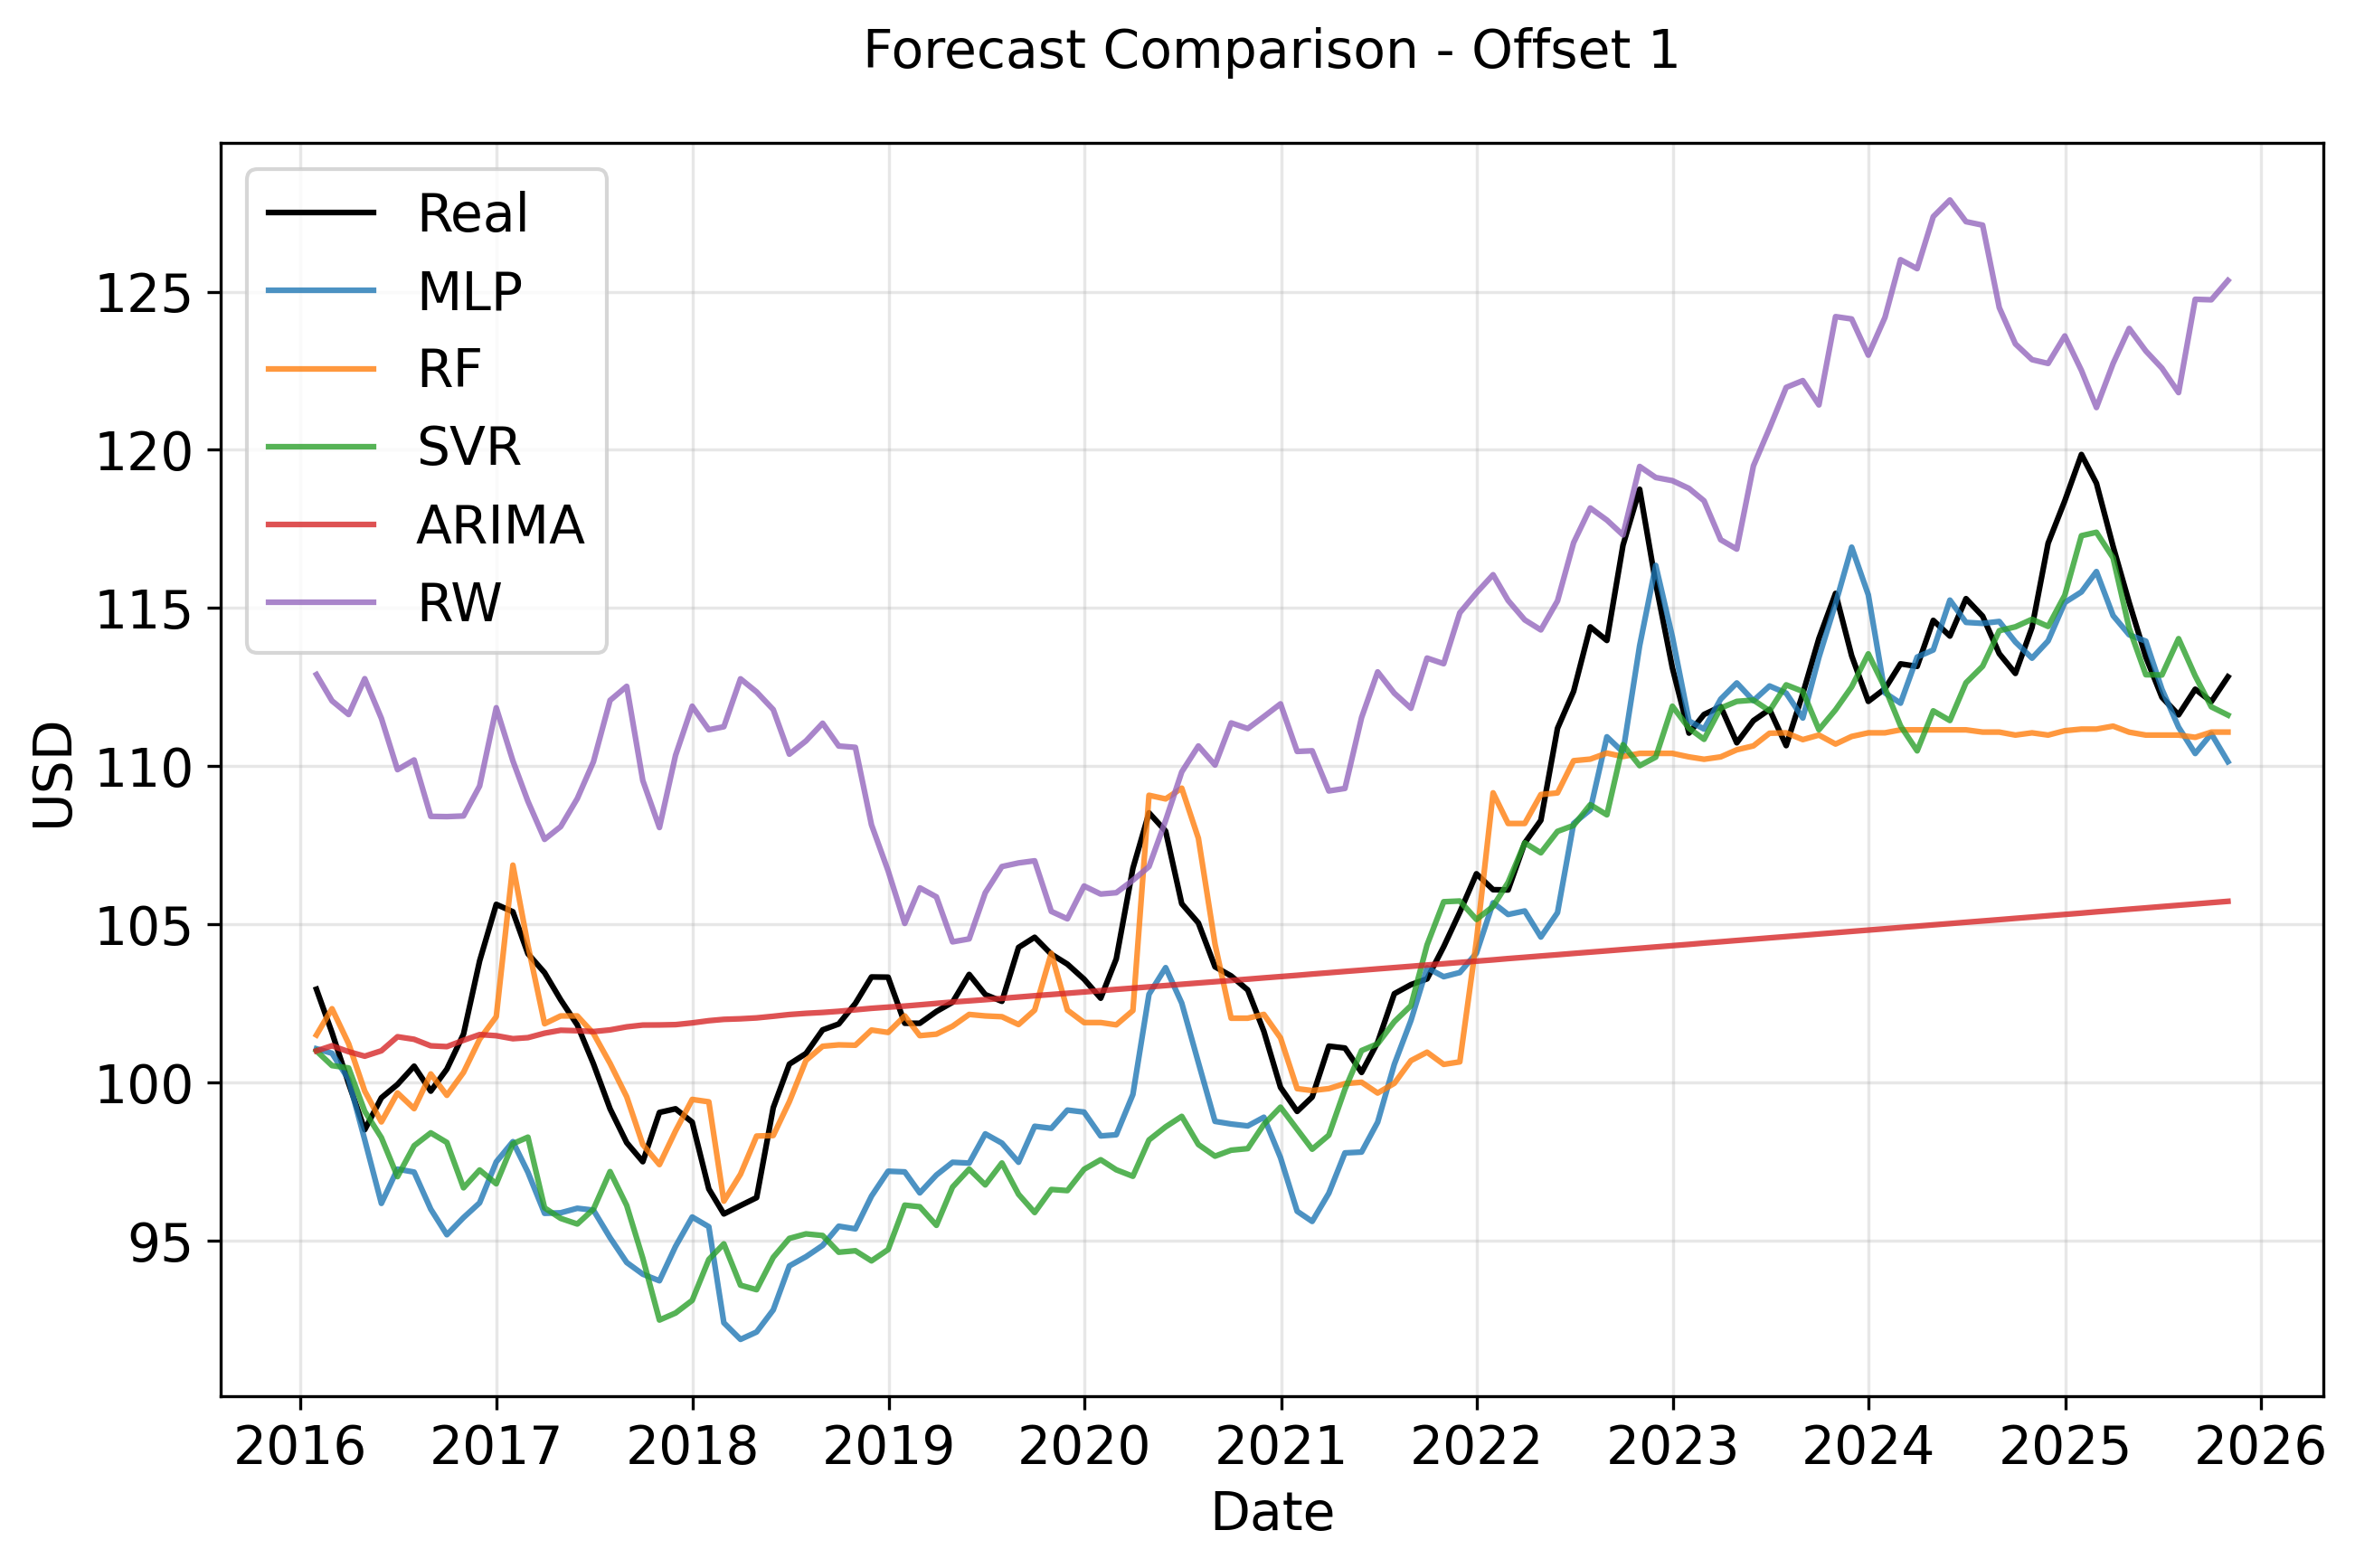
\includegraphics[width=\textwidth]{images/forecast-comparison/mse/1.png}
    \centering
    \caption{The best \gls{mse} forecasts per selected dataset per model for an offset of 1 month.}
    \label{fig:forecast-cmp-1}
\end{figure}

\begin{figure}[h]
    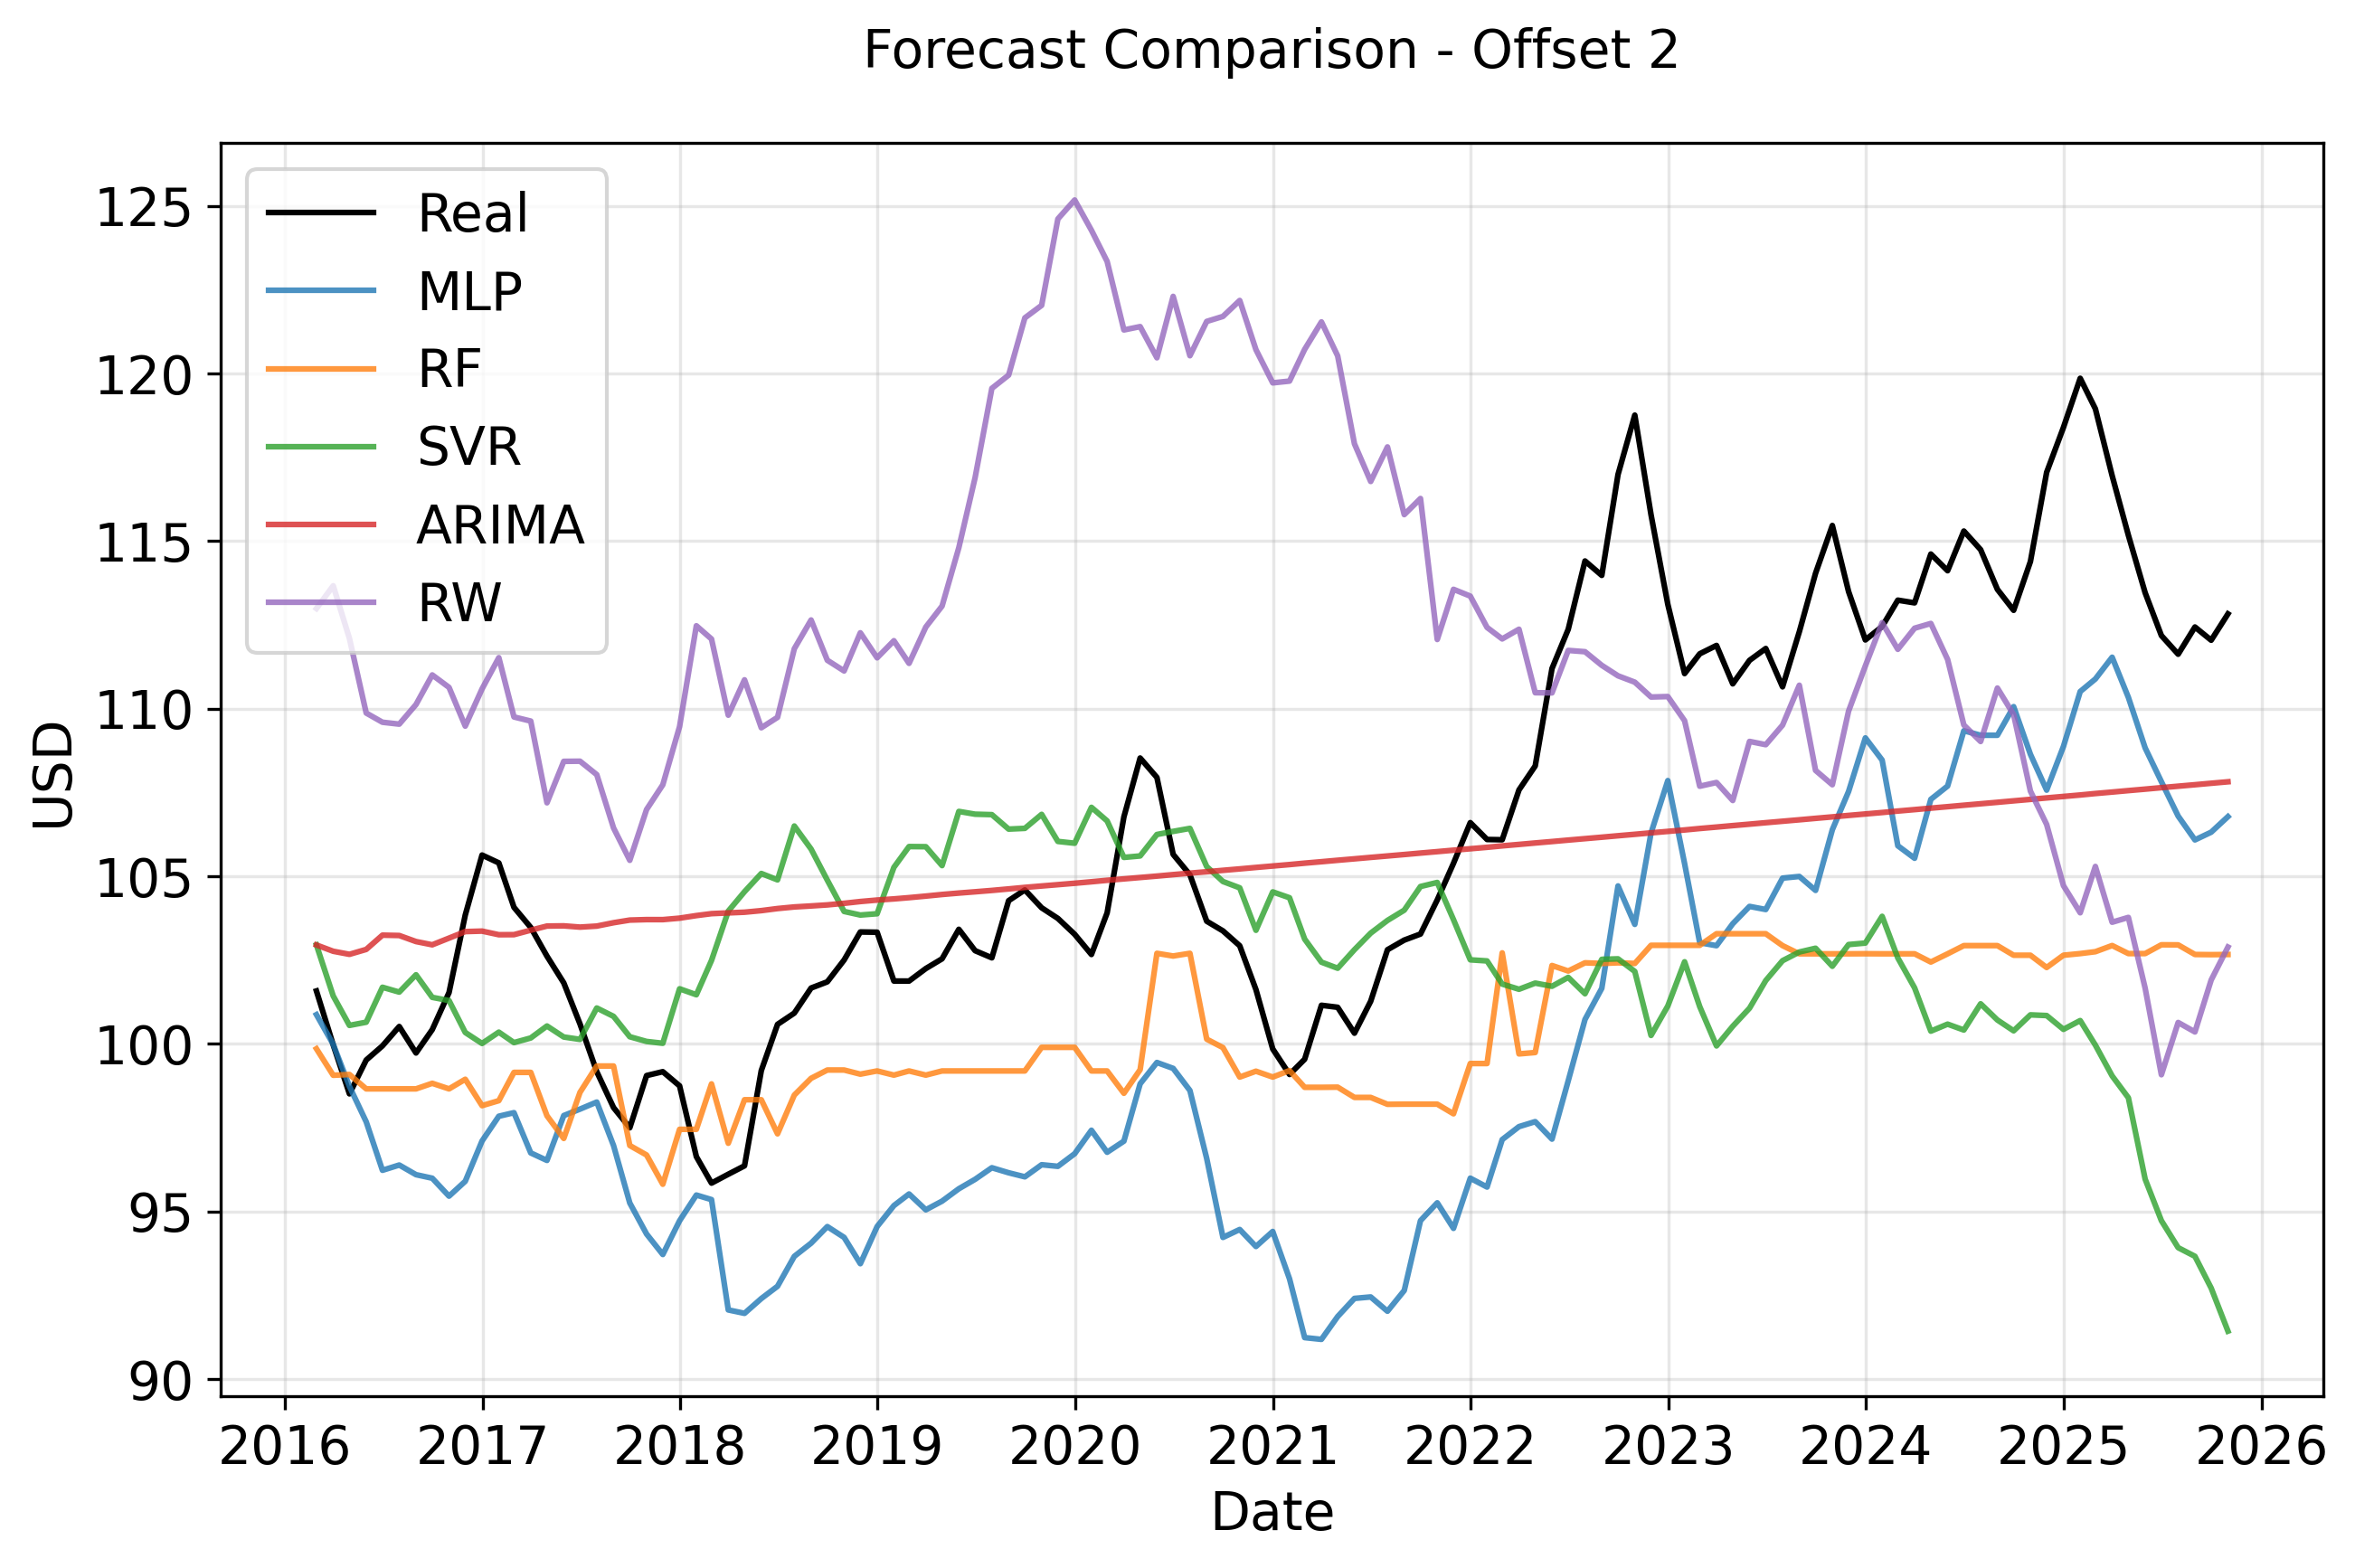
\includegraphics[width=\textwidth]{images/forecast-comparison/mse/2.png}
    \centering
    \caption{The best \gls{mse} forecasts per selected dataset per model for an offset of 2 months.}
    \label{fig:forecast-cmp-2}
\end{figure}

\begin{figure}[h]
    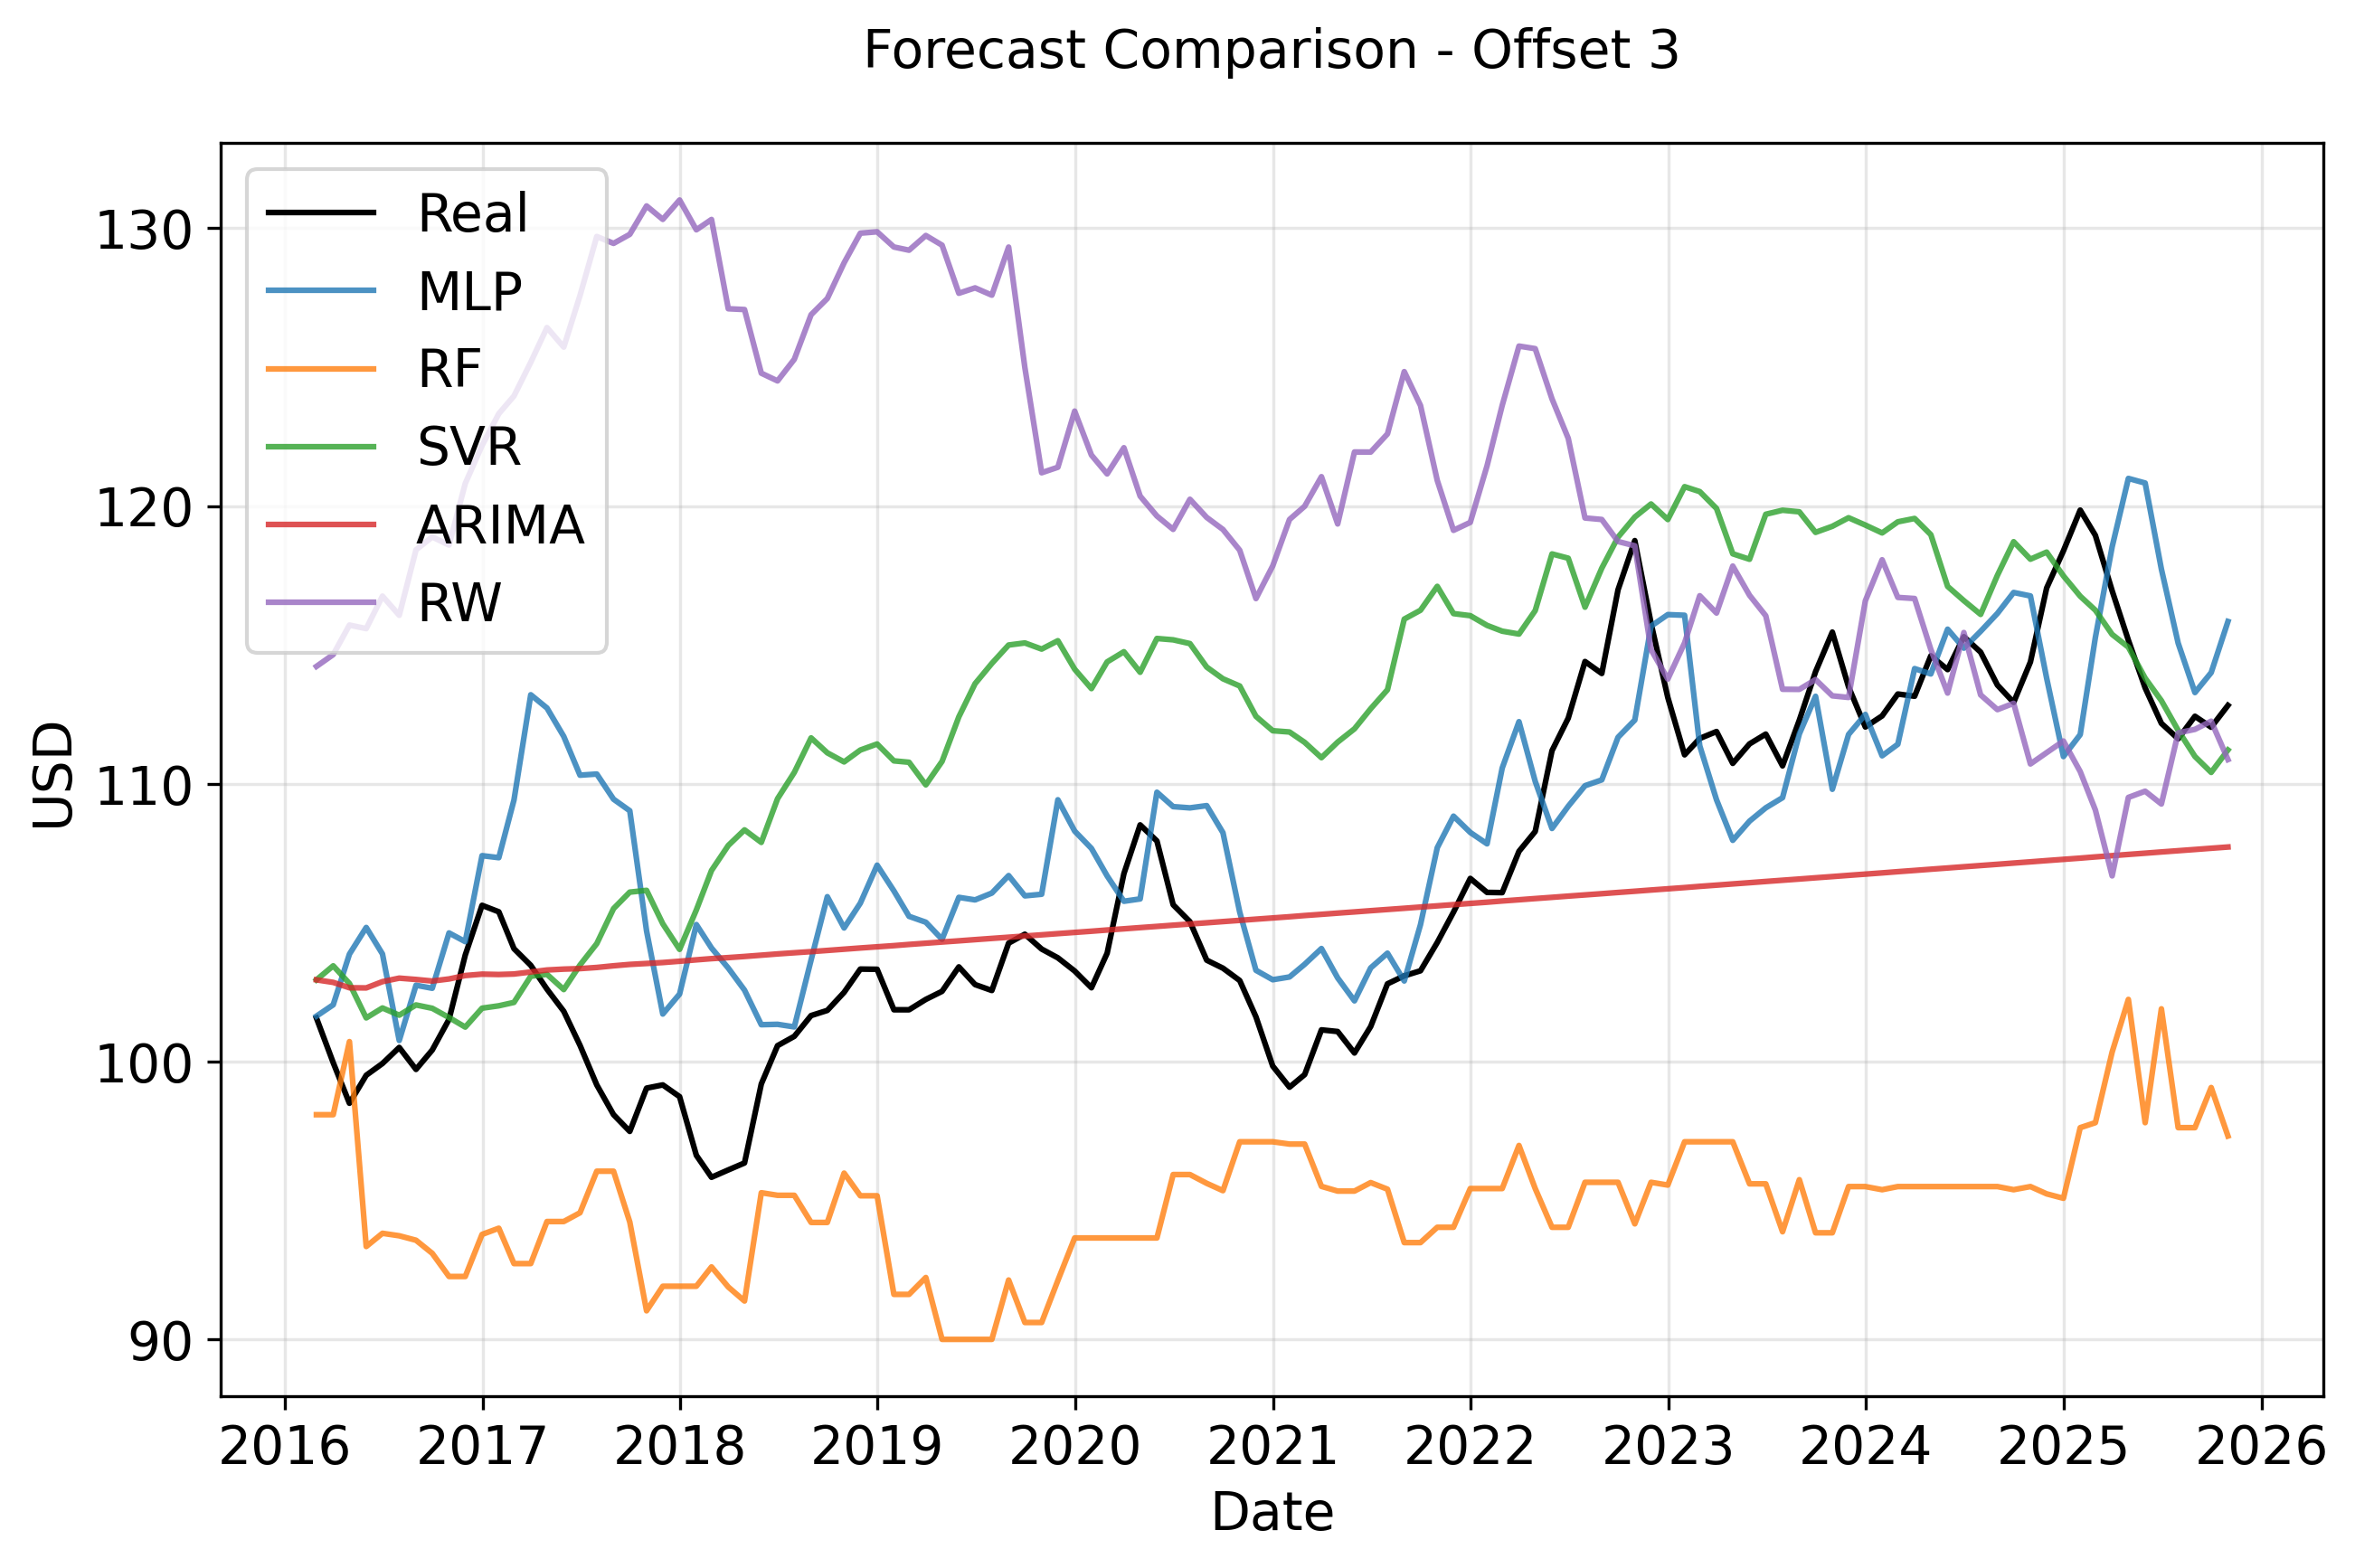
\includegraphics[width=\textwidth]{images/forecast-comparison/mse/3.png}
    \centering
    \caption{The best \gls{mse} forecasts per selected dataset per model for an offset of 3 months.}
    \label{fig:forecast-cmp-3}
\end{figure}

\begin{figure}[h]
    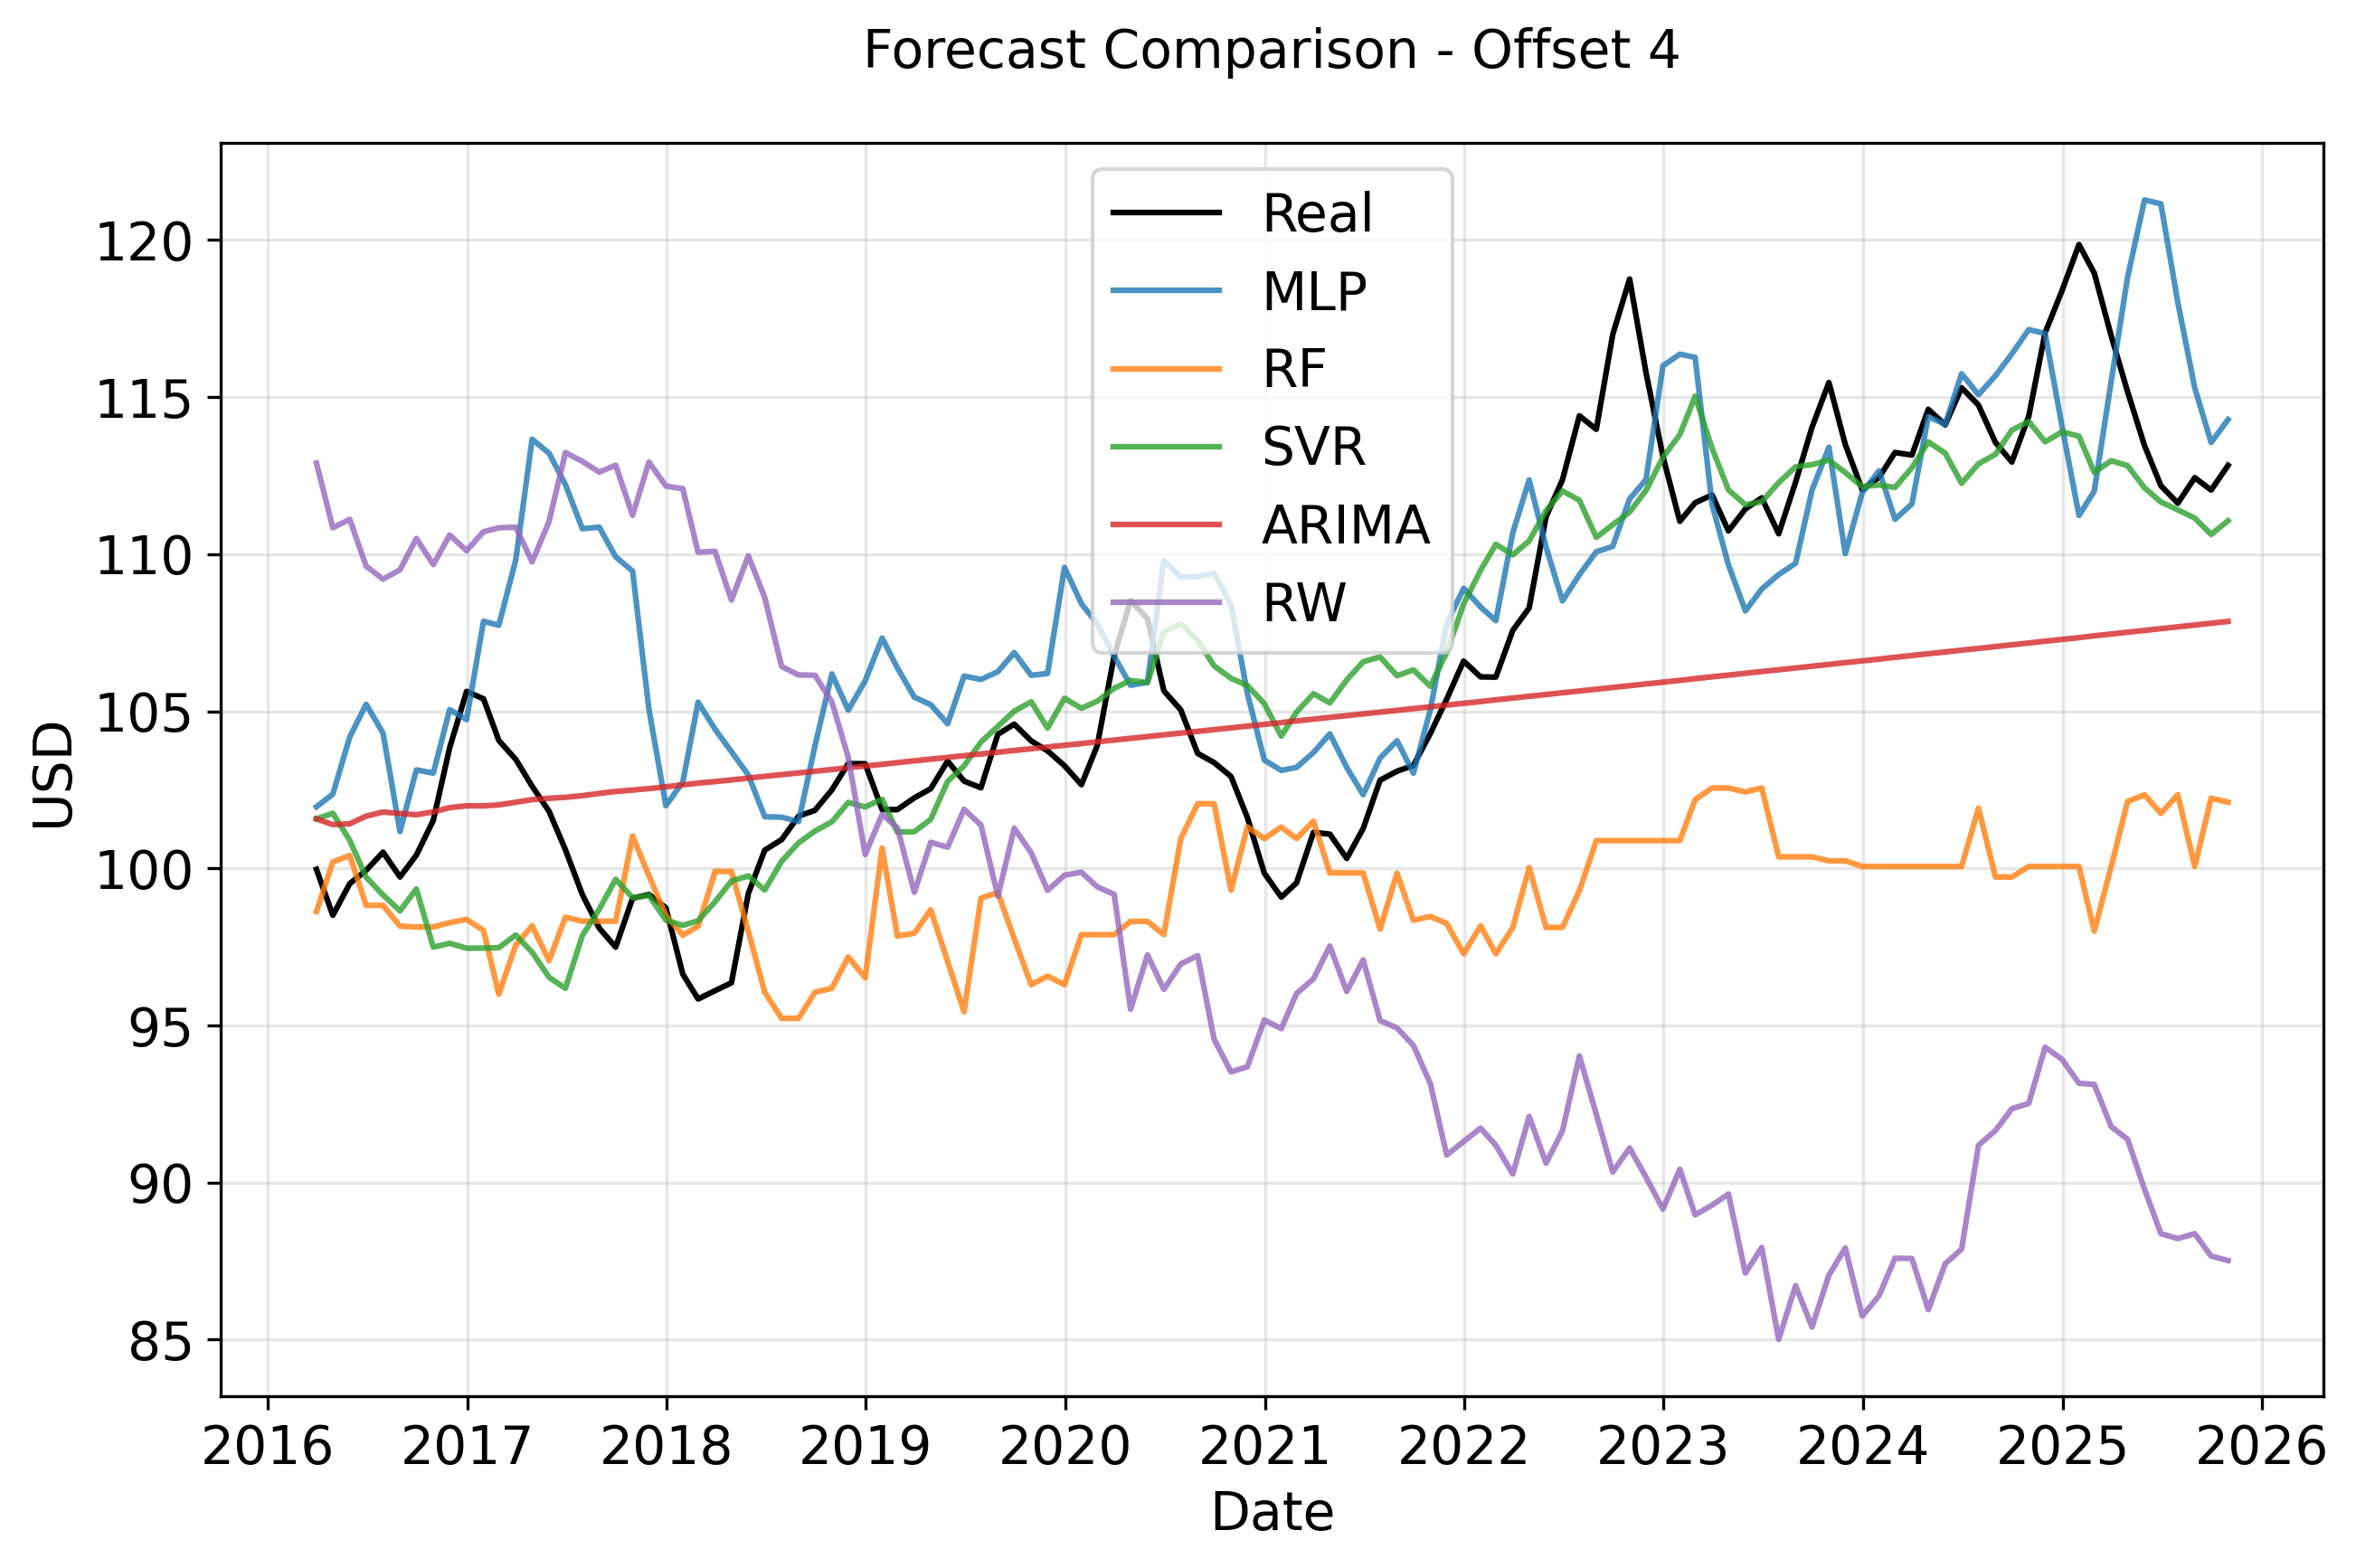
\includegraphics[width=\textwidth]{images/forecast-comparison/mse/4.png}
    \centering
    \caption{The best \gls{mse} forecasts per selected dataset per model for an offset of 4 months.}
    \label{fig:forecast-cmp-4}
\end{figure}

\begin{figure}[h]
    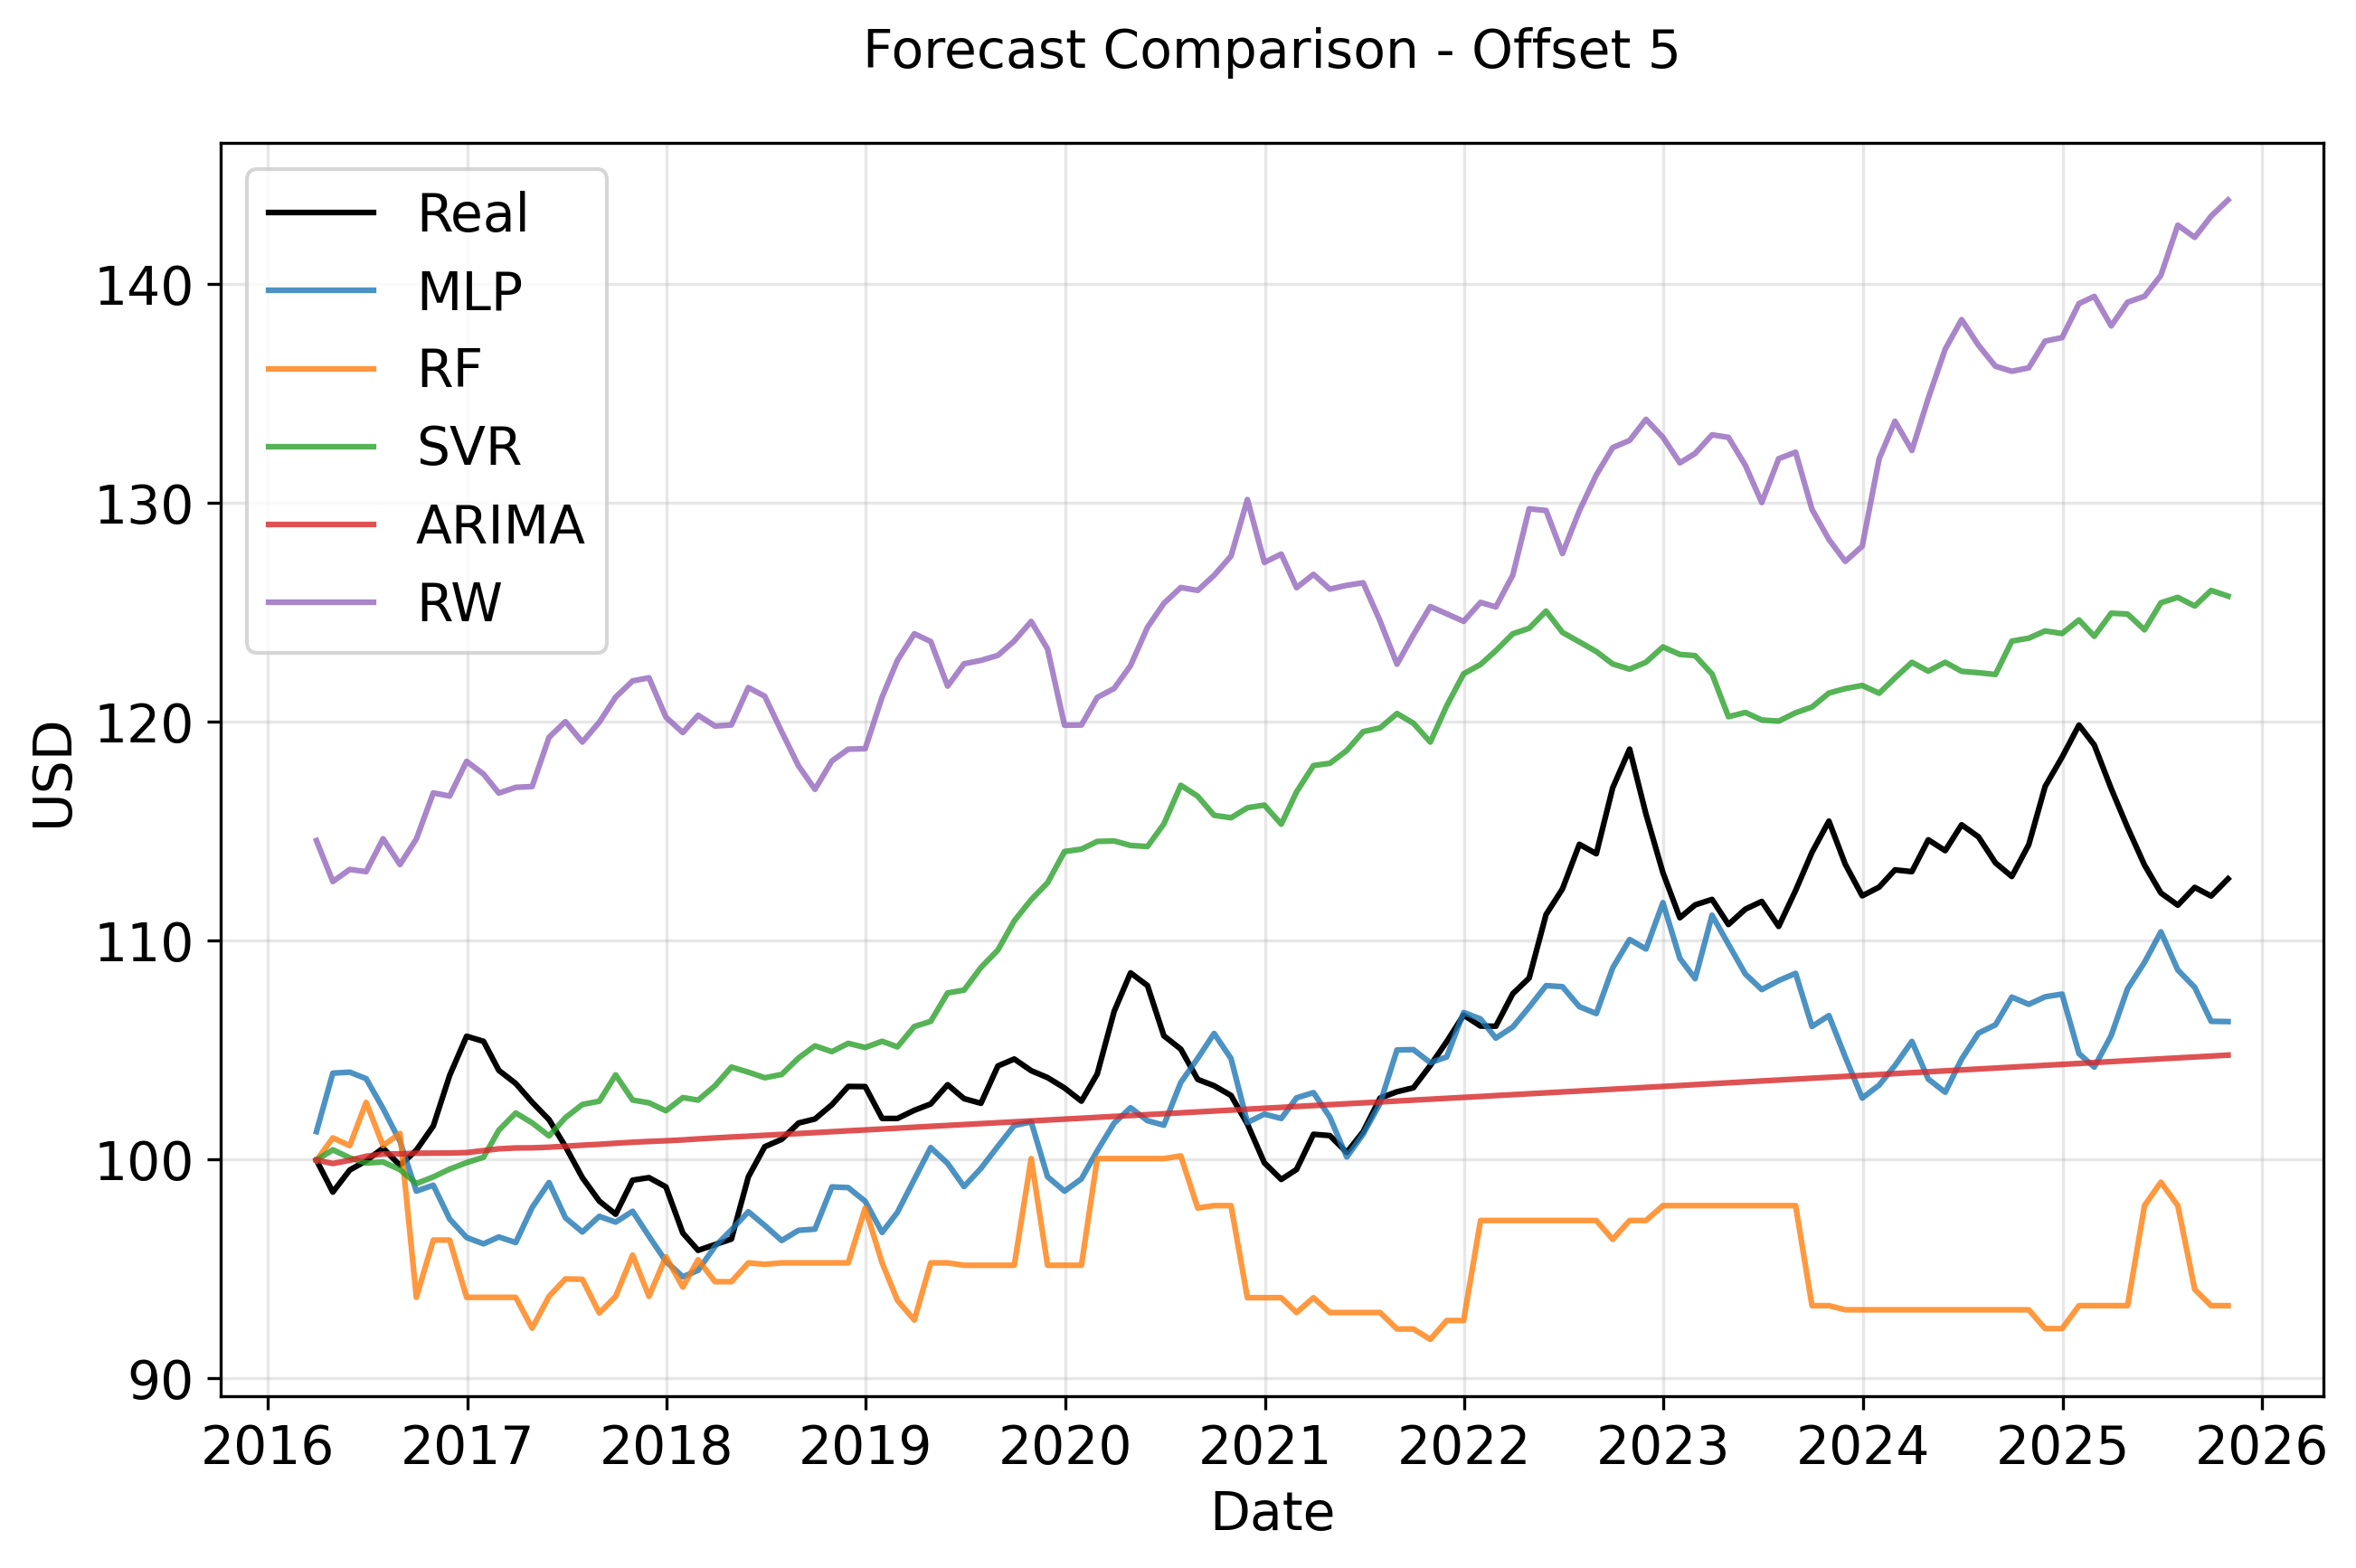
\includegraphics[width=\textwidth]{images/forecast-comparison/mse/5.png}
    \centering
    \caption{The best \gls{mse} forecasts per selected dataset per model for an offset of 5 months.}
    \label{fig:forecast-cmp-5}
\end{figure}

\begin{figure}[h]
    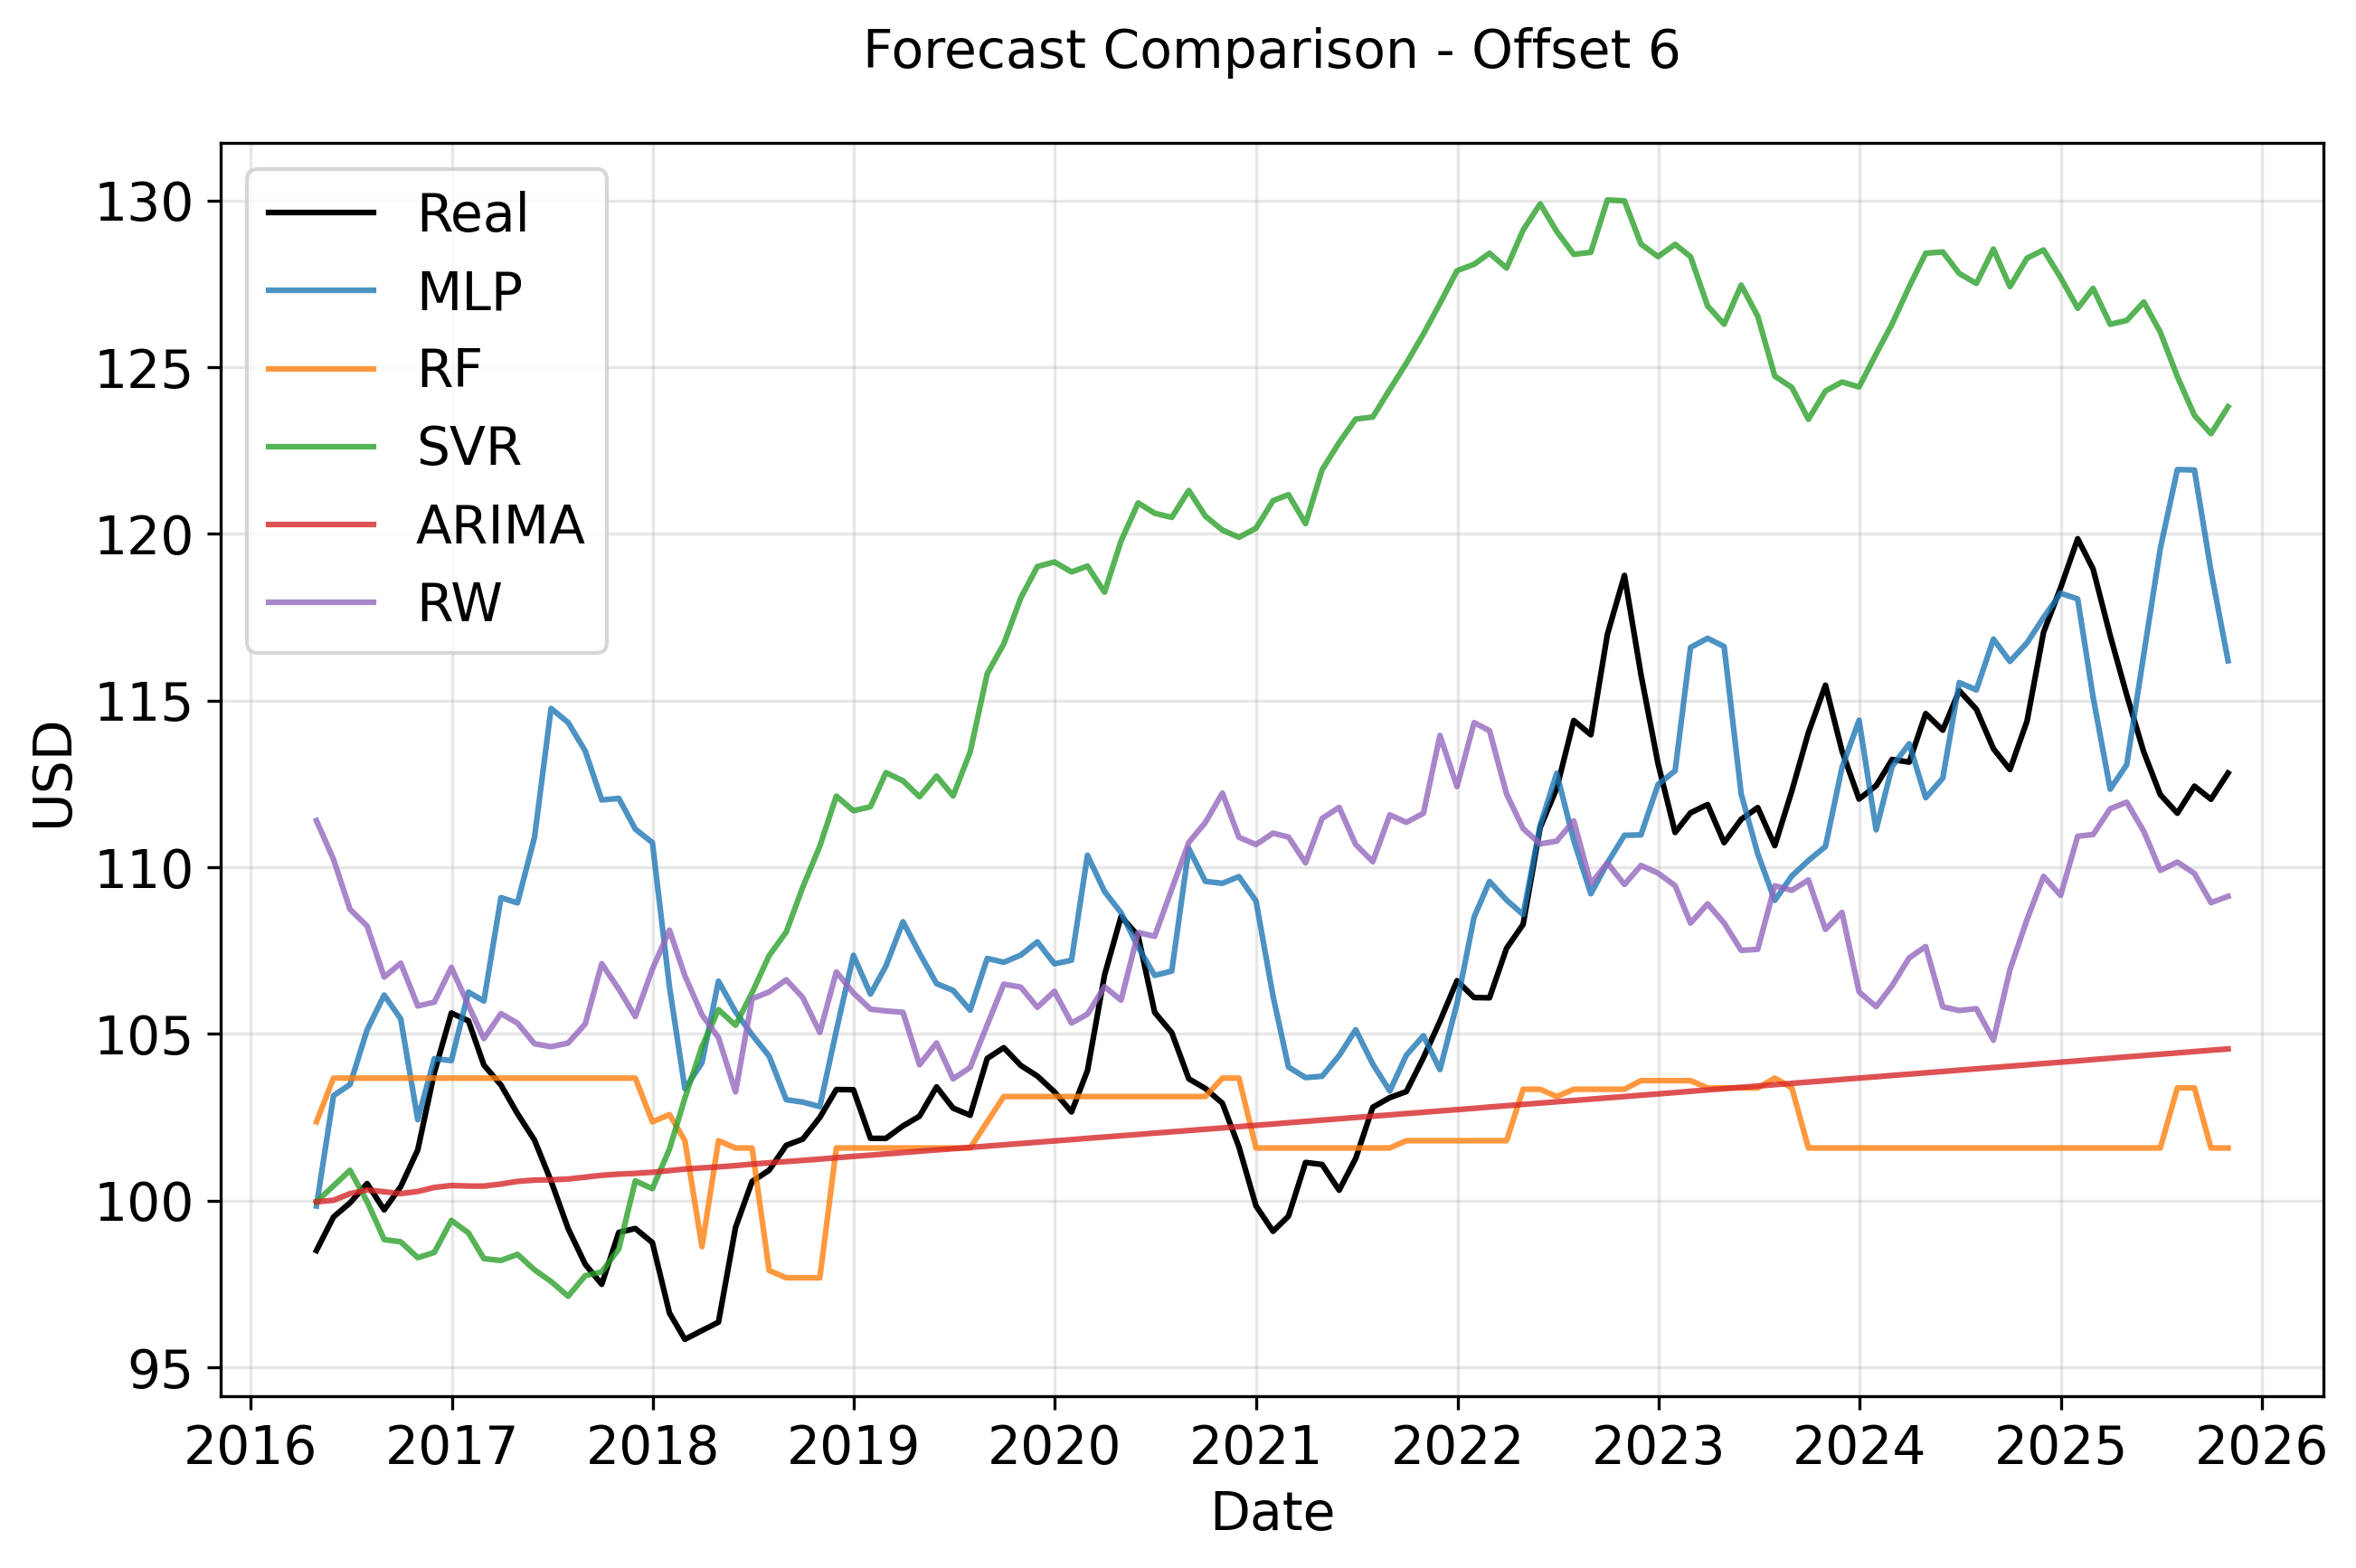
\includegraphics[width=\textwidth]{images/forecast-comparison/mse/6.png}
    \centering
    \caption{The best \gls{mse} forecasts per selected dataset per model for an offset of 6 months.}
    \label{fig:forecast-cmp-6}
\end{figure}

\begin{figure}[h]
    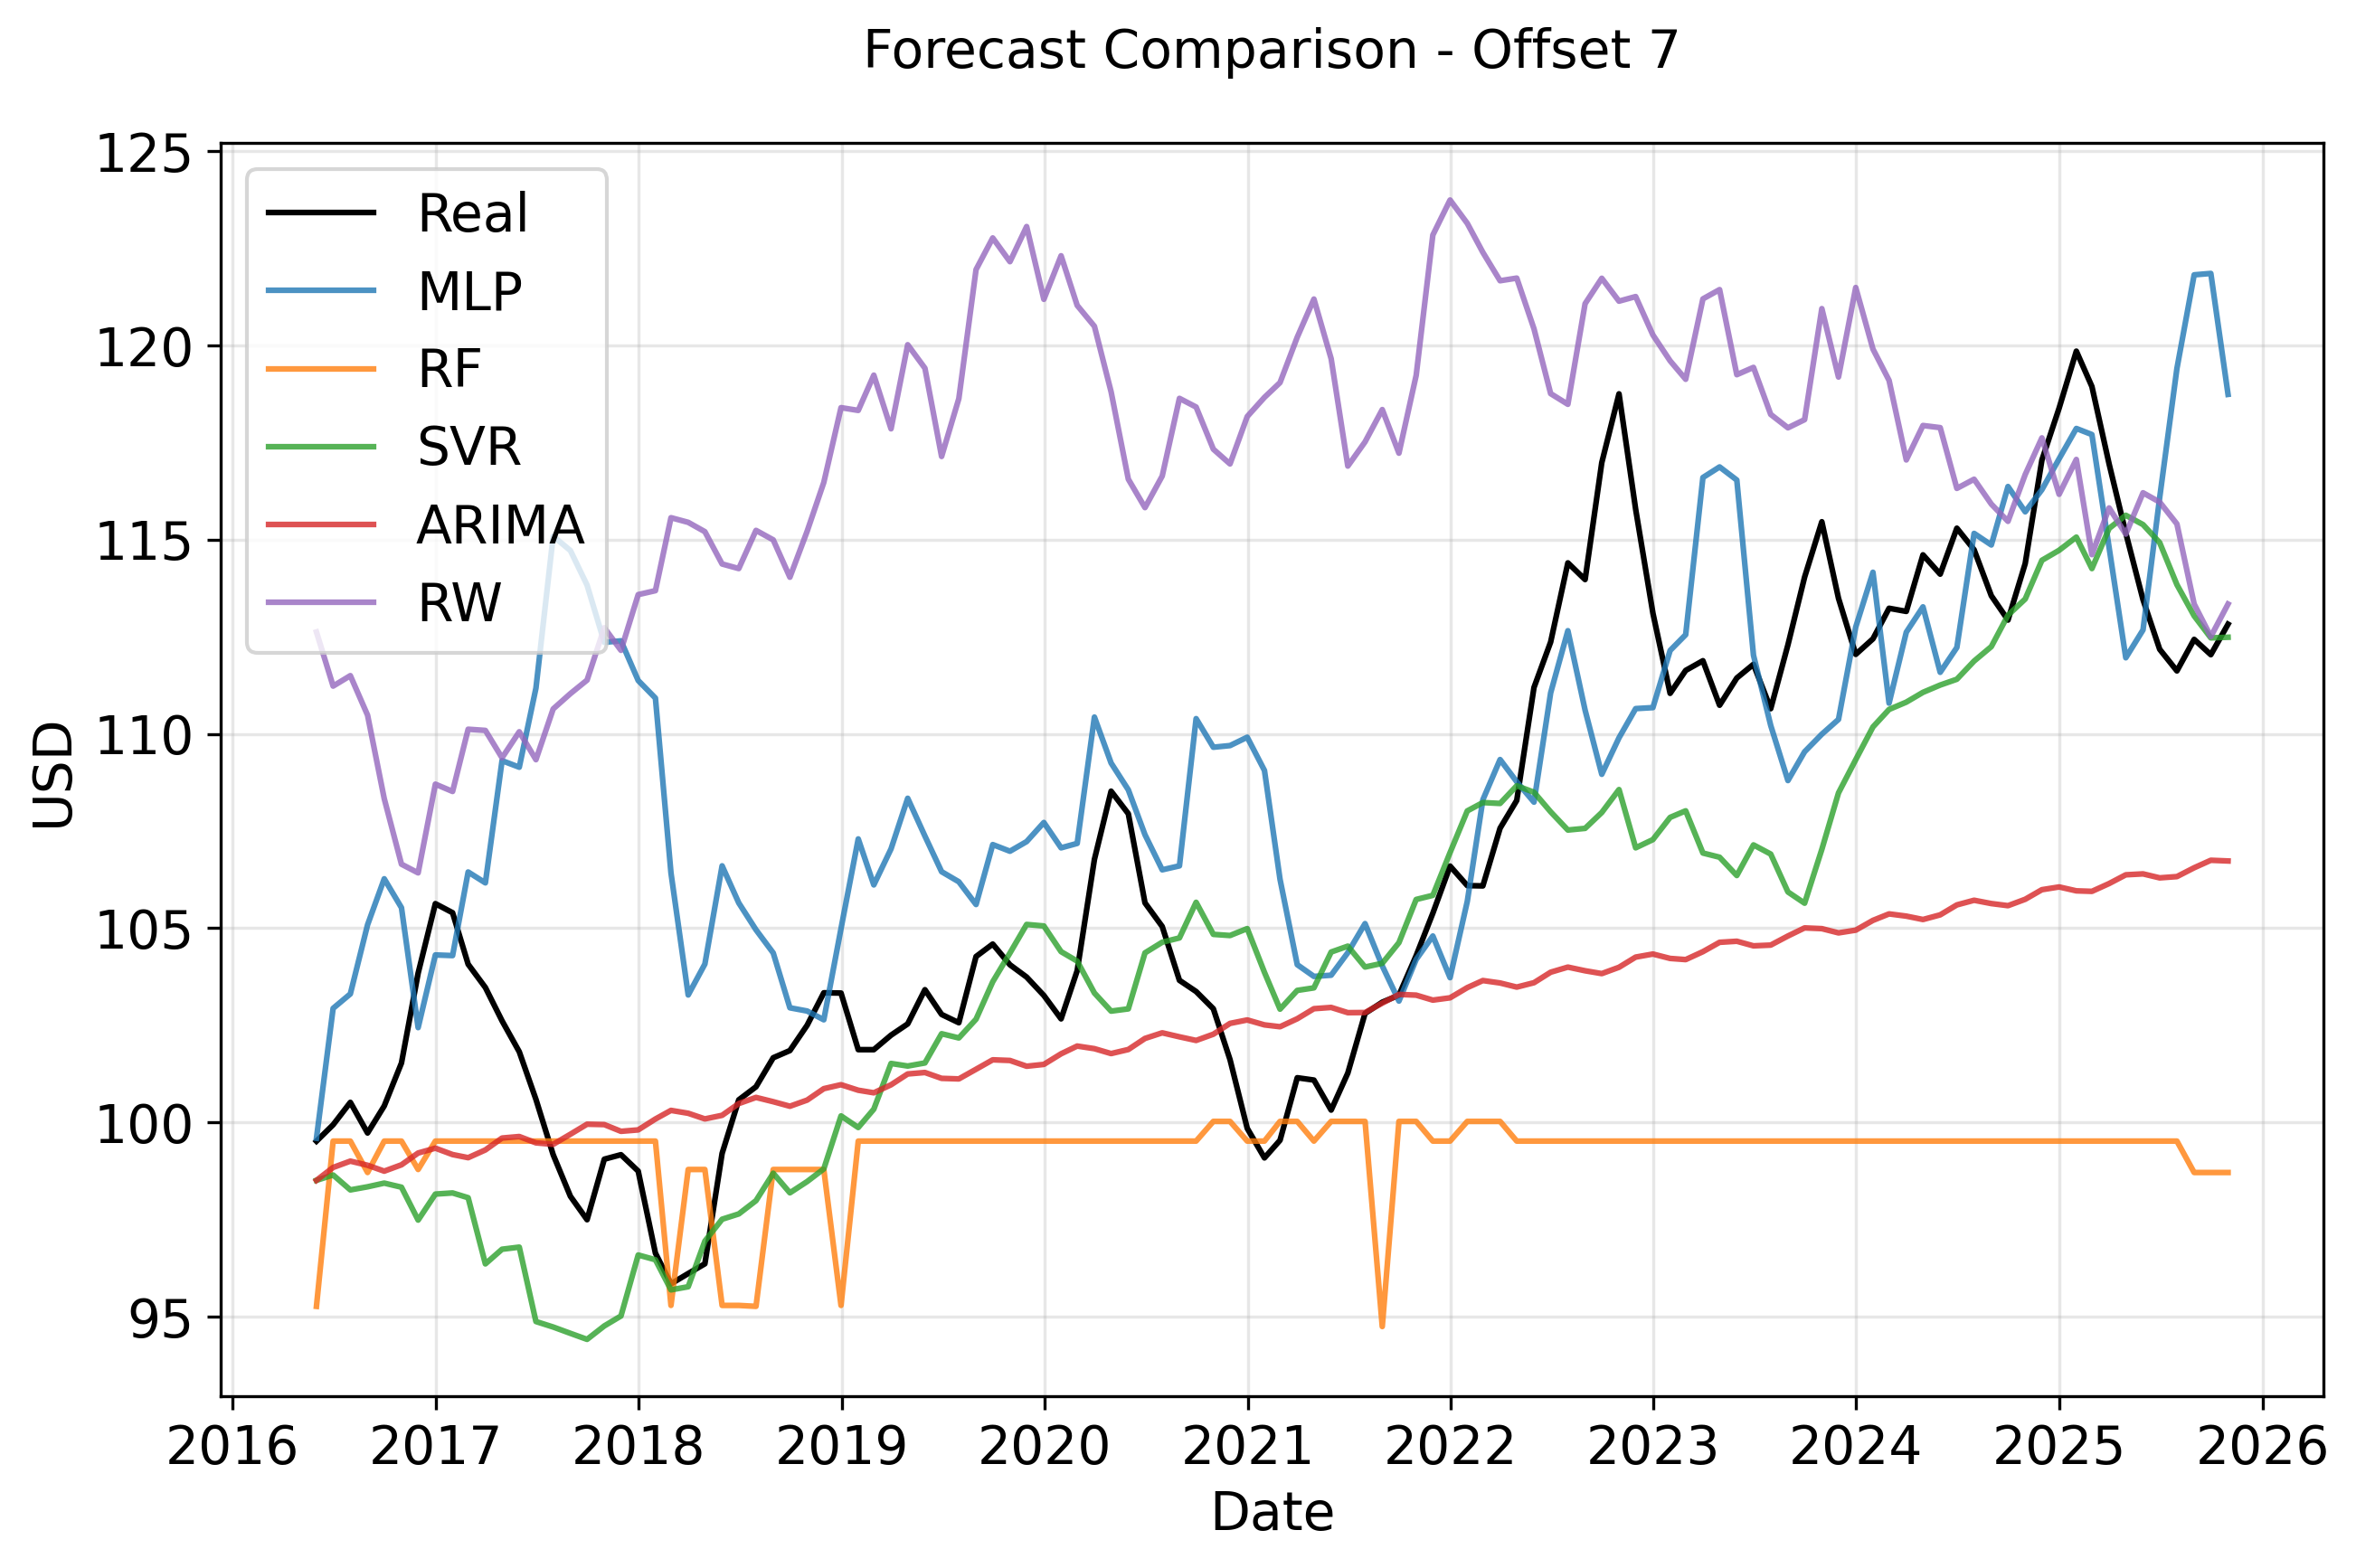
\includegraphics[width=\textwidth]{images/forecast-comparison/mse/7.png}
    \centering
    \caption{The best \gls{mse} forecasts per selected dataset per model for an offset of 7 months.}
    \label{fig:forecast-cmp-7}
\end{figure}

\begin{figure}[h]
    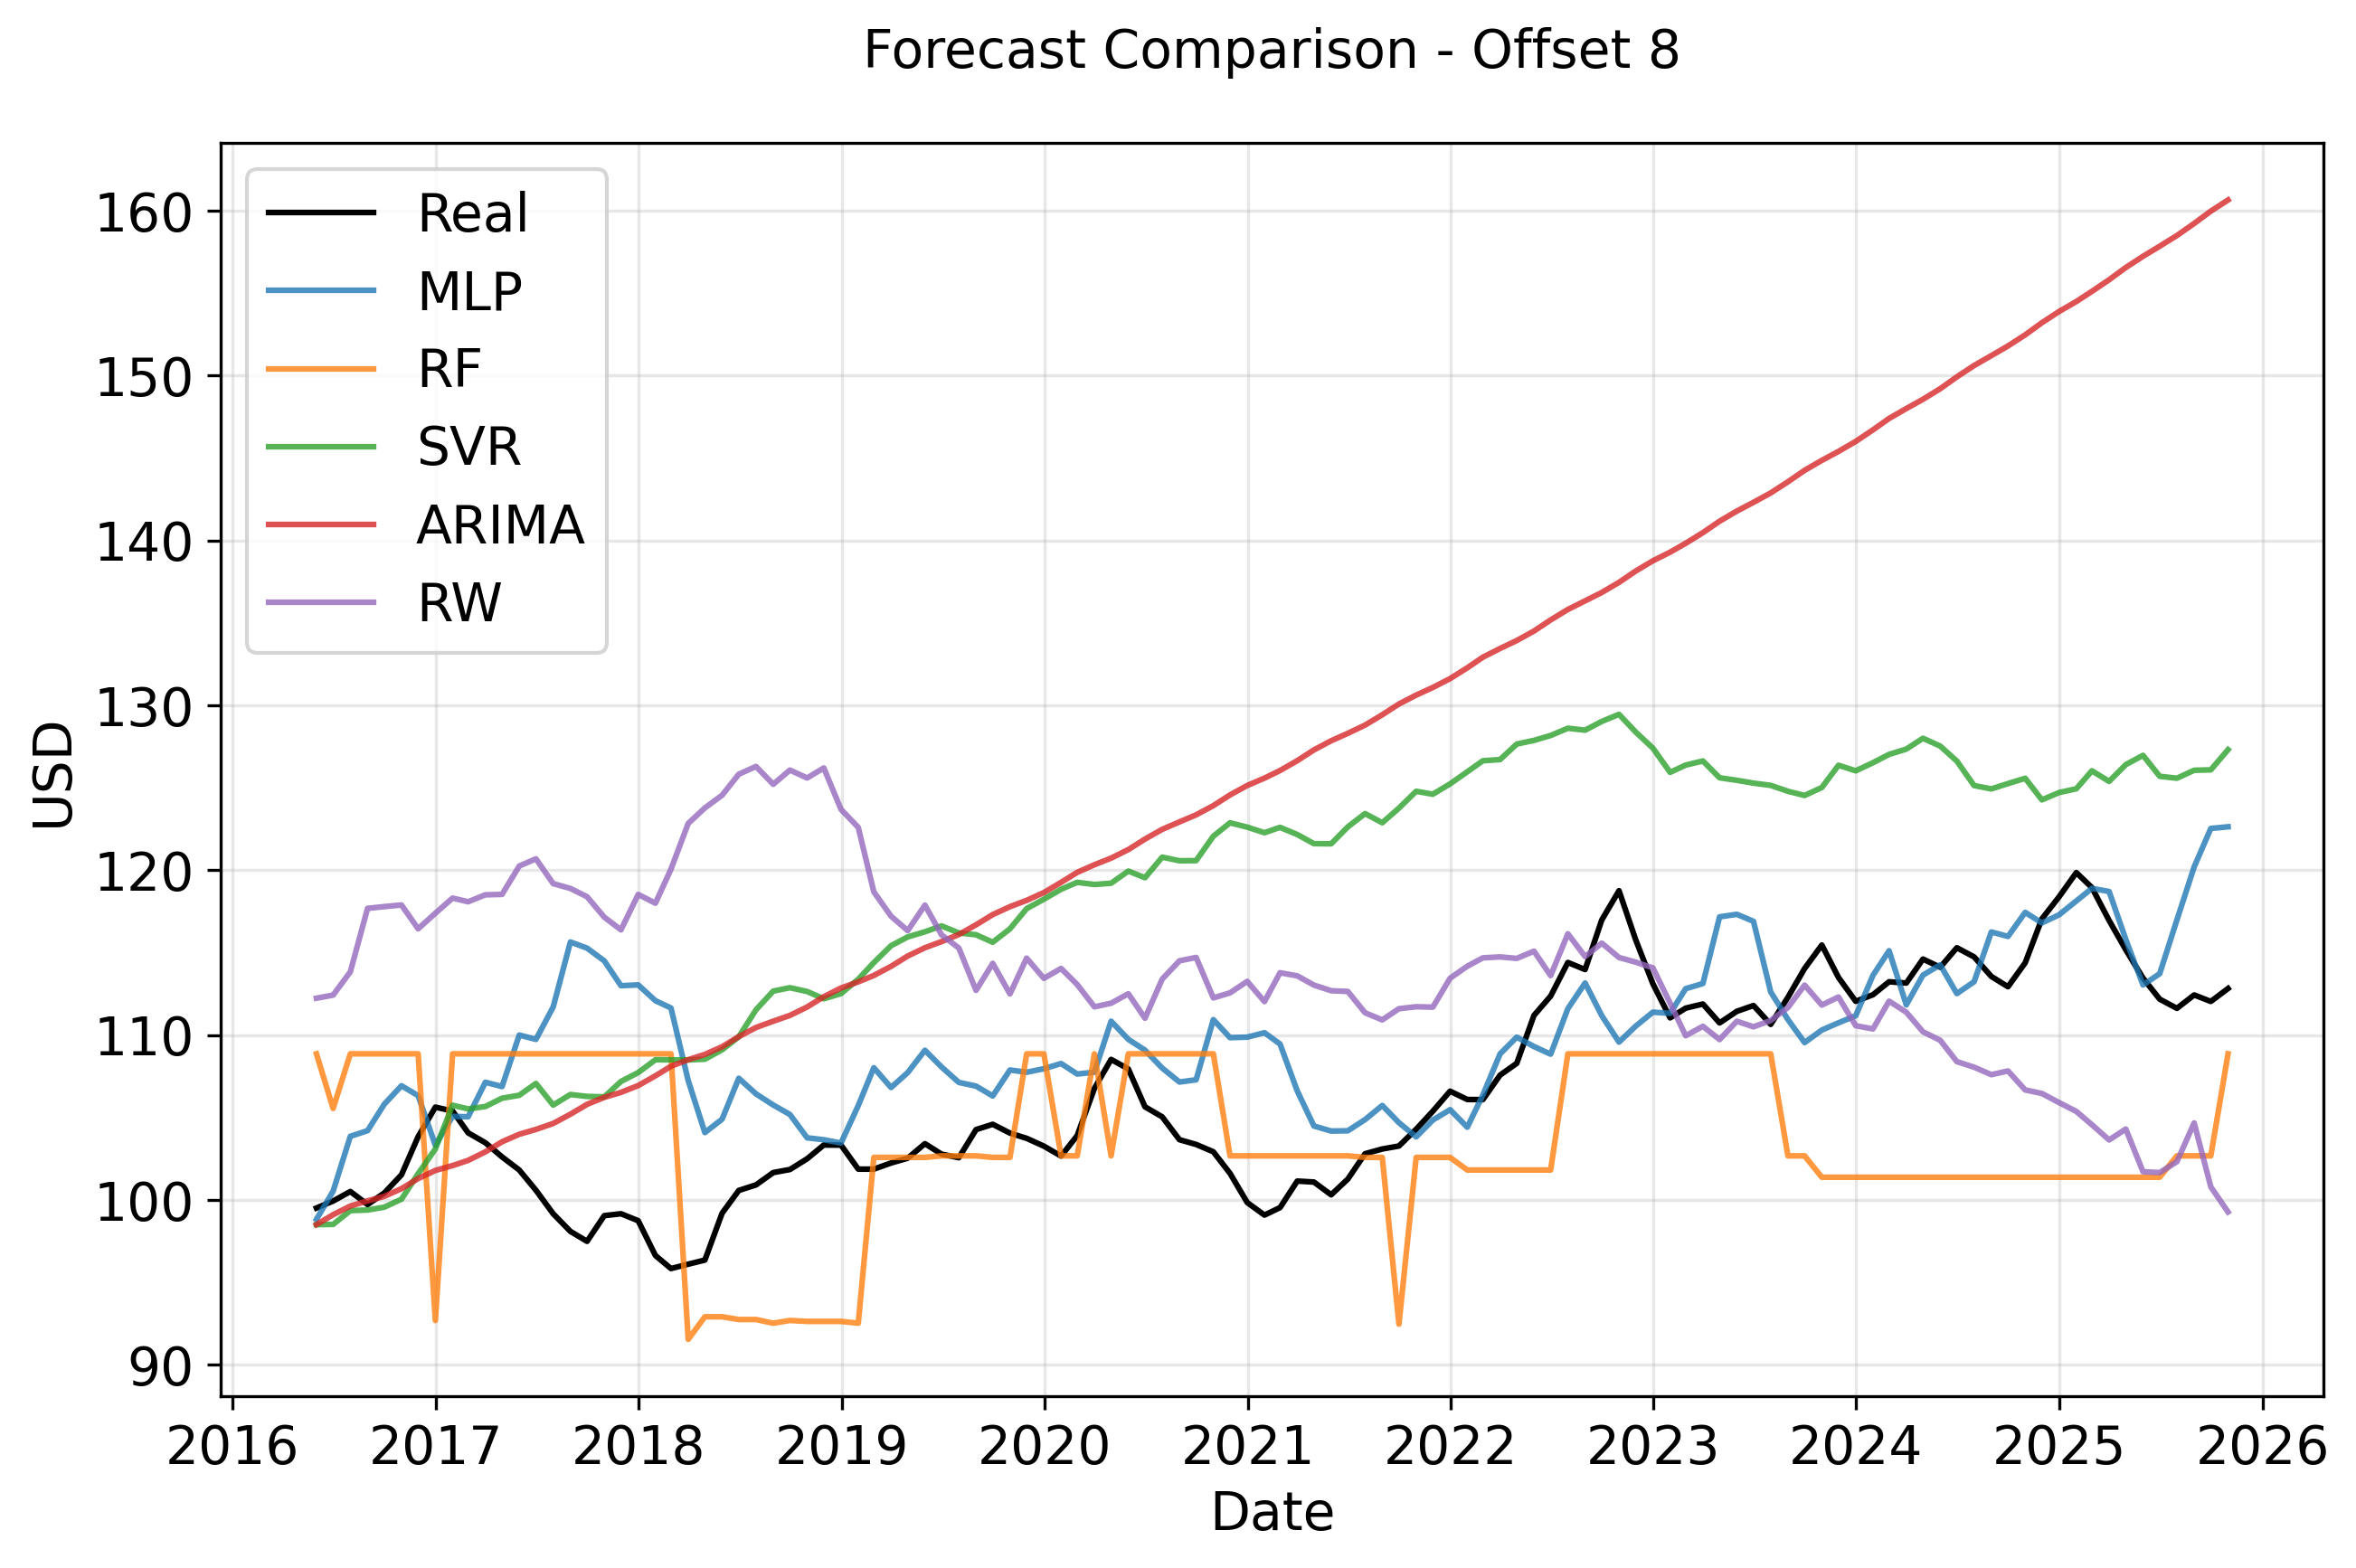
\includegraphics[width=\textwidth]{images/forecast-comparison/mse/8.png}
    \centering
    \caption{The best \gls{mse} forecasts per selected dataset per model for an offset of 8 months.}
    \label{fig:forecast-cmp-8}
\end{figure}

\begin{figure}[h]
    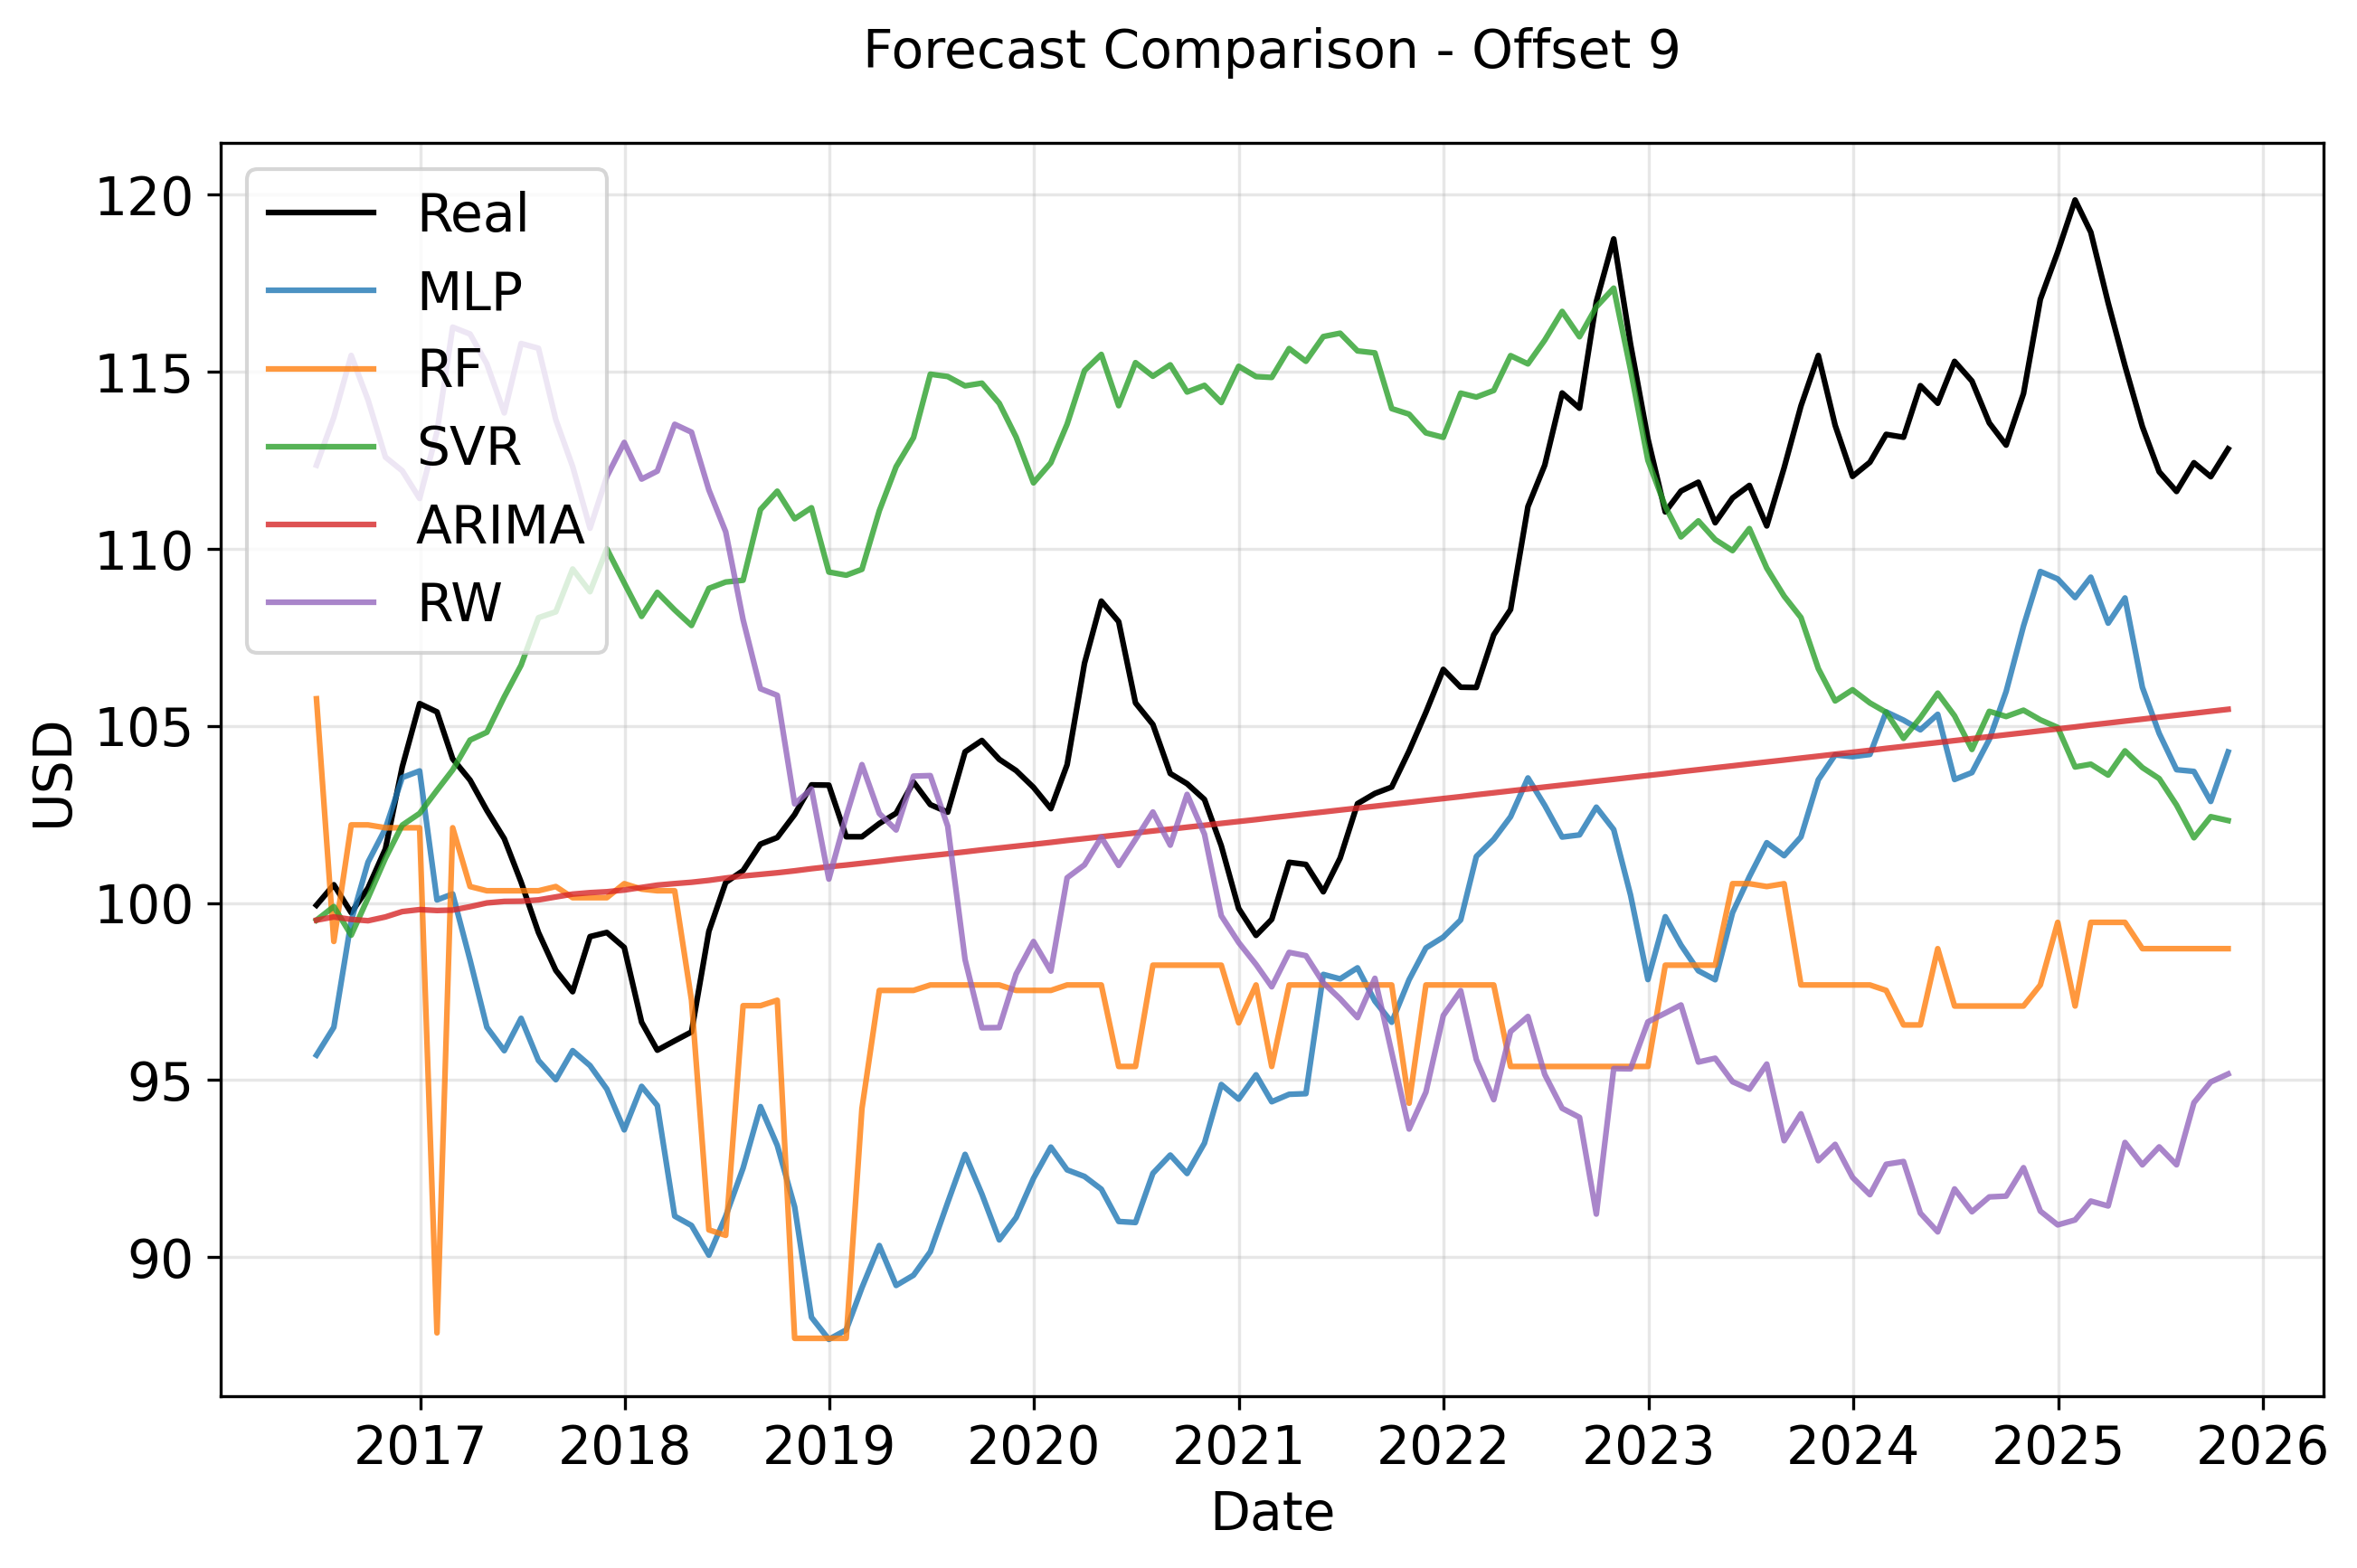
\includegraphics[width=\textwidth]{images/forecast-comparison/mse/9.png}
    \centering
    \caption{The best \gls{mse} forecasts per selected dataset per model for an offset of 9 months.}
    \label{fig:forecast-cmp-9}
\end{figure}

\begin{figure}[h]
    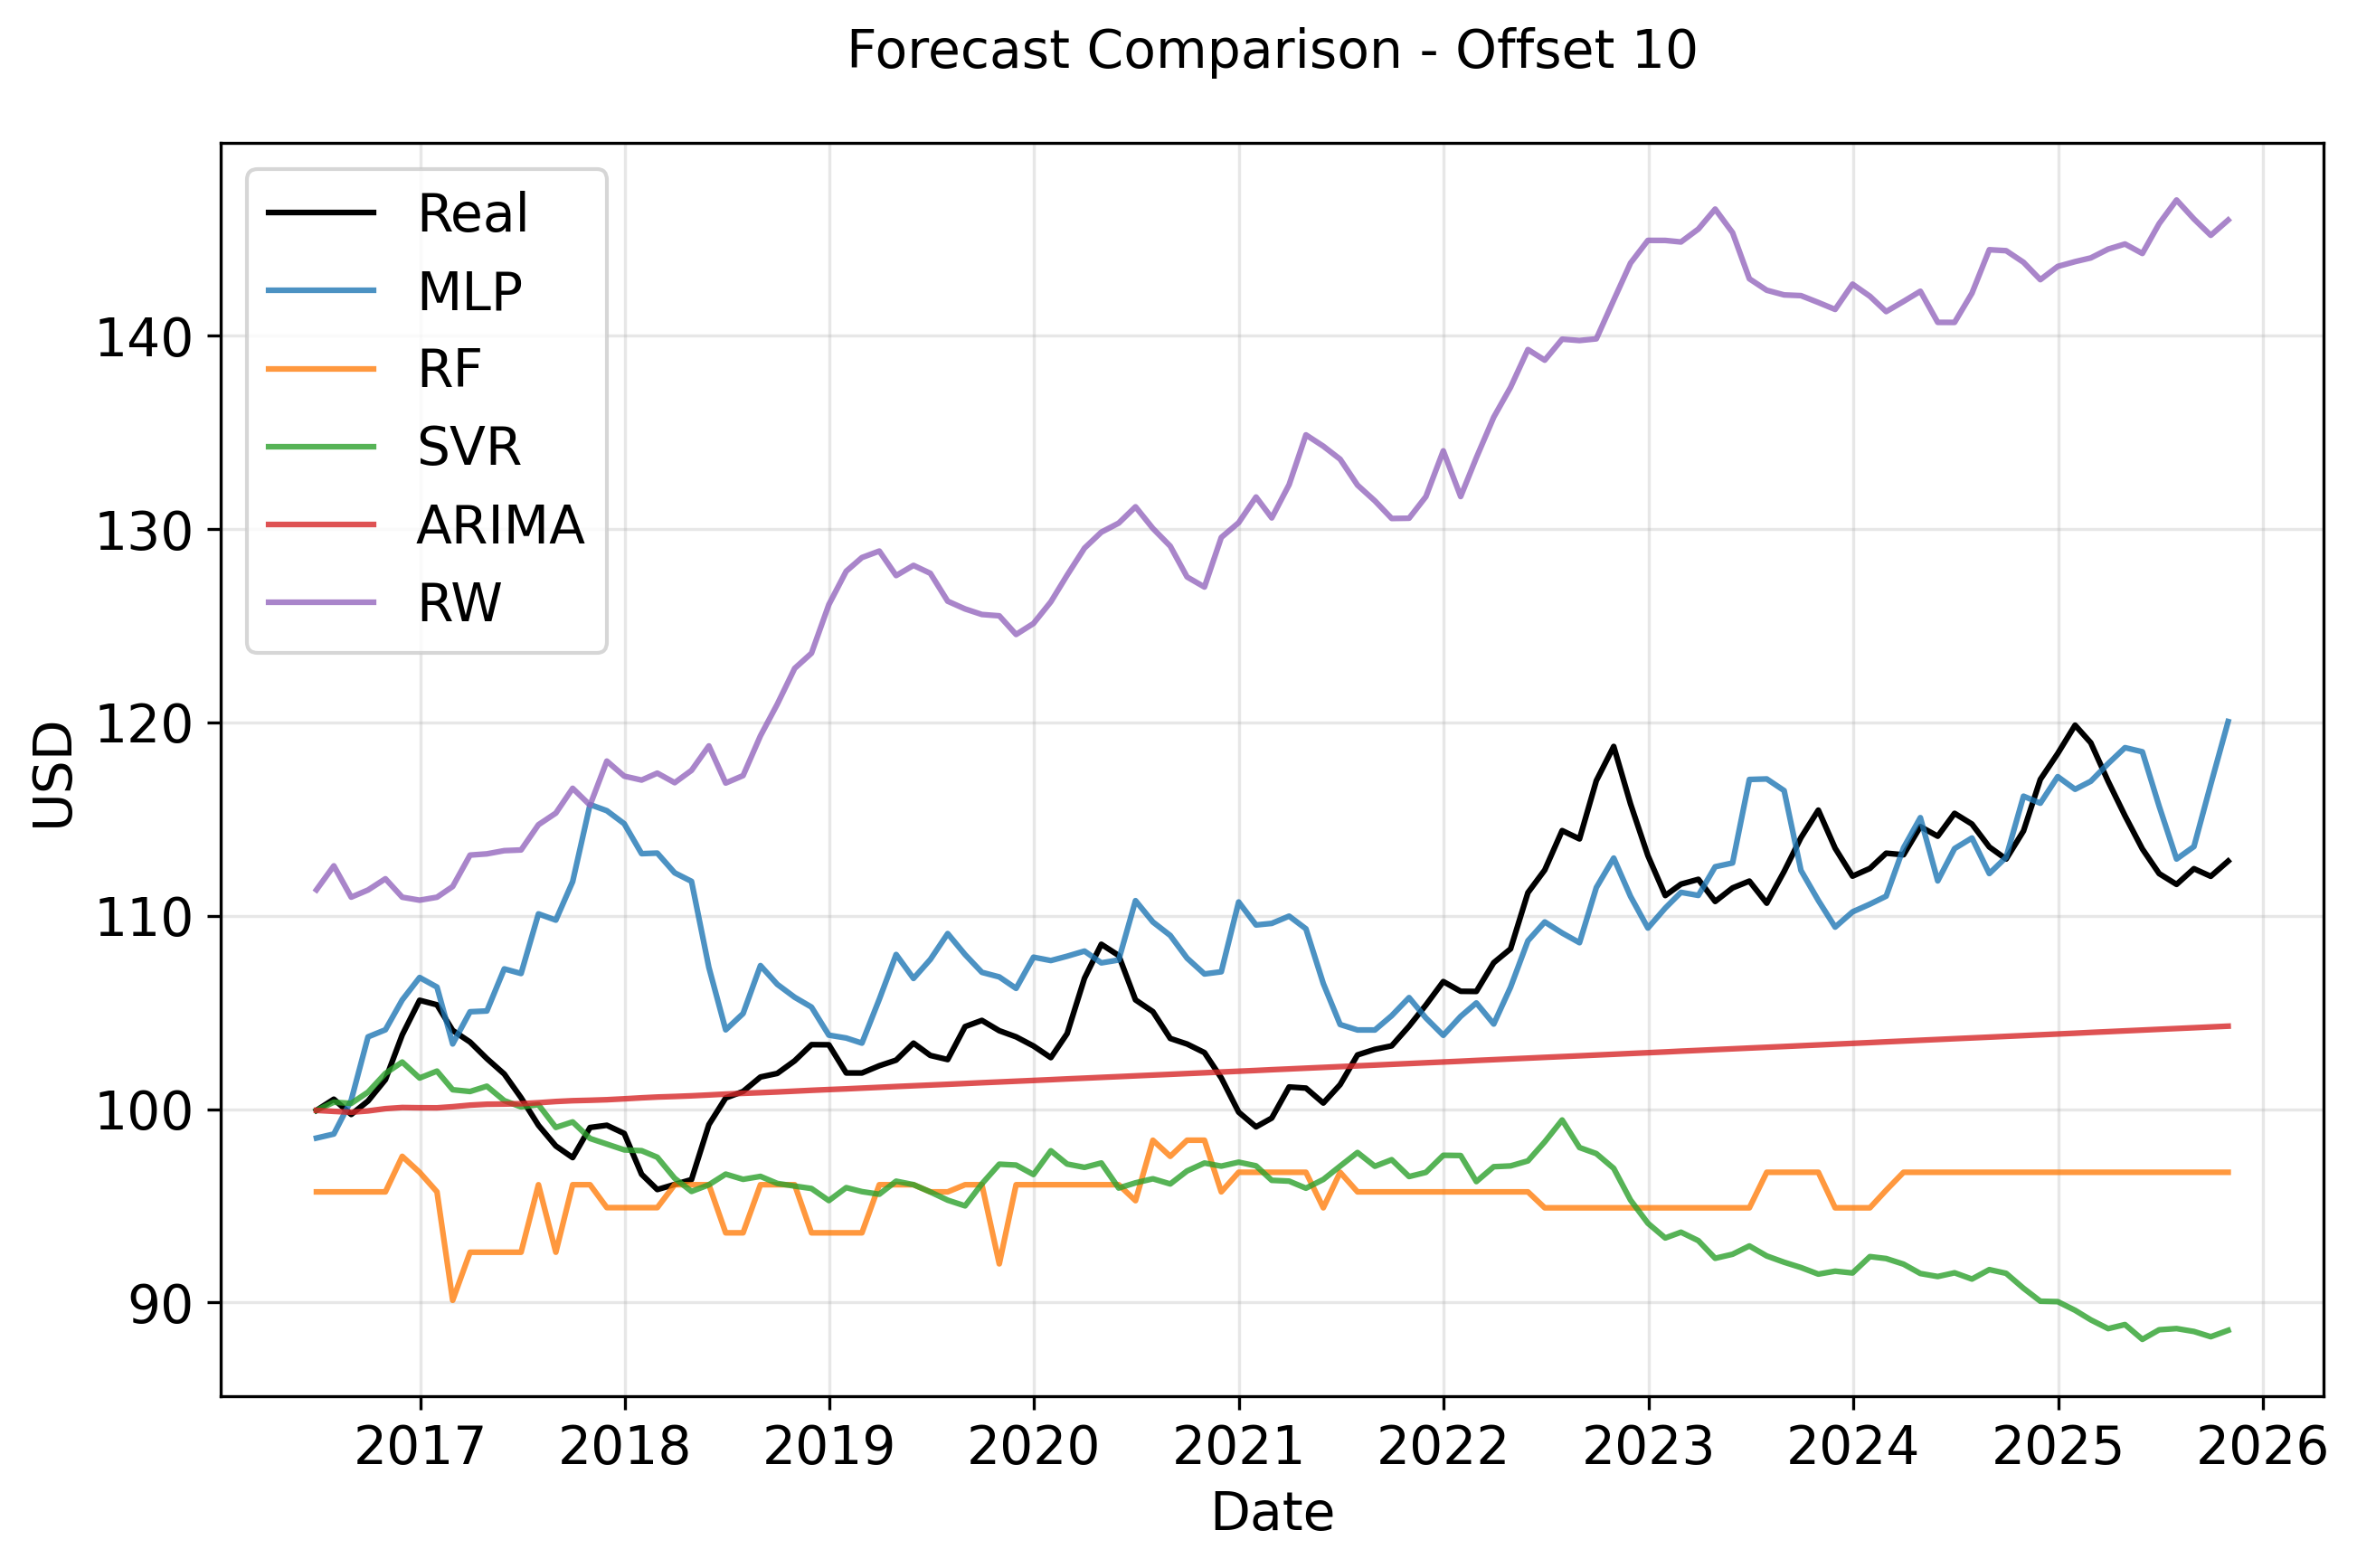
\includegraphics[width=\textwidth]{images/forecast-comparison/mse/10.png}
    \centering
    \caption{The best \gls{mse} forecasts per selected dataset per model for an offset of 10 months.}
    \label{fig:forecast-cmp-10}
\end{figure}

\begin{figure}[h]
    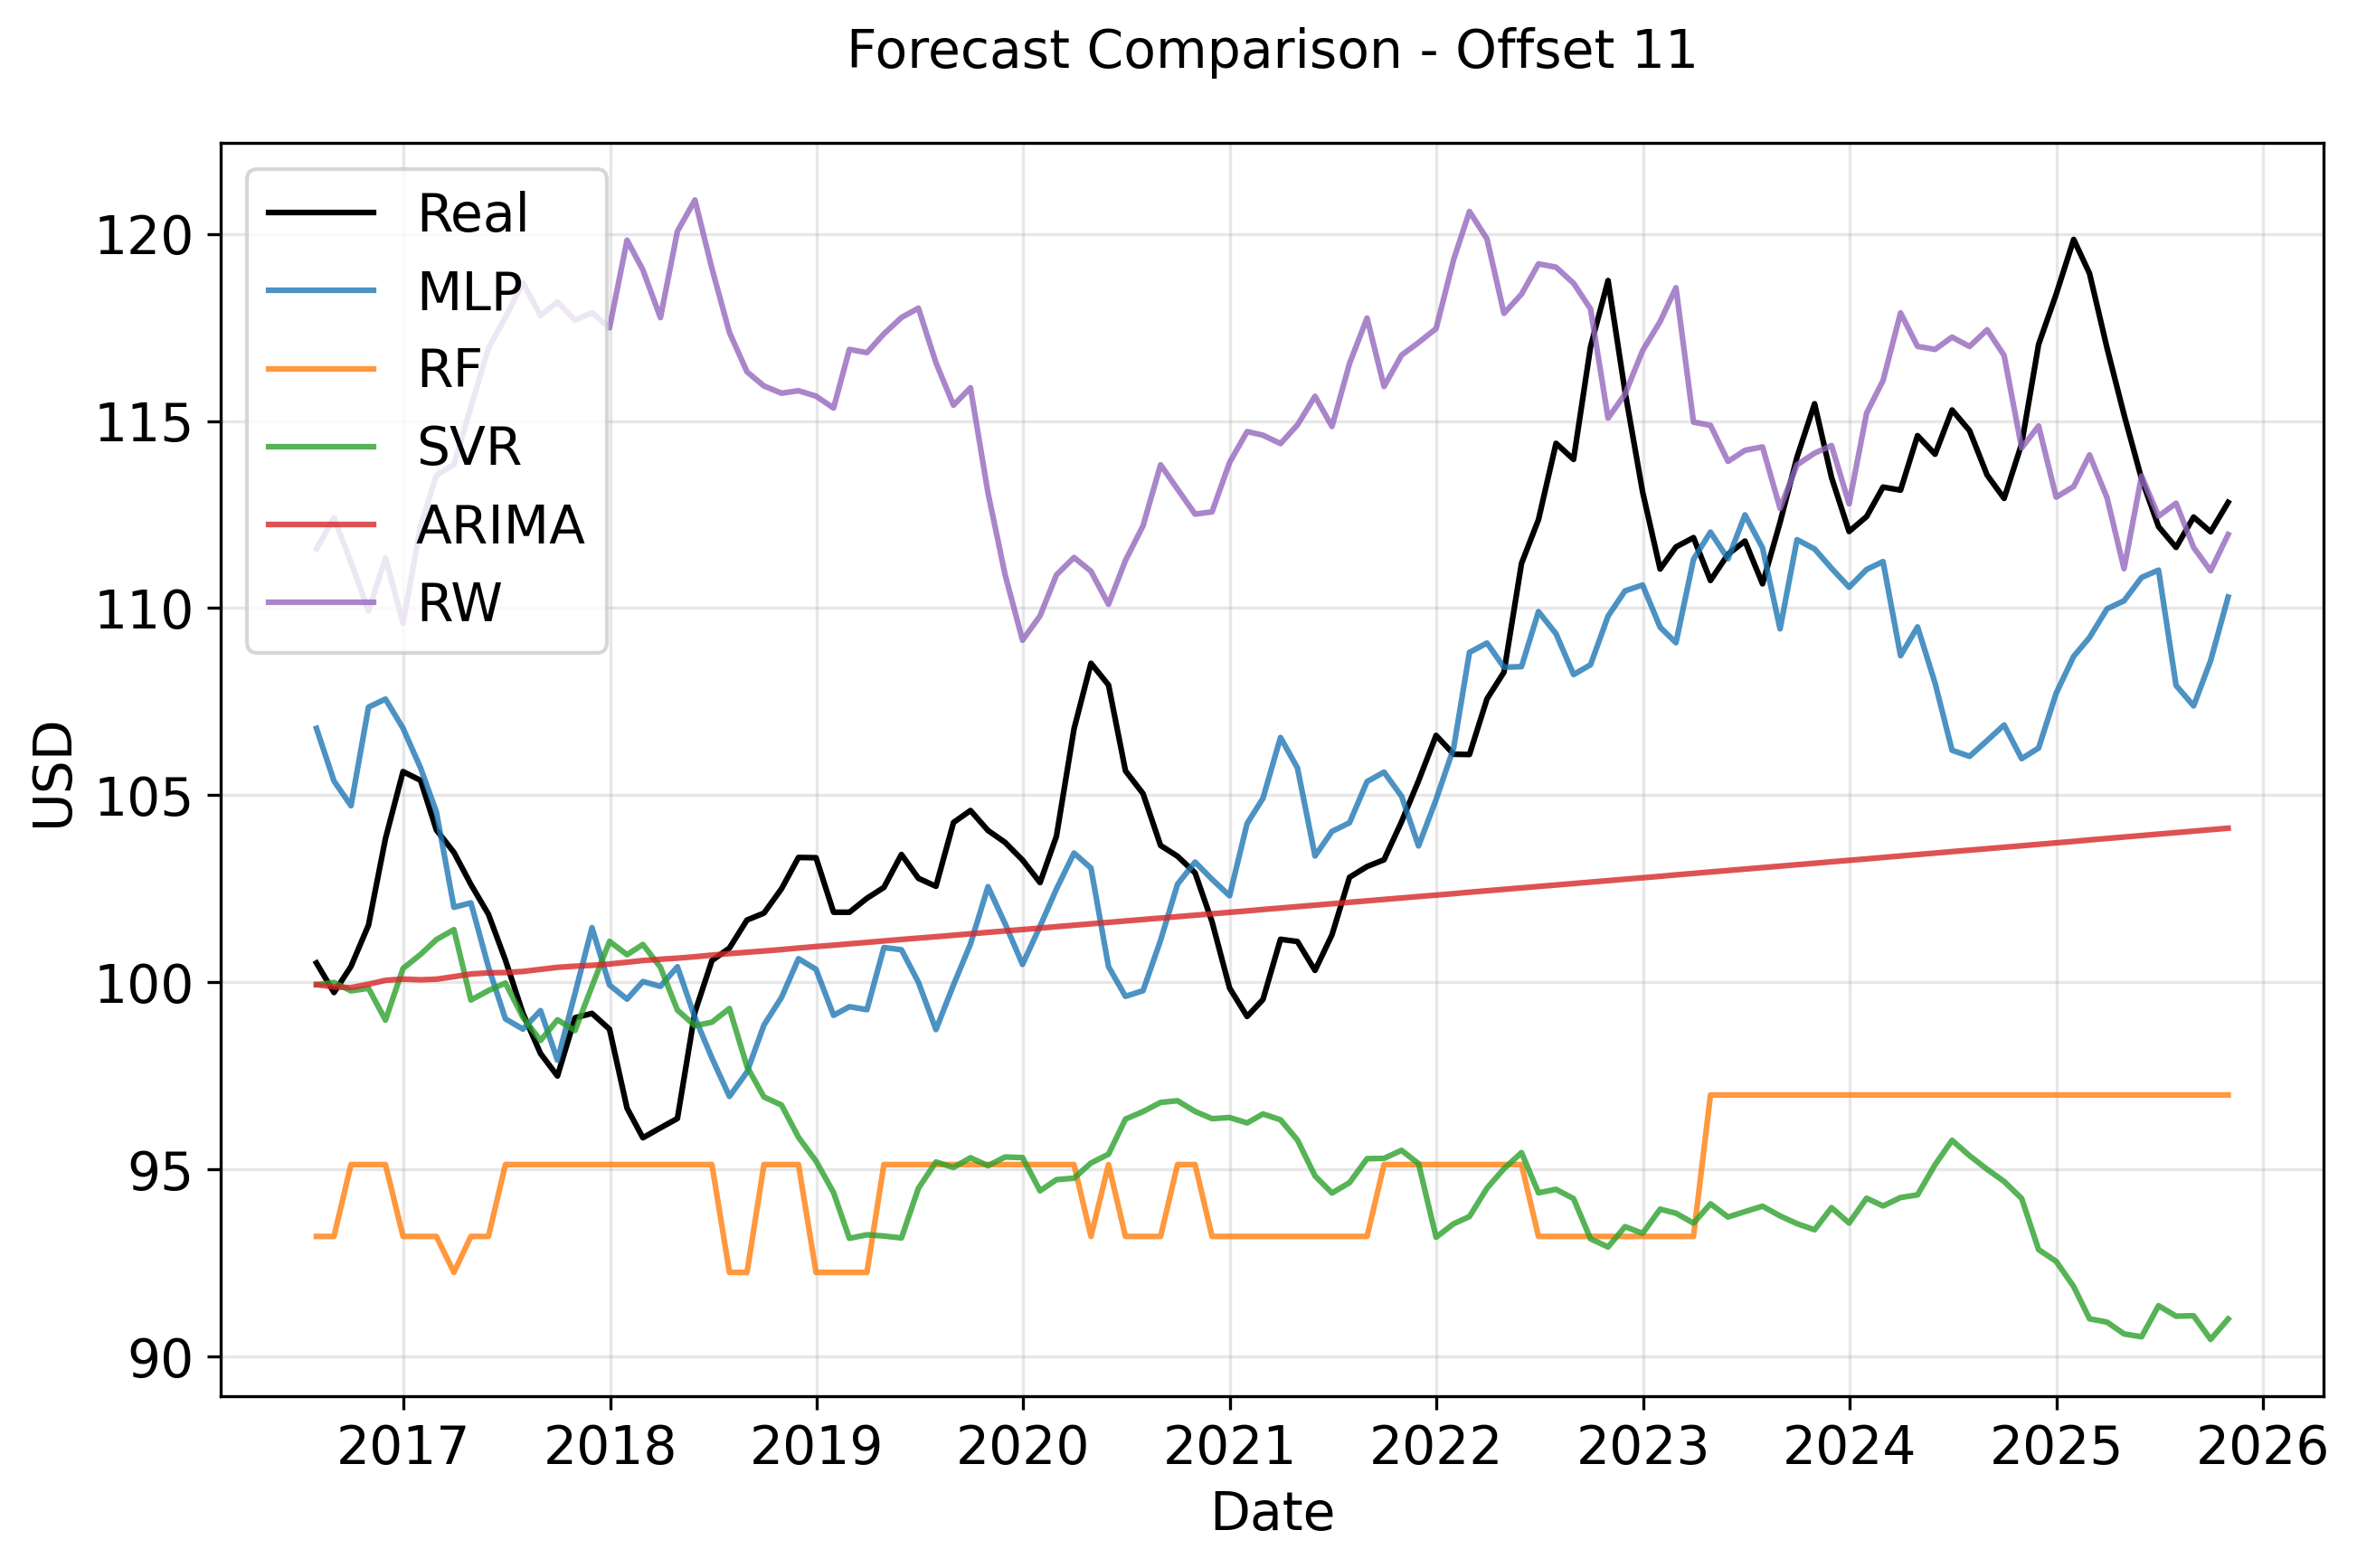
\includegraphics[width=\textwidth]{images/forecast-comparison/mse/11.png}
    \centering
    \caption{The best \gls{mse} forecasts per selected dataset per model for an offset of 11 months.}
    \label{fig:forecast-cmp-11}
\end{figure}

\begin{figure}[h]
    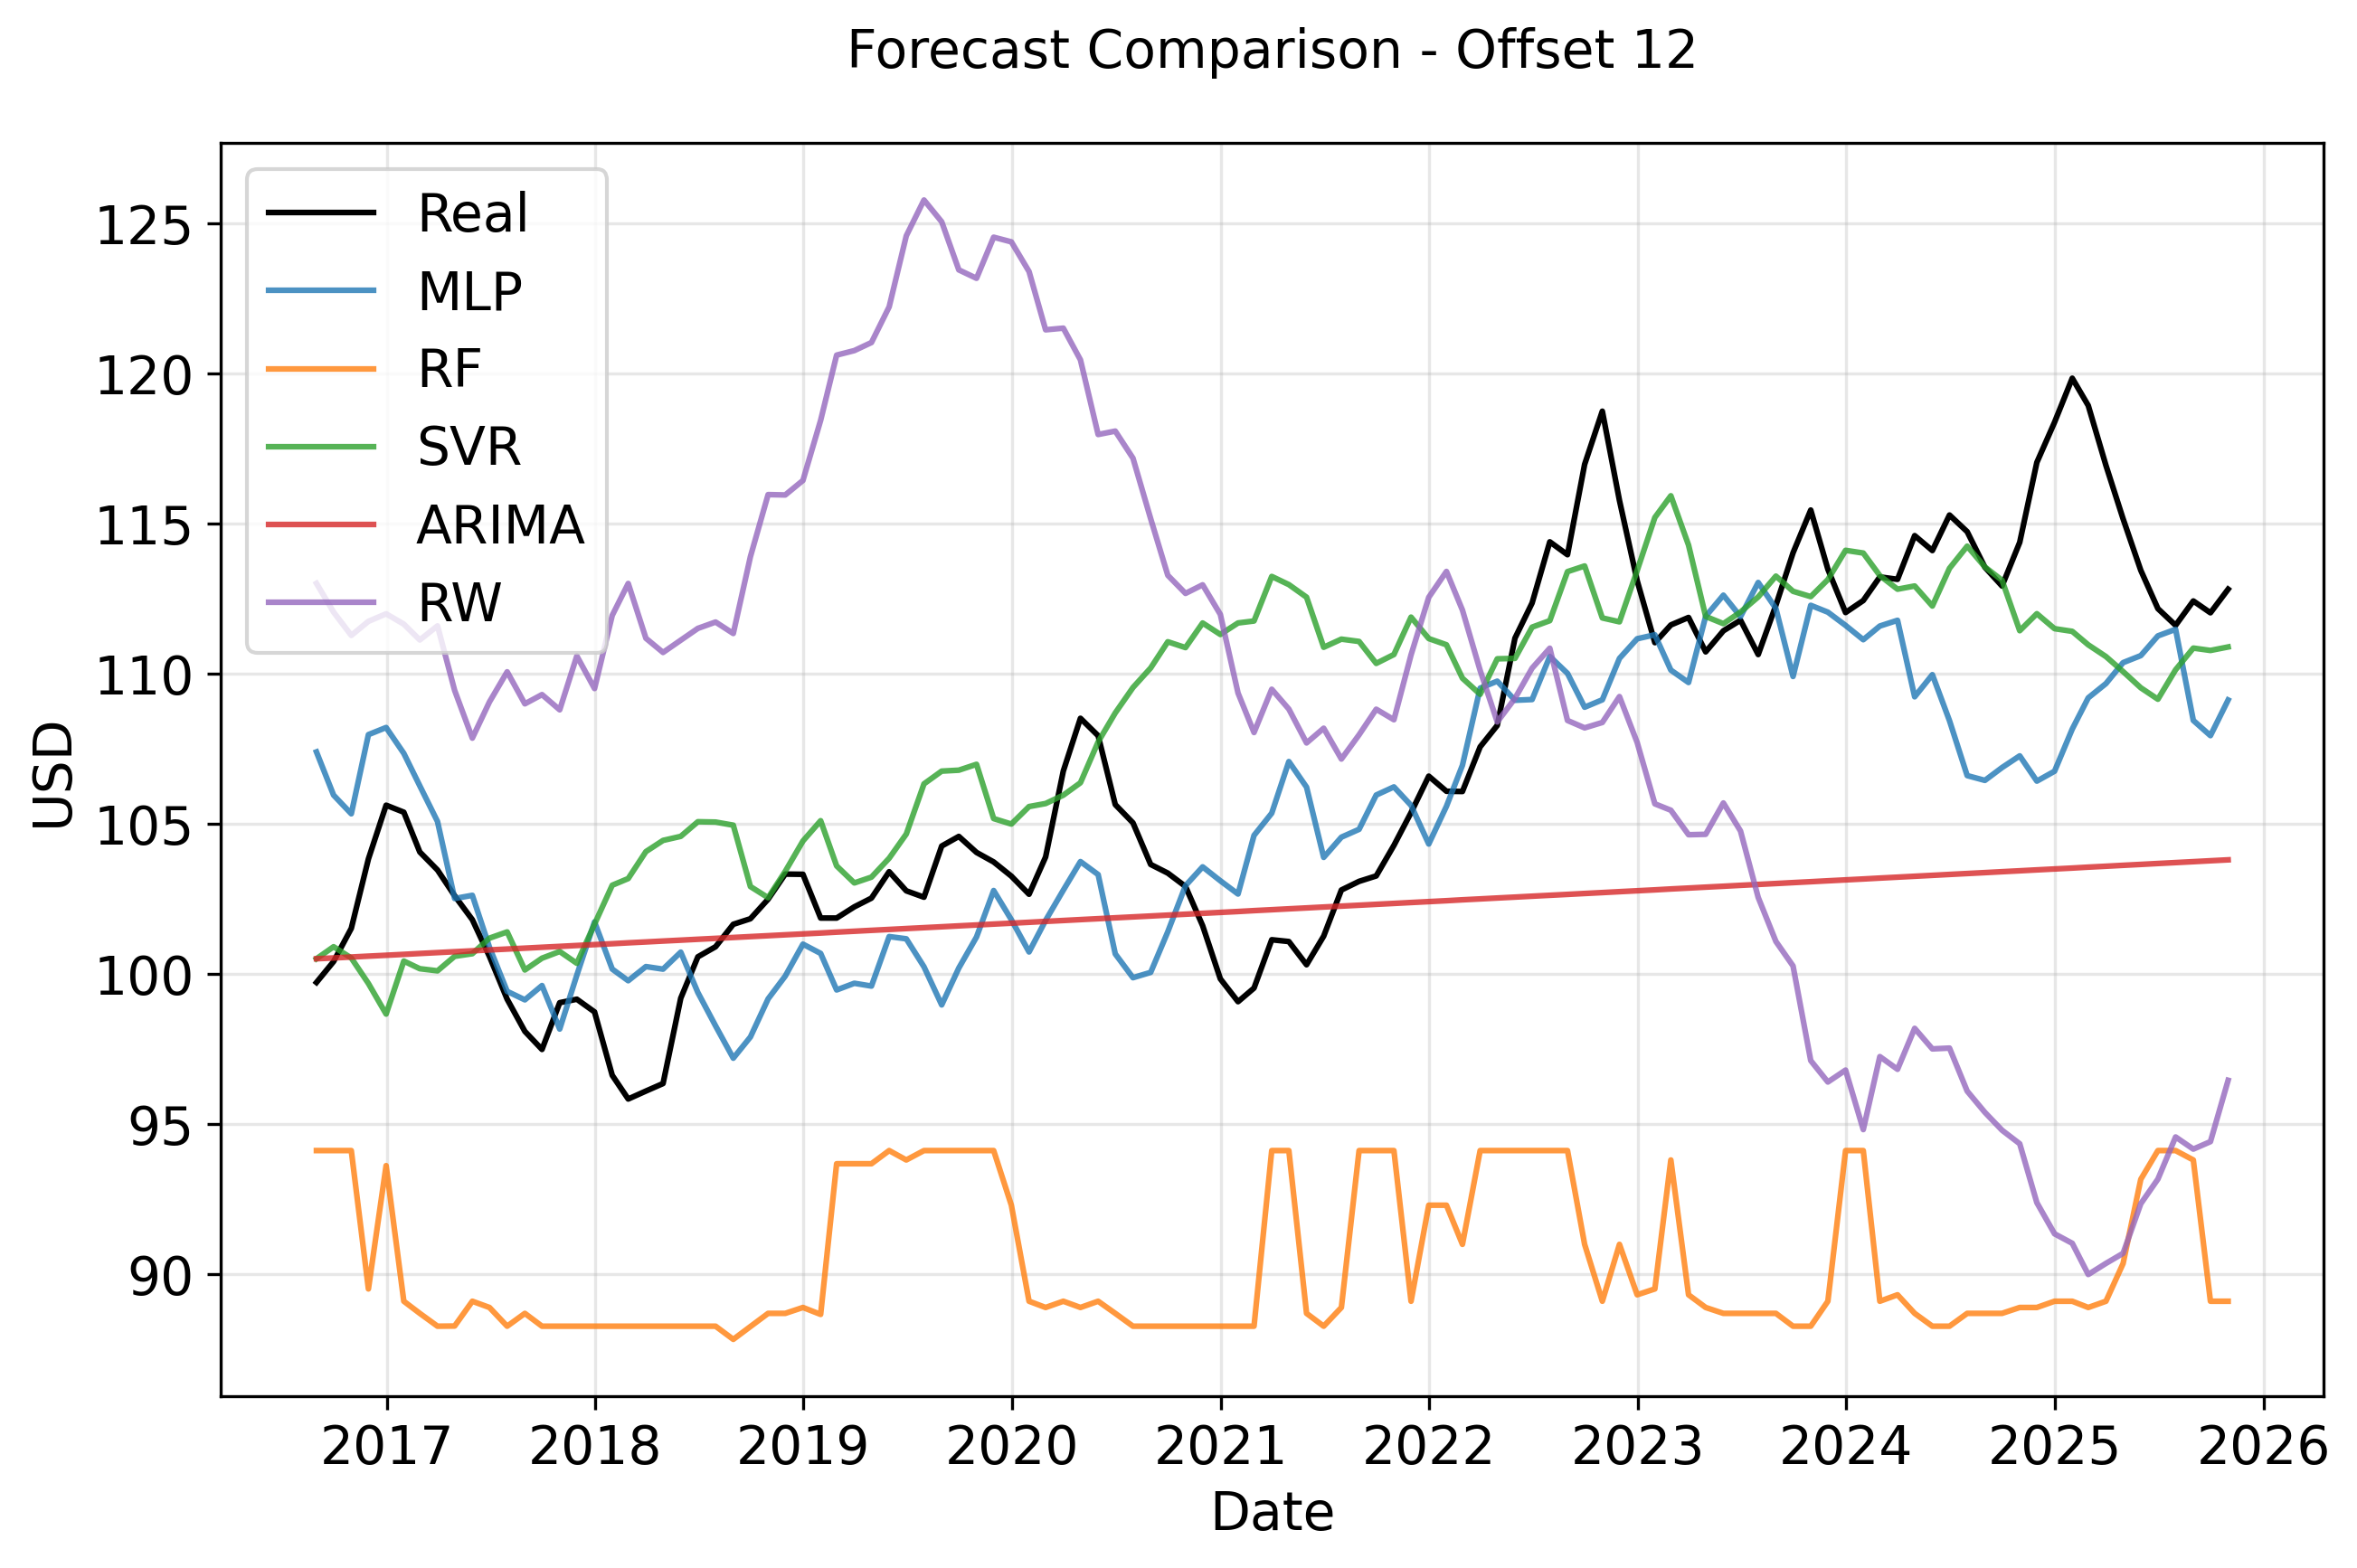
\includegraphics[width=\textwidth]{images/forecast-comparison/mse/12.png}
    \centering
    \caption{The best \gls{mse} forecasts per selected dataset per model for an offset of 12 months.}
    \label{fig:forecast-cmp-12}
\end{figure}


\section{Conclusions}\label{Conclusions}

In this paper an effort was made to fit three commonly used machine learning algorithms the \gls{mlp}, \gls{rf} and \gls{svr} models on multivariate currency exchange rate data. This was done in order to assess there applicability for forecasting.

Before the selected data could be used with the chosen models appropriate data preparation techniques had to be applied. As a first variables with missing values had to be removed. Next various combinations of intermediary preprocessing steps including log transformation, differencing and scaling were used to create multiple dataset variations for testing. After that came feature creation consisting of the duplication and application of a offset to each predictor variable. Multiple dataset were created with the offset applied ranging from 1 to 12 months. Following this step was feature selection allowing for the elimination of irrelevant feature variables and decorrelation allowing for the removal of all but one of every set of remaining intercorrelated feature variables. The final step of data preparation was the splitting of the dataset into train and test subsets in a 70:30 proportion. Once these steps were completed the models could be applied to the data. Since each model but the \gls{rf} has specific requirements for optimal model performance not all dataset variations were applied to all models.

All models were fitted on the prepared data using the Optuna hyperparameter optimization framework with the exception of the \gls{rw} model that did not require any fitting. For each model the most suitable data preprocessing variation was selected on the basis of the cumulative average \gls{mse}. Once selected the best values of each result for both metrics between models were compared. On the basis of figure \ref{fig:mse-model-cmp} for the \gls{mse} the best performing models are the \gls{mlp} followed by \gls{svr}, \gls{rf}, \gls{arima} and finally \gls{rw}.

In figure \ref{fig:cumulative-mse} comparing the average \gls{mse} of each best model - dataset combination for each offset a common tendancy is visible and shared by all models. The greater the offset the greater the error. All machine learning models exceeded the performance of the \gls{rw} model with few exceptions. In regards to the \gls{arima} model the results are varied with only the \gls{mlp} exceeding its performance with one exception, while the \gls{rf} and \gls{svr} models exhibitng worse performance in over half of the offsets.



\clearpage

\printglossary

\clearpage

\emergencystretch=1em
\printbibliography[heading=bibintoc, title={References}]

\end{document}
